\documentclass[final]{cpecmu}

%% This is a sample document demonstrating how to use the CPECMU
%% project template. If you are having trouble, see "cpecmu.pdf" for
%% documentation.

\projectNo{P003-2}
\acadyear{2021}

\titleTH{ระบบแสดงความคืบหน้าในการสำเร็จการศึกษา}
\titleEN{Visualization system for graduation requirement fulfillment}

\author{นายชุติพนธ์ วิมลกาญจนา}{Chutipon Vimonkanjana}{610610578}
\author{นายอานนท์ รอดตัว}{Arnon Rottua}{610610625}

\cpeadvisor{chinawat}
\cpecommittee{pruet}
\cpecommittee{navadon}


%% Some possible packages to include:
\usepackage[final]{graphicx} % for including graphics

%% Add bookmarks and hyperlinks in the document.
\PassOptionsToPackage{hyphens}{url}
\usepackage[colorlinks=true,allcolors=Blue4,citecolor=red,linktoc=all]{hyperref}
\def\UrlLeft#1\UrlRight{$#1$}

%% Needed just by this example, but maybe not by most reports
\usepackage{afterpage} % for outputting
\usepackage{pdflscape} % for landscape figures and tables. 

%% Some other useful packages. Look these up to find out how to use
%% them.
% \usepackage{natbib}    % for author-year citation styles
% \usepackage{txfonts}
% \usepackage{appendix}  % for appendices on a per-chapter basis
% \usepackage{xtab}      % for tables that go over multiple pages
\usepackage{subfigure} % for subfigures within a figure
\usepackage{float}
% \usepackage{pstricks,pdftricks} % for access to special PostScript and PDF commands
% \usepackage{nomencl}   % if you have a list of abbreviations

%% if you're having problems with overfull boxes, you may need to increase
%% the tolerance to 9999
% \tolerance=9999

\bibliographystyle{plain}
% \bibliographystyle{IEEEbib}

% \renewcommand{\topfraction}{0.85}
% \renewcommand{\textfraction}{0.1}
% \renewcommand{\floatpagefraction}{0.75}

%% Example for glossary entry
%% Need to use glossary option
%% See glossaries package for complete documentation.
\ifglossary
  \newglossaryentry{lorem ipsum}{
    name=lorem ipsum,
    description={derived from Latin dolorem ipsum, translated as ``pain itself''}
  }
\fi

%% Uncomment this command to preview only specified LaTeX file(s)
%% imported with \include command below.
%% Any other file imported via \include but not specified here will not
%% be previewed.
%% Useful if your report is large, as you might not want to build
%% the entire file when editing a certain part of your report.
% \includeonly{final-chapters/intro,final-chapters/background}

\begin{document}
\maketitle
\makesignature

\ifproject
\begin{abstractTH}
    เป้าหมายหลักของการทําโปรเจคนี้เกิดจาก ในปัจจุบันมีหลักสูตรที่คิดขึ้นและถูกใช้ในมหาวิทยาลัยอย่าง หลากหลายโดยใน
    แต่ละหลักสูตรนั้นก็จะมีโครงสร้างที่แตกต่างกันออกไป ถึงแม้ว่าจะเป็นหลักสูตรที่ถูกใช้ในคณะ หรือสาขาเดียวกันแต่ถ้าเป็นคนละ
    หลักสูตร ก็จะมีโครงสร้างของหลักสูตรที่แตกต่างกันอย่างแน่นอนเพราะเกิดการปรับปรุงทั้งเนื้อหาเเละโครงสร้างของหลักสูตรเพื่อ
    ความทันสมัยขององค์ความรู้ ยกตัวอย่างเช่น หลักสูตรปี การศึกษา 2558 และ หลักสูตรปี การศึกษา 2563 ของคณะ
    วิศวกรรมศาสตร์ สาขาวิศวกรรมคอมพิวเตอร์ เมื่อนําเอาโครงสร้างของหลักสูตรมาเปรียบเทียบกันดูแล้ว จะพบว่ามีข้อแตกต่างกันใน
    บางส่วน และมีความเหมือนกันในบางส่วนเช่นกัน ซึ่งในแต่ละหลักสูตรก็จะมีความซับซ้อนของโครงสร้างหลักสูตรที่แตกต่างกันออกไป
    ตามเกณฑ์ที่แต่ละคณะกําหนด ซึ่งในปัจจุบันเว็บไซต์ของสํานักทะเบียนนั้นมีความล้าสมัยในส่วนที่จะแสดงโครงสร้างของแต่ละ
    หลักสูตร รวมไปถึงบางฟังก์ชันที่เกิดข้อผิดพลาด (bug) และยังใช้เวลานานในการประมวลผล เช่น การแสดงข้อมูล หลักสูตร
    รายบุคคลของนักศึกษาที่ยังไม่มีความละเอียดมากพอ และในการแก้ไขหลักสูตรในแต่ละครั้งของอาจารย์ ผู้สอนนั้นมีความยากลําบาก
    เช่น การเพิ่มวิชาเลือกเข้าไปในหลักสูตรทุกหลักสูตรของสาขาวิศวกรรมคอมพิวเตอร์ จําเป็นที่จะต้องเพิ่มทีละวิชาในทุกหลักสูตรที่
    ภาควิชามีทําให้เสียเวลานานพอสมควร ดังนั้นโครงงานนี้จึงมุ่งที่จะ แก้ไขปัญหาและอุปสรรคดังกล่าว โดยการสร้างโปรแกรมประยุกต์
    บนเว็บ (web application) สําหรับจัดการข้อมูลและโครงสร้างในแต่ละหลักสูตรให้มีความเข้าใจง่ายและสะดวกต่อการแก้ไข เพื่อ
    เพิ่มประสิทธิภาพในการใช้ งาน โดยมีความสามารถที่จะรองรับหลักสูตรในมหาวิทยาลัย รวมไปถึงเพิ่มส่วนที่จะช่วยเเสดงข้อมูล
    การศึกษาของ นักศึกษาอย่างละเอียดให้กับอาจารย์ที่ปรึกษาและตัวนักศึกษาเอง อาทิเช่น การแสดงรายวิชาที่ยังไม่ได้ทําการ
    ลงทะเบียน และการคํานวณเกรดล่วงหน้า เป็นต้น
\end{abstractTH}

\begin{abstract}
    The main goal of doing this project comes from At present, 
    there are courses that are invented and used in universities like There are many different courses 
    in which each course is structured differently. Although it is a course that is used in the Faculty or 
    the same branch, but if it is a different course There will definitely be a different course structure 
    because both the content and the course structure are updated for the modernization of the body of knowledge. 
    For example, the 2015 academic year program and the 2020 academic year program of the Faculty of Engineering. 
    Computer Engineering When comparing the structure of the curriculum You will find that there are some differences. 
    And they are the same in some parts as well. Each course has a different complexity of course structure according to 
    the criteria set by each faculty. Currently, the registrar's website is outdated in terms of showing the structure of 
    each course, including some functions that have bugs (bugs) and take a long time to process, such as displaying information.
     Individual courses of students that are not yet detailed enough and in the course of each revision of the teacher Instructors 
     have difficulties such as adding elective courses to all courses in computer engineering. It is necessary to add one 
     subject at a time to every course the department has, which takes a considerable amount of time. Therefore, 
     this project aims to solve such problems and obstacles By creating a web application (web application) to manage 
     the data and structure in each course to be easy to understand and easy to edit. To increase the efficiency of 
     use with the ability to support the courses in the university including adding a section that will help display 
     the educational information of students in detail to the advisors and students themselves, such as showing courses 
     that have not yet been registered and calculating grades in advance, etc.
\end{abstract}

\iffalse
\begin{dedication}
Dedication page is optional.
\end{dedication}
\fi % \iffalse

\begin{acknowledgments}
    โครงงานนี้ได้รับความกรุณาจาก อ.ดร.ชินวัตร อิศราดิสัยกุล อาจารย์ที่ปรึกษาที่ได้สละเวลาให้ความช่วยเหลือ ให้คำแนะนำ ให้ความรู้และแนวคิดต่างๆ รวมไปถึงขอขอบคุณอาจารย์คณะกรรมการทั้ง 
    อ.ดร.พฤษภ์ บุญมา และ ผศ.ดร.นวดนย์ คุณเลิศกิจ ที่ให้คำแนะนำต่างๆ รวมไปถึงเพื่อนๆที่ให้กำลังใจและคำแนะนำที่ดีตลอดการทำโครงงานที่ผ่านมา จนทำโครงงานเล่มนี้ออกมาได้อย่างเสร็จสมบูรณ์
    นอกจากนี้ผู้จัดทําขอขอบพระคุณบิดา-มารดาที่ได้ให้ชีวิต เลี้ยงดูสั่งสอน และส่งเสียให้ผู้จัดทําได้ศึกษาเล่าเรียนจนจบหลักสูตรปริญญาตรี หลักสูตรวิศวกรรมศาสตร์บัณฑิต ซึ่งท่านได้ให้กําลังใจในวันที่ยากลําบากและยังเป็นแรงผลักดันให้สร้างสรรค์ผลงานและมุ่งมั่นจนทําให้โครงงานนี้สําเร็จ รวมทั้งขอขอบพระคุณอีกหลายๆท่านที่ไม่ได้เอ่ยนามมา ณ ที่นี้ ที่ได้ให้ความช่วยเหลือตลอดมา หากหนังสือโครงงานเล่มนี้ผิดพลาดประการใด ทางผู้จัดทําขอยอมรับด้วยความยินดี

\acksign{2022}{10}{10}
\end{acknowledgments}%
\fi % \ifproject

\contentspage

\ifproject
\figurelistpage

\tablelistpage
\fi % \ifproject

% \abbrlist % this page is optional

% \symlist % this page is optional

% \preface % this section is optional


\pagestyle{empty}\cleardoublepage
\normalspacing \setcounter{page}{1} \pagenumbering{arabic} \pagestyle{cpecmu}

\chapter{\ifenglish Introduction\else บทนำ\fi}

\section{\ifenglish Project rationale\else ที่มาของโครงงาน\fi}
การที่จะสําเร็จการศึกษาได้นั้น นักศึกษาจําเป็นที่จะต้องเรียนวิชาให้ครบเกณฑ์ของแต่ละภาควิชาตามที่สถานศึกษากําหนด
ซึ่งสามารถลงเรียนตามแผนการเรียนรายเทอมตามที่ภาควิชาออกแบบมาให้ได้ แต่การที่นักศึกษาจะลงทะเบียนเรียนในแต่ละเทอมให้
เป็นไปตามแผนการเรียนดังกล่าวนั้นเป็นไปด้วยความยากลําบาก เนื่องจากว่ามีปัจจัยหลายด้านที่ทําให้นักศึกษาไม่สามารถเรียนวิชา
ตามแผนที่กําหนดหรือไม่สามารถสําเร็จกระบวนวิชาได้ในเทอมนั้น เช่น ได้รับอักษร F หรือ W ส่งผลให้วิชาที่เป็นวิชาต่อต้องลงเรียน
ถัดไปในอีกหนึ่งเทอมหรือมากกว่า ซึ่งจะทําให้นักศึกษาเกิดความสับสนในการวางแผนการเรียนของตนเองและไม่มั่นใจว่าตนเอง
สําเร็จกระบวนวิชาในแต่ละหมวดครบแล้วหรือยัง และอาจเกิดปัญหาการลงเรียนวิชาในหมวดนั้นจนเกินความจําเป็น ทําให้เสียเวลา
และหน่วยกิตในเทอมนั้นโดยใช่เหตุ ซึ่งหากจะทําการตรวจสอบด้วยตัวเองโดยการไล่ดูในหมวดนั้นๆว่าลงเรียนวิชาตามเกณฑ์ในหมวด
ครบแล้วหรือยัง จึงเป็นเรื่องที่ยุ่งยาก และเสียเวลาเพราะจําเป็นต้องทําแบบดั่งกล่าวในทุกเทอม
ดังนั้นพวกเราจึงได้คิดหาวิธีแก้ปัญหาโดยการทํา web application ที่ช่วยตรวจสอบกระบวนวิชาในแต่ละหมวดว่า
นักศึกษาสําเร็จวิชาตามเกณฑ์ที่กําหนดในแต่ละหมวดแล้วหรือไม่ เพื่อลดปัญหาการลงเรียนวิชาในหมวดจนเกินความจําเป็น และ
ประหยัดเวลาในการตรวจสอบวิชาที่ตัดสินใจจะลงทะเบียนเรียนของนักศึกษาในแต่ละเทอม นอกจากนี้นักศึกษาสามารถตรวจสอบ
ความคืบหน้าในการสําเร็จการศึกษาตามความถนัดพิเศษ และชนิดของแผนการเรียนที่ตนเองสนใจได้

\section{\ifenglish Objectives\else วัตถุประสงค์ของโครงงาน\fi}
\begin{enumerate}
    \item เพื่อพัฒนา web application ระบบแสดงความคืบหน้าในการสำเร็จการศึกษา สําหรับนักศึกษา อาจารย์ที่ปรึกษา 
    และผู้ดูแลหลักสูตรของมหาวิทยาลัยเชียงใหม่ โดยมีความสามารถดังนี้
\begin{itemize}
    \item ช่วยเเสดงความคืบหน้าในการศึกษาของนักศึกษาได้อย่างถูกต้อง เพื่อเป็นตัวช่วยในการตรวจสอบ เเละลงทะเบียนรายวิชาให้ครบตามกําหนดของหลักสูตร
    \item ช่วยเเบ่งเบาภาระของอาจารย์ที่ปรึกษา ในการตรวจสอบสถานะการสําเร็จการศึกษาของนักศึกษา
    \item ช่วยให้ ผู้พัฒนาระบบสามารถจัดการกับหลักสูตรได้อย่างมีประสิทธิภาพ รองรับหลักสูตรที่มีอยู่ในปัจจุบัน เเละอนาคต
\end{itemize}  
\end{enumerate}

\section{\ifenglish Project scope\else ขอบเขตของโครงงาน\fi}

\subsection{\ifenglish Hardware scope\else ขอบเขตด้านข้อมูล\fi}
\begin{enumerate}
    \item หลักสูตรการศึกษาในระดับปริญญาตรีทุกหลักสูตรของมหาวิทยาลัยเชียงใหม่ ยกเว้นระดับยากมาก ตั้งแต่ปี พ.ศ.2558 เป็นต้นมา
    \item ข้อมูลพื้นฐานทั่วไปของนักศึกษา(OAuth) ข้อมูลพื้นฐานเพิ่มเติมของนักศึกษา(Database ของมหาวิทยาลัย) ข้อมูลการลงทะเบียนรายวิชาของนักศึกษา(Database ของมหาวิทยาลัย)
\end{enumerate}

\subsection{\ifenglish Software scope\else ขอบเขตด้านซอฟต์แวร์\fi}
\begin{itemize}
    \item นักศึกษา
    \begin{enumerate}
        \item ระบบทําหน้าที่หลักในการรายงานความคืบหน้าของการศึกษา จนถึงตรวงสอบการสําเร็จการศึกษา 
        ไม่สามารถถูกใช้ในการวางเเผนการเรียนเเบบรายเทอม ดูตัวต่อวิชา หรือคํานวณเวลาที่จะจบการศึกษาในอนาคตได้
    \end{enumerate}
    \item อาจารย์ที่ปรึกษา
    \begin{enumerate}
        \item อาจารย์ที่ปรึกษาสามารถตรวจสอบได้ว่านักศึกษาที่ตนดูแลอยู่นั้นสําเร็จการศึกษาแล้ว ก็ต่อเมื่อนักศึกษาเข้ามาใช้งานระบบในส่วนของ นักศึกษาก่อนเเล้ว
    \end{enumerate}
    \item ผู้ดูเเลโครงสร้างหลักสูตร
    \begin{enumerate}
        \item ระบบไม่สามารถรองรับในหลักสูตรระดับยากมาก เพียงเเต่เเนวคิดในการออกเเบบระบบ สามารถนําไปใช้ประโยชน์เพิ่มเติมในหลักสูตรระดับยากได้
    \end{enumerate}
\end{itemize}


\section{\ifenglish Expected outcomes\else ประโยชน์ที่ได้รับ\fi}
\begin{itemize}
    \item นักศึกษา
    \begin{enumerate}
        \item สร้างความสะดวกในการตรวจสอบการสําเร็จการศึกษาของตนเอง
        \item ช่วยลดความสับสนในการทําความเข้าใจหลักสูตรการศึกษาที่ตนศึกษาอยู่เพื่อเลือกลงวิชาให้ครบในหมวดที่กําหนด
        \item สามารถเลือกวางแผนการศึกษาในหลักสูตรการศึกษาตามแบบที่ตนเองสนใจได้
        \item สร้างความมั่นใจได้ว่ากระบวนวิชาที่ตนศึกษาอยู่นั้นเป็นไปตามแผนการศึกษาของหลักสูตรหรือไม่
    \end{enumerate}
    \item อาจารย์ที่ปรึกษา
    \begin{enumerate}
        \item สร้างความสะดวกในการตรวจสอบความคืบหน้าการสําเร็จการศึกษาของนักศึกษาทั้งแบบรายบุคคล และแบบ
        กลุ่ม
        
    \end{enumerate}
    \item ผู้ดูเเลโครงสร้างหลักสูตร
    \begin{enumerate}
        \item ช่วยลดเวลาในการจัดการหลักสูตร เนื่องจากเเนวคิดการออกเเบบ Data model 
        ที่จะรวมข้อมูลที่มีการ share เข้าด้วยกัน ทําให้สามารถจัดการข้อมูลเเค่เพียงที่้เดียว เเต่ส่งผลไปหลายหลักสูตร
    \end{enumerate}
\end{itemize}

\section{\ifenglish Technology and tools\else เทคโนโลยีและเครื่องมือที่ใช้\fi}

% \subsection{\ifenglish Hardware technology\else เทคโนโลยีด้านฮาร์ดแวร์\fi}

\subsection{\ifenglish Software technology\else เทคโนโลยีด้านซอฟต์แวร์\fi}
\begin{enumerate}
\item React ใช้เป็นเครื่องมือพัฒนาในส่วนของ frontend เพื่อพัฒนาหน้าเว็บแอพลิเคชันสําหรับแสดงผลข้อมูลต่างๆในส่วนติดต่อกับ ผู้ใช้งาน
\item NodeJS ใช้เป็น backend เพื่อประมวลผล เเละคํานวณข้อมูลเป็นหลัก เป็นศูนย์กลางในการติอต่อ database 
เชื่อมต่อ API ทั้ง REST API เเละ GraphQL API เเละเป็นที่รองรับการติดตั้ง packages เสริมเพิ่มเติมที่ระบบต้องการ
\item ExpressJS ใช้สร้าง server หลักของระบบที่จะตอบรับ request, response ที่เข้ามาจาก client(frontend) 
authentication(OAuth\cite{o}) เเละยังทํางานร่วมกับ REST API\cite{rest} เเละ GraphQL \cite{graphql}
\item REST API ถูกใช้เป็นหลักในการ ติดต่อกับ CMU-OAuth Server เพื่อทําการยืนยันตัวตนเข้าใช้งาน application 
เเละดึงข้อมูลนักศึกษาเบื้องต้นเพื่อมาประมวลผล
\item GraphQL ใช้เป็น API หลักในจัดการข้อมูลของหลักสูตร
\item MongoDB\cite{mongo} ใช้เป็นฐานข้อมูลหลักของระบบ
\end{enumerate}

\section{\ifenglish Project plan\else แผนการดำเนินงาน\fi}

\begin{plan}{6}{2021}{2}{2022}
    \planitem{6}{2021}{6}{2021}{ศึกษาปัญหาจากนักศึกษาและอาจารย์ที่ปรึกษา}
    \planitem{6}{2021}{8}{2021}{ศึกษาโครงสร้างหลักสูตรแต่ละหลักสูตร}
    \planitem{7}{2021}{8}{2021}{ศีกษาเทคโนโลยที่ใช้}
    \planitem{9}{2021}{10}{2021}{เขียนโครงร่างรายงาน}
    \planitem{7}{2021}{9}{2021}{ออกแบบระบบโดยรวม และขั้นตอนการใช้งานระบบ}
    \planitem{9}{2021}{11}{2021}{ออกแบบ UX/UI}
    \planitem{9}{2021}{11}{2021}{ออกแบบ database และ data model}
    \planitem{11}{2021}{2}{2022}{พัฒนาส่วนของ front-end ครั้งที่ 1 (แสดงรายวิชาในหน้านักศึกษา)}
    \planitem{11}{2021}{2}{2022}{พัฒนาส่วนของ back-end ครั้งที่ 1 (สร้าง data model)}
    \planitem{12}{2021}{3}{2022}{พัฒนาส่วนของ front-end ครั้งที่ 2 (แสดงแผนผังต้นไม้สำหรับหนัานักศึกษา)}
    \planitem{12}{2021}{2}{2022}{เรียนรู้การใช้งาน MongoDB และ Mongoose}
\end{plan}
\begin{plan}{3}{2022}{11}{2022}
    \planitem{3}{2022}{5}{2022}{พัฒนาส่วนของ front-end ครั้งที่ 3 (หน้าผู้ดูแลหลักสูตร)}
    \planitem{3}{2022}{5}{2022}{ศึกษา Graphql และ TypeScript สำหรับเขียน back-end}
    \planitem{5}{2022}{5}{2022}{พัฒนาส่วนของ front-end ครั้งที่ 4 (แบบฟอร์มสำหรับเพิ่มคณะและสาขาวิชา)}
    \planitem{6}{2022}{7}{2022}{พัฒนา front-end ครั้งที่ 5 (แบบฟอร์มเลือกแผนการเรียนในหน้านักศึกษา)}
    \planitem{6}{2022}{7}{2022}{พัฒนา back-end (การใช้ filter ในการเลือก path )}
    \planitem{6}{2022}{7}{2022}{เชื่อม front-end เข้ากับ back-end เพื่อทดสอบ flow ของระบบ}
    \planitem{8}{2022}{8}{2022}{เชื่อมต่อข้อมูลกับมหาวิทยาลัยผ่านระบบ OAuth}
    \planitem{8}{2022}{9}{2022}{พัฒนา front-end ครั้งที่ 6 (หน้าสำหรับ login ผ่าน OAuth และหน้าอาจารย์ที่ปรึกษา)}
    \planitem{10}{2022}{10}{2022}{พัฒนา front-end ครั้งที่ 7 (เพิ่มเติมส่วนต่างๆ จากคำแนะนำของอาจารย์ที่ปรึกษาและคณะกรรมการ)}
    \planitem{10}{2022}{10}{2022}{พัฒนา back-end (การตรวจสอบข้อมูลและการสำเร็จการศึกษาของนักศึกษา)}
    \planitem{9}{2022}{11}{2022}{เขียน final report }
    \planitem{11}{2022}{11}{2022}{เก็บ feedback เพิ่มเติมจากการทดลองใช้เว็บแอบพลิเคชัน}
\end{plan}

\section{\ifenglish Roles and responsibilities\else บทบาทและความรับผิดชอบ\fi}
การพัฒนาระบบถูกเเบ่งออกเป็น 2 ส่วน 
\begin{enumerate}
    \item นายชุติพนธ์ วิมลกาญจนา รับหน้าที่ Backend developer รับผิดชอบเรื่อง Database design, API design, Data manipulation
    \item นายอานนท์ รอดตัว รับหน้าที่ Frontend developer รับผิดชอบเรื่อง UX/UI design, client-side web pages, fetch data API
\end{enumerate}

\section{\ifenglish%
Impacts of this project on society, health, safety, legal, and cultural issues
\else%
ผลกระทบด้านสังคม สุขภาพ ความปลอดภัย กฎหมาย และวัฒนธรรม
\fi}
\begin{itemize}
\item ด้านสุขภาพจิตที่ดีขึ้น
\begin{enumerate}
    \item นักศึกษา --
    จากประสบการณ์ของผู้พัฒนา แลผลการสอบถามอย่างโดยละเอียดจากนักศึกษา พบว่า
    หลายๆคนต่างบอกว่ามีความสับสนในแต่ละหมวดวิชา ทําความเข้าใจได้ยาก จึงทําให้หลายคนไม่ค่อย
    สนใจและปล่อยผ่านการทําความเข้าใจหลักสูตรของตนเองทิ้งไป ซึ่งในส่วนนี้จะเกิดผลเสียต่อตัวนักศึกษาเองเนื่องจากจะมีข้อบังคับหรือข้อกําหนดของกระบวนวิชาบางรายวิชาในหมวดต่างที่ต้องลงให้
    ครบ หรือเลือกลงอย่างใดอย่างหนึ่ง ด้วยข้อกําหนดนี้เองอาจทําให้นักศึกษาลงทะเบียนเรียนผิดพลาด
    โดยไม่รู้ตัว และส่งผลให้อาจเรียนไม่จบตามปีการศึกษาที่ตนคาดการไว้ เพราะฉะนั้น web application
    นี้จะช่วยให้นักศึกษามีความเข้าใจในหลักสูตรของตนเอง และเลือกแผนการเรียนที่สนใจได้อย่างถูกต้อง
    รวมไปถึงเกิดความมั่นใจได้ว่าตนเองจะจบการศึกษาได้อย่างแน่นอนตามที่ web application ได้แสดง
    ผลให้เห็น
    
    \item อาจารย์ที่ปรึกษา --
    เนื่องจากว่าอาจารย์ที่ปรึกษาบางท่านเป็นอาจารย์ที่ปรึกษาของนักศึกษามากกว่า 1 หลักสูตร ( เป็น
    อาจารย์ที่ปรึกษาทั้งหลักสูตรปีการศึกษา 2558 และ หลักสูตรปีการศึกษา 2563 ) ซึ่งหลักสูตรแต่ละ
    หลักสูตรจะมีความแต่ต่างกันออกไปมากน้อย จึงอาจทําให้อาจารย์ที่ปรึกษาเกิดความสับสนได้ว่านักศึกษาอยู่คนนั้นอยู่หลักสูตรใด ดังนั้น web application นี้จึงเข้ามาช่วยให้อาจารย์ที่ปรึกษาสามารถ
    ตรวจสอบนักศึกษาคนใดๆที่ตนเองดูแลได้ง่ายขึ้นและรวดเร็วยิ่งขึ้น

    \item ผู้ดูเเลโครงสร้างหลักสูตร --
    จากประสบการณ์ของผู้พัฒนาที่ได้ทําการศึกษาโครงสร้างหลักสูตรของแต่ละคณะ ทุกสาขาวิชา และ
    ในทุกปี การศึกษา พบว่าแต่ละหลักสูตรนั้นมีความซับซ้อนของกระบวนวิชาและโครงสร้างหลักสูตรที่
    แตกต่างกันอย่างมาก และในแต่ละหลักสูตรนั้นจะมีลักษณะเฉพาะของตัวหลักสูตรเองเช่นกัน จึงอาจ
    ทําให้ผู้ดูแลนั้นเกิดความเครียดและสับสนเป็นอย่างมากหากต้องทําการแก้ไข เพิ่ม หรือลบกระบวน
    วิชาภายในหลักสูตร และบางครั้งอาจต้องทําแบบเดิมในหลักสูตรอื่นๆด้วยเป็นจํานวนมาก มิหนําซํ้า
    การจัดเก็บข้อมูลยังทําได้ยากเนื่องจากว่าต้องเก็บข้อมูลโครงสร้างหลักสูตรลงในกระดาษหรืออาจใช้
    ดปรแกรมเสริมอย่างเช่น Google sheet ดังนั้นภาษาพูดหาก web application นี้จะเข้ามาช่วยให้
    ผู้ดูแลเกิดความสะดวกสบายในการแก้ไข เพิ่ม และลบกระบวนวิชาในหลักสูตรได้ง่ายและกระทําการ
    เพียงครั้งเดียวหากเป็นการทํางานเหมือนเดิมซํ้าๆ รวมถึงช่วยในการจัดเก็บและค้นหาหลักสูตรแต่ละ
    อันได้ง่ายและรวดเร็วกว่ารูปแบบเดิม
    
\end{enumerate}    
\end{itemize}

\chapter{\ifenglish Background Knowledge and Theory\else ทฤษฎีที่เกี่ยวข้อง\fi}

การทําโครงงานให้มีความสําเร็จเเละมีความสมบูรณ์ จําเป็นต้องศึกษาค้นคว้าทฤษฎีที่เกี่ยวข้อง ซึ่งเนื้อหาใน
บทนี้จะเกี่ยวกับการอธิบายถึงสิ่งที่เกี่ยวข้องกับโครงงาน เพื่อให้ผู้อ่านเข้าใจเนื้อหาในบทถัดไปได้ง่ายมากขึ้น
โดยจะเเบ่งเนื้อหาหลักออกมาได้ดังนี้

\section{ทฤษฎีการเขียนโปรแกรมเชิงวัตถุ หรือ object-oriented programming (OOP)}
การเขียนโปรแกรมเชิงวัตถุ(object-oriented programming: OOP) ก็คือการเขียนโปรแกรมเชิงวัตถุ ซึ่ง
เป็นแนวคิดในการพัฒนาซอฟแวร์ที่เป็นที่ยอมรับ เนื่องจากซอฟแวร์ที่ถูกพัฒนาและใช้กันอยู่นั้น นับวันมีแต่
จะซับซ้อนมากยิ่งขึ้น ถ้าหากไม่จัดการกับโค้ดให้ดีพอก็อาจจะทําให้การพัฒนาล่าช้าหรือไม่สําเร็จได้OOP จึง
ออกแบบมาให้โค้ดที่เราเขียนมีแบบแผนที่เหมาะสมพร้อมใช้ในการพัฒนาที่ซับซ้อนได้ โดยมองสิ่งต่างๆ ใน
ระบบเป็นวัตถุ (objects) ชิ้นหนึ่งที่มีหน้าที่และความหมายในตัว โดยวัตถุนั้นๆ ก็มีคุณสมบัติ(attributes)
และพฤติกรรม (methods หรือ behaviors) หรือการกระทําของมัน เป็นการมองบนพื้นฐานความเป็นจริง
มากขึ้น นอกจากนี้ oop\cite{oop} ยังสามารถนําไปไปประยุกต์ในเชิง softaware design ซึ่งเราได้นําเอาเเนวคิด oop มาประยุกต์ใช้เพื่อออกเเบบ Data model เเละ Database ของระบบ

\section{HTML (Hypertext Markup Language)}
HTML\cite{html} ย่อมาจาก Hypertext Markup Language เป็นภาษาที่ใช้ในการแสดงผลในเว็บบราวเซอร์บนอินเตอร์เน็ต สามารถแสดงข้อมูลตัวอักษร ภาพ, เสียง และไฟล์ในรูปแบบอื่นๆ โดยโครงสร้างหลักของ HTML
ก็จะเริ่มด้วย <html> และจบด้วย </html> เสมอ เเละยังมีtags ต่างๆ ที่หลากหลายให้ใช้งานตามความ
ต้องการ ซึ่งชุดคําสั่งที่ใช้จะแยกเป็น 2 ส่วน ได้แก่
\begin{enumerate}
  \item head คําสั่งที่อยู่ในส่วนนี้จะใช้อธิบายรายละเอียดเกี่ยวกับ web page จะแสดงผลอย่างไรที่ web
  page โดยตรง
  \item body คําสั่งที่อยู่ในส่วนนี้จะใช้ในการจัดรูปแบบตัวอักษร จัดหน้า ใส่รูปภาพ ซึ่งตัวอักษร ในส่วนนี้จะ
  ต่างจากข้างบนอย่างไร โดยตรงเช่น ข้อความ, รูปภาพ, เสียง, วีดิโอ หรือไฟล์ต่างๆ  
\end{enumerate}

\section{Typescript}
TypeScript\cite{type} คือ Super Set ของ JavaScript ที่จุดเด่นคือถูกพัฒนาให้มี strongly typed ทําให้ต้องระบุ type ของตัวแปรให้ชัดเจนก่อนจึงจะสามารถเรียกใช้งานและรันโค้ดต่อไปได้ ซึ่งจะช่วยให้โปรเเกรมมีความเเน่นหนาขึ้น ผู้พัฒนาสามารถพัฒนาโปรเจคได้อย่างมีประสิทธิภาพ ทำความเข้าใจได้ง่าย และสามารถป้องกันความผิดพลาดหรือช่องโหว่ของ JavaScript’s error เมื่อทำการ compile 

\section{JSON (JavaScript Object Notation)}
JSON\cite{json} เป็นฟอร์แมตสำหรับการแลกเปลี่ยนข้อมูลที่เป็นที่นิยมในปัจจุบัน เนื่องจากว่าฟอร์แมตมีขนาดเล็กและโครงสร้างที่ไม่ซับซ้อน 
ทำให้ในการเก็บข้อมูลนั้นสั้นกระชับ ไม่ต้องใช้พื้นที่ในการเก็บโครงสร้างของข้อมูลมากเกินความจำเป็น และนำไปใช้งานได้เร็ว โดยเฉพาะเมื่อนำไปใช้ใน 
JavaScript จะสามารถแปลงเป็น JavaScript Object และใช้งานได้ทันที โดยประเภทของข้อมูลที่ JSON เก็บมีดังนี้
\begin{enumerate}
  \item string - เป็นประเภทข้อมูลแบบข้อความที่ประกอบไปด้วยหลายตัวอักษรโดยจะใช้เครื่องหมาย double-quote (“ ”) เป็นตัวบ่งบอก
  \item number - เป็นประเภทข้อมูลที่เป็นตัวเลข
  \item object (JSON object) - เป็นประเภทข้อมูลที่ประกอบด้วยสองส่วนได้แก่ key และ value ซึ่งจะใช้ colon (:) ในการแบ่งระหว่างทั้งสองตัว และสามารถเก็บ key และ value ได้หลายตัวใน object เดียวกัน โดยจะใช้ comma (,) เพื่อแบ่งแต่ละคู่ เช่น 
  { key: value1 , key: value2 , key: value3}
  \item array - เป็นประเภทข้อมูลที่มีหน้าตาคล้ายตารางหรือ list คือจะมีข้อมูลที่เรียงต่อกันอยู่ใน array นั้น โดยจะใช้ square bracket ([ ]) เป็นตัวบ่งบอกและใช้ comma (,) เป็นตัวแบ่งแต่ละค่าใน array ตัวอย่างเช่น [ value1, value2, value3 ]
  \item boolean - เป็นประเภทข้อมูลที่เป็น true หรือ false ซึ่งข้อมูลชนิดนี้จะแสดงได้ค่าใดค่าหนึ่งเท่านั้นไม่สามารถแสดงพร้อมกันทั้งสองค่าได้
  \item null - เป็นประเภทข้อมูลที่บอกถึงค่าว่าง
\end{enumerate}


\section{React}
React\cite{react} เป็น JavaScript library ที่ใช้สำหรับสร้าง user interface (UI) ที่ให้ผู้พัฒนาสามารถเขียนโค้ดในการสร้างส่วนต่างๆที่มีความซับซ้อนแบ่งเป็นส่วนเล็กๆที่เรียกว่า component ออกจากกันได้ ซึ่งแต่ละส่วนสามารถแยกการทำงานออกจากกันได้อย่างอิสระ และทำให้สามารถนำชิ้นส่วน component เหล่านั้นไปใช้ซ้ำได้อีก โดยภาษาที่รองรับในการเขียนคือ JSX (JavaScript syntax extension) และ TSX (TypeScript syntax extension) 
ซึ่งเป็นการเขียนที่คล้ายกับ JavaScript และ HTML แต่สิ่งที่ต่างออกไปคือสามารถเขียน component ลงไปในไฟล์ JavaScript ได้เลย และ React จะใช้ JSX ในการแสดงผลเว็บไซค์ต่อไป และนอกจากนี้ยังมีคอนเซปต์หลักของ React ที่ช่วยให้เขียนโค้ดได้ง่ายและไวขึ้น ได้แก่
\begin{enumerate}
  \item Component - คือส่วนต่างๆที่แสดงผลบนหน้าเว็บไซค์ เช่น navbar, button และ content เป็นต้น 
  หรือสรุปได้ว่าทุกส่วนที่แสดงผลบนหน้าเว็บไซค์ล้วนถูกเรียกว่า component ทั้งสิ้น
  \item State - คือข้อมูลที่อยู่ใน component แต่ละส่วน ซึ่งใน React จะมีเครื่องมือที่ช่วยในการเปลี่ยน state 
  เพื่อให้ผู้พัฒนาเขียนโค้ดง่ายขึ้นเรียกว่า React hook
  \item Props - คือข้อมูลที่ถูกส่งต่อจาก component ชั้นบนไปยังชั้นล่าง หรือ parents component ไปยัง child component 
  โดยค่าที่ส่งไปนั้นสามารถเป็นได้ทั้ง ค่าคงที่, ตัวแปร, ฟังก์ชัน และ component ด้วยกันเอง 
\end{enumerate}

\section{NodeJS}
Node.js\cite{node} เป็น open-source และ cross-platform JavaScript runtime environment 
ที่ได้รับความนิยมอย่างสูง Node.js ทำให้เราใช้ JavaScript ในฝั่ง Server ได้ 
โดยหน้าที่อยู่ที่ฝั่ง Backend ทำตัวเป็น Web Server จากเดิมที่เคยอยู่ฝั่ง Frontend ทำหน้าที่ร่วมกันกับ html
ซึ่ง Node.js สามารถรันได้บน platform ที่หลากหลาย
จุดเด่นที่สุดของ Node.js คือมันทำงานแบบ asynchronous Node.js จะมี APIs ที่เราสามารถใช้สำหรับทำงานกับระบบปฏิบัติการ 
เช่น การรับค่าและการแสดงผล การอ่านเขียนไฟล์ และการทำงานกับเน็ตเวิร์ก เป็นต้น เเละ มี Node package manager เป็นตัวจัดการ package เสริมต่างๆมากมายที่
เราสามารถติดตั้งเพื่อใช้งานเพิ่มเติม


\section{ExpressJS}
Express.js\cite{express} หรือ Express นั้นเป็นเว็บเฟรมเวิร์กจาก NPM (Node Package Manager) ที่ใช้สําหรับ
พัฒนาเว็บแอพพลิเคชันหรือเว็บไซต์บน Node.js ที่ทํางานที่ฝั่งของ Backend ตัวของเฟรมเวิร์คนั้นถูกพัฒนา
มาจากโมดูล HTTP ซึ่งเป็นโมดูลของ Node.js เอง แต่เราใช้มันเพื่อทําให้การพัฒนาเว็บแอพพลิเคชันบน
Node.js ทําได้ง่ายขึ้น และ Express.js มีคุณสมบัติที่โดดเด่นคือ
\begin{enumerate}
  \item มีการจัดการ routing ที่เข้าใจง่าย 
  \item ฟังก์ชันช่วยสําหรับ HTTP\cite{http}
  \item ทํางานได้รวดเร็วและมีประสิทธิภาพ
  \item เป็น framework ที่นิยม มี community ให้ค้นคว้า เเละเเก้ปัญหาที่ครบถ้วน
  \item สามารถทํางานร่วมกับ GraphQL ได้อย่างมีประสิทธิภาพ ด้วย apollo-server-express
\end{enumerate}

\section{GraphQL}
GraphQL\cite{graphql} คือ ภาษาสําหรับการเข้าถึงข้อมูล (query language) เพื่อการใช้งาน API ของระบบและประมวลผลคําสั่งที่ฝั่ง server หรือที่เรียกว่า server-side runtime 
โดยใช้โครงสร้างข้อมูลที่เรากําหนดไว้ มีคุณสมบัติ ที่ใช้งาน เข้าใจง่าย ไม่ซับซ้อน และให้ผลลัพธ์ได้ตรงตามความต้องการของผู้ใช้งาน 
การใช้GraphQL สามารถจัดการเพียงแค่ข้อมูลที่เราต้องการใช้ออกมา ทําให้เราสามารถปรับเปลี่ยน (customize) รูปแบบ
องข้อมูลที่เราจะนําไปใช้ต่อได้ตามต้องการ ด้วยการสืบค้น (query) และเปลี่ยนแปลง (mutate) ข้อมูล
ซึ่งเป็นวิธีการหลัก ของ GraphQL โดยไม่ยุ่งยาก ส่งผลให้ข้อมูลที่ได้จากฐานข้อมูลมีประสิทธิภาพมากขึ้น
ผ่านหลักการคือ หลังจากเราส่ง request เพื่อไปดึงข้อมูลมาจาก API ผลลัพธ์ที่ได้จะถูกส่งกลับมาในรูปแบบ
ของ JSON (JavaScript Object Notation) ทําให้เราสามารถใช้ข้อมูลในรูปแบบที่เเตกต่างในสถานการณ์
ที่หลากหลายได้ เช่น บน web platform เราต้องการใช้ข้อมูลทั้งหมด ในขณะที่บน mobile platform พื้นที่
(space) จํากัด เราอาจจะต้องการใช้ข้อมูลเพียงบางส่วน ทําให้ในปั จจุบันถูกนําไปใช้งานอย่างแพร่หลายใน
หลายบริษัทชั้นนํา

\section{NoSQL}
ฐานข้อมูล NoSQL\cite{no} สร้างตามวัตถุประสงค์สําหรับโมเดลข้อมูลแบบเฉพาะเจาะจงและมีแบบแผนที่ยืดหยุ่น
เเละเป็นที่รู้จักกันดีในด้านความง่ายในการพัฒนา การทํางาน และประสิทธิภาพตามขนาดที่ต้องการ มีการ
ใช้โมเดลข้อมูลที่หลากหลายสําหรับการเข้าถึงและจัดการข้อมูล ฐานข้อมูลประเภทนี้ได้รับการปรับปรุงประสิทธิภาพสําหรับแอปพลิเคชันที่ต้องใช้ข้อมูลปริมาณมาก มีเวลาแฝงตํ่า ซึ่งเกิดขึ้นโดยการผ่อนปรนข้อจํากัด
ความสมํ่าเสมอข้อมูลของฐานข้อมูลอื่นๆ ฐานข้อมูล NoSQL เหมาะสมมากสําหรับแอปพลิเคชันสมัยใหม่
เช่น อุปกรณ์เคลื่อนที่ เว็บ และเกมที่จําเป็นต้องมีฐานข้อมูลที่ปรับขนาดได้ ประสิทธิภาพสูง และทํางานได้ดี
เยี่ยมเพื่อมอบประสบการณ์ผู้ใช้ที่ยอดเยี่ยม โดยมีคุณสมบัติที่เป็นจุดเด่น ดังนี้
\begin{enumerate}
  \item ความยืดหยุ่น: มีแบบแผนยืดหยุ่นที่ทําให้การพัฒนาเกิดขึ้นเร็วและทําซํ้าคําสั่งได้ดียิ่งขึ้นกว่าเดิม โมเดลข้อมูลที่ยืดหยุ่นทําให้ฐานข้อมูล NoSQL เหมาะสมที่สุดสําหรับข้อมูลแบบกึ่งมีโครงสร้างและไม่มี
  โครงสร้าง
  \item ความสามารถในการปรับขนาด: ปรับขนาดออกได้โดยใช้คลัสเตอร์แบบกระจายของฮาร์ดแวร์ แทน
  การปรับขนาดขึ้นโดยเพิ่มเซิร์ฟเวอร์ที่มีราคาแพงและมีประสิทธิภาพสูง ผู้ให้บริการระบบคลาวด์บาง
  เจ้าจัดการปฏิบัติการนี้อยู่เบื้องหลังในแบบบริการที่มีการจัดการเต็มรูปแบบ
  \item ประสิทธิภาพสูง: ฐานข้อมูล NoSQL ได้รับการปรับปรุงประสิทธิภาพสําหรับโมเดลข้อมูลบางโมเดล
  และเข้าถึงรูปแบบที่เปิดใช้งานประสิทธิภาพที่สูงกว่าการพยายามดําเนินการทํางานที่คล้ายกันด้วยฐาน
  ข้อมูลเชิงสัมพันธ์
  \item ทํางานได้ดีเยี่ยม: ฐานข้อมูล NoSQL มีAPI การทํางานและประเภทข้อมูลที่สร้างตามวัตถุประสงค์
  สําหรับโมเดลข้อมูลแต่ละโมเดลที่สอดคล้องกัน
\end{enumerate}

\section{MongoDB}
MongoDB\cite{mongo} เป็น Open-Source Document Database รูปแบบหนึ่ง ที่เป็นฐานข้อมูลแบบ NoSQL มีการ
จัดเก็บข้อมูลอยู่ในรูปแบบ BSON ที่มีความเร็ว เเละประสิทธิภาพสูง ซึ่งเหมาะสมอย่างมากในการจัดการข้อมูลที่มีจํานวน
มาก เพราะจุดเด่นอยู่ที่ความเร็วในการทํางานเป็นหลัก คิวรี่ข้อมูลได้เร็วขึ้น การทํางานในส่วนของ database จะลดลง แต่
จะไปเน้นการทํางานในส่วนของโปรแกรมที่พัฒนาขึ้นมาแทน เเละยังมีความยืดหยุ่นมากในการเก็บข้อมูล เนื่องจากสามารถจัดเก็บข้อมูลได้หลากหลาย 
เช่นการ input ข้อมูลรูปเเบบ ตารางที่มาจาก Database ที่เป็น SQL

\section{ทฤษฎีความตัดกันของสี}
ในการออกแบบหน้าตาของ web application เพื่อให้เกิดความสวยงามนั้น จําเป็นที่จะต้องคํานึงถึงการเลือก
ใช้สีให้มีความเหมาะสมต่อผู้ใช้งาน เพื่อไม่ให้สีนั้นเกิดความฉูดฉาดหรือเด่นชัดจนเกินไป รวมถึงไม่ให้สีดูกลมกลืนกันกับพื้นหลังมากเกินไปด้วยเช่นกัน จนเกิดความยากลําบากในการอ่าน ดังนั้น ผู้พัฒนาจึงใช้เว็บไซต์ชื่อ
WebAIM: contrast Checkerเพื่อเป็นตัวช่วยในการเทียบค่าความตัดกันของสีที่เลือกใช้


\section{การคํานวณเกรด}
การคํานวณเกรดเฉลี่ยจะใช้สูตรคํานวณต่อไปนี้
\begin{equation}\label{eq:grade}
  GPA = \frac{\sum_{i=1}^{n}{G_i}\cdot{P_i}}{\sum_{i=1}^{n}{P_i}}
\end{equation}
โดยที่
\noindent
  \begin{itemize}
    \item GPA คือเกรดเฉลี่ยโดยรวม
    \item $G_i$ คือเกรดที่ได้ในวิชาที่ $𝑖$
    \item $P_i$ คือหน่วยกิจที่ได้ในวิชาที่ $𝑖$ 
    \item $𝑛$ คือจํานวนวิชา
  \end{itemize}
\begin{figure}[h!]
  \begin{center}
    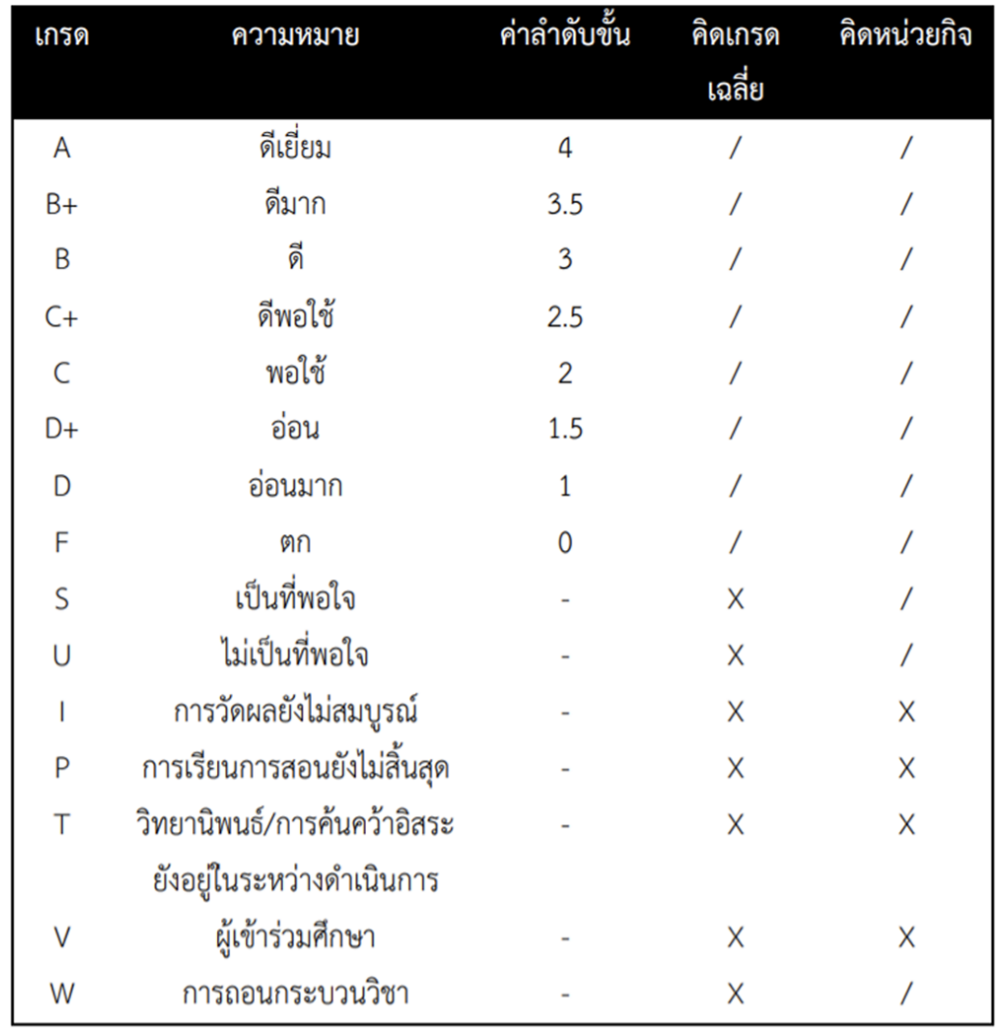
\includegraphics[width=0.8\textwidth]{all_grade.png}
    \caption{grade}
    \label{fig:grade}
  \end{center}
\end{figure}

% \begin{equation}\label{eq:dielectric}
%   k_1=\frac{\omega}{c({1/\varepsilon_m + 1/\varepsilon_i})^{1/2}}=k_2=\frac{\omega
%   \sin(\theta)\varepsilon_\mathit{air}^{1/2}}{c}
%   \end{equation}
% $$GPA=\frac{\sum_{i=1}^{\n}G_i\cdotP_i}{\sum_{i=1}^{\n}P_i}

\section{เกณฑ์มาตรฐานหลักสูตรระดับปริญญาตรี พ.ศ. 2558 ตามประกาศของกระทรวงศึกษาธิการ}
\subsection{โครงสร้างหลักสูตร}
ประกาศของกระทรวงศึกษาธิการฉบับนี้ได้กล่าวถึงโครงสร้างของหลักสูตรในระดับปริญญาตรีไว้ว่า โครงสร้าง
หลักสูตรต้องประกอบด้วยหมวดวิชาศึกษาทั่วไป หมวดวิชาเฉพาะ และหมวดวิชาเลือกเสรี โดยมีสัดส่วนจํานว
นหน่วยกิตของแต่ละหมวดวิชา ดังนี้
\begin{enumerate}
  \item  หมวดวิชาศึกษาทั่วไป หมายถึง หมวดวิชาที่เสริมสร้างความเป็นมนุษย์ที่สมบูรณ์ ให้มีความรอบรู้อย่าง
  กว้างขวาง เข้าใจ และเห็นคุณค่าของตนเอง ผู้อื่น สังคม ศิลปวัฒนธรรม และธรรมชาติ ใส่ใจต่อความ
  เปลี่ยนแปลงของสรรพสิ่ง พัฒนาตนเองอย่างต่อเนื่อง ดําเนินชีวิตอย่างมีคุณธรรม พร้อมให้ความช่วย
  เหลือเพื่อนมนุษย์ และเป็นพลเมืองที่มีคุณค่าของสังคมไทยและสังคมโลก
  สถาบันอุดมศึกษาอาจจัดวิชาศึกษาทั่วไปในลักษณะจําแนกเป็นรายวิชาหรือลักษณะบูรณาการใด ๆ
  ก็ได้ โดยผสมผสานเนื้อหาวิชาที่ครอบคลุมสาระของกลุ่มวิชาสังคมศาสตร์ มนุษยศาสตร์ ภาษาและ
  กลุ่มวิชาวิทยาศาสตร์กับคณิตศาสตร์ ในสัดส่วนที่เหมาะสม เพื่อให้บรรลุวัตถุประสงค์ของ หมวดวิชา
  ศึกษาทั่วไป โดยให้มีจํานวนหน่วยกิตรวมไม่น้อยกว่า 30 หน่วยกิต
  อนึ่ง การจัดวิชาศึกษาทั่วไปสําหรับหลักสูตรปริญญาตรี(ต่อเนื่อง) อาจได้รับการยกเว้นรายวิชาที่ได้
  ศึกษามาแล้วในระดับประกาศนียบัตรวิชาชีพชั้นสูงหรือระดับอนุปริญญา ทั้งนี้ จํานวนหน่วยกิตของ
  รายวิชาที่ได้รับการยกเว้นดังกล่าว เมื่อนับรวมกับรายวิชาที่จะศึกษาเพิ่มเติมในหลักสูตรปริญญาตรี
  (ต่อเนื่อง) ต้องไม่น้อยกว่า 30 หน่วยกิต
  \item หมวดวิชาเฉพาะ หมายถึง วิชาแกน วิชาเฉพาะด้าน วิชาพื้นฐานวิชาชีพและวิชาชีพ ที่มุ่งหมายให้ผู้
  เรียนมีความรู้ ความเข้าใจ และปฏิบัติงานได้ โดยให้มีจํานวนหน่วยกิตรวม ดังนี้
  \begin{itemize}
    \item หลักสูตรปริญญาตรี(4 ปี) ทางวิชาการ ให้มีจํานวนหน่วยกิตหมวดวิชาเฉพาะ รวมไม่น้อยกว่า
    72 หน่วยกิต
    \item หลักสูตรปริญญาตรี(4 ปี) ทางวิชาชีพหรือปฏิบัติการ ให้มีจํานวน หน่วยกิตหมวดวิชาเฉพาะ
    รวมไม่น้อยกว่า 72 หน่วยกิต โดยต้องเรียนวิชาทางปฏิบัติการตามที่ มาตรฐานวิชาชีพกําหนด
    หากไม่มีมาตรฐานวิชาชีพกําหนดต้องเรียนวิชาทางปฏิบัติการไม่น้อยกว่า 36 หน่วยกิต และ
    ทางทฤษฎีไม่น้อยกว่า 24 หน่วยกิต
    \item หลักสูตร (ต่อเนื่อง) ให้มีจํานวนหน่วยกิตหมวดวิชาเฉพาะรวมไม่น้อยกว่า 42 หน่วยกิต ในจํา
    นวนนั้นต้องเป็นวิชาทางทฤษฏีไม่น้อยกว่า 18 หน่วยกิต
    \item หลักสูตรปริญญาตรี(5 ปี) ให้มีจํานวนหน่วยกิตหมวดวิชาเฉพาะรวม ไม่น้อยกว่า 90 หน่วยกิต
    \item  หลักสูตรปริญญาตรี(ไม่น้อยกว่า 6 ปี) ให้มีจํานวนหน่วยกิตหมวดวิชา เฉพาะรวมไม่น้อยกว่า
    108 หน่วยกิต
 \end{itemize}
 สถาบันอุดมศึกษาอาจจัดหมวดวิชาเฉพาะในลักษณะวิชาเอกเดี่ยว วิชาเอกคู่ หรือวิชาเอกและวิชาโท
ก็ได้ โดยวิชาเอกต้องมีจํานวนหน่วยกิตไม่น้อยกว่า 30 หน่วยกิต และวิชาโทต้องมีจํานวนหน่วยกิตไม่
น้อยกว่า 15 หน่วยกิต ในกรณีที่จัดหลักสูตรแบบวิชาเอกคู่ต้องเพิ่ม จํานวนหน่วยกิตของวิชาเอกอีก
ไม่น้อยกว่า 30 หน่วยกิต และให้มีจํานวนหน่วยกิตรวมไม่น้อยกว่า 150 หน่วยกิต
สําหรับหลักสูตรปริญญาตรีแบบก้าวหน้า ผู้เรียนต้องเรียนวิชาระดับบัณฑิตศึกษาในหมวดวิชาเฉพาะ
ไม่น้อยกว่า 12 หน่วยกิต
\item  หมวดวิชาเลือกเสรี หมายถึง วิชาที่มุ่งให้ผู้เรียนมีความรู้ ความเข้าใจ ตามที่ ตนเองถนัดหรือสนใจ โดย
เปิดโอกาสให้ผู้เรียนเลือกเรียนรายวิชาใด ๆ ในหลักสูตรระดับปริญญาตรี โดยให้มีจํานวนหน่วยกิต
รวมไม่น้อยกว่า 6 หน่วยกิต สถาบันอุดมศึกษาอาจยกเว้นหรือเทียบโอนหน่วยกิตรายวิชาในหมวดวิชาศึกษาทั่วไป หมวดวิชาเฉพาะ
และหมวดวิชาเลือกเสรี ให้กับนักศึกษาที่มีความรู้ความสามารถ ที่สามารถวัดมาตรฐานได้ ทั้งนี้ นักศึกษาต้องศึกษาให้ครบตามจํานวนหน่วยกิตที่กําหนดไว้ในเกณฑ์มาตรฐานหลักสูตร และเป็นไป ตาม
หลักเกณฑ์การเทียบโอนผลการเรียนระดับปริญญาเข้าสู่การศึกษาในระบบ และแนวปฏิบัติที่ดี เกี่ยว
กับการเทียบโอน ของสํานักงานคณะกรรมการการอุดมศึกษา
\end{enumerate}
\subsection{เกณฑ์การวัดผลและการสําเร็จการศึกษา}
ให้สถาบันอุดมศึกษากําหนดเกณฑ์การวัดผล เกณฑ์ขั้นต่ําของแต่ละรายวิชา และเกณฑ์การสําเร็จการศึกษา
ตามหลักสูตร โดยต้องเรียนครบ ตามจํานวนหน่วยกิตที่กําหนดไว้ในหลักสูตร และต้องได้ระดับคะแนนเฉลี่ย
ไม่ตํ่ากว่า 2.00 จากระบบ 4 ระดับคะแนนหรือเทียบเท่า จึงถือว่าเรียนจบหลักสูตรปริญญาตรี

\chapter{\ifproject%
\ifenglish Project Structure and Methodology\else โครงสร้างและขั้นตอนการทำงาน\fi
\else%
\ifenglish Project Structure\else โครงสร้างของโครงงาน\fi
\fi
}

\makeatletter

% \renewcommand\section{\@startsection {section}{1}{\z@}%
%                                    {13.5ex \@plus -1ex \@minus -.2ex}%
%                                    {2.3ex \@plus.2ex}%
%                                    {\normalfont\large\bfseries}}

\makeatother
%\vspace{2ex}
% \titleformat{\section}{\normalfont\bfseries}{\thesection}{1em}{}
% \titlespacing*{\section}{0pt}{10ex}{0pt}

\section{โครงสร้างของระบบ}
\subsection{หน้าเว็บสำหรับนักศึกษา}
\begin{center}
สำหรับนักศึกษา จะต้องล็อคอินผ่าน CMU Account ของมหาวิทยาลัยเพื่อที่จะสามารถเข้าสู่ระบบได้
\end{center}

\begin{figure}[H]
  \begin{center}
    \subfigure{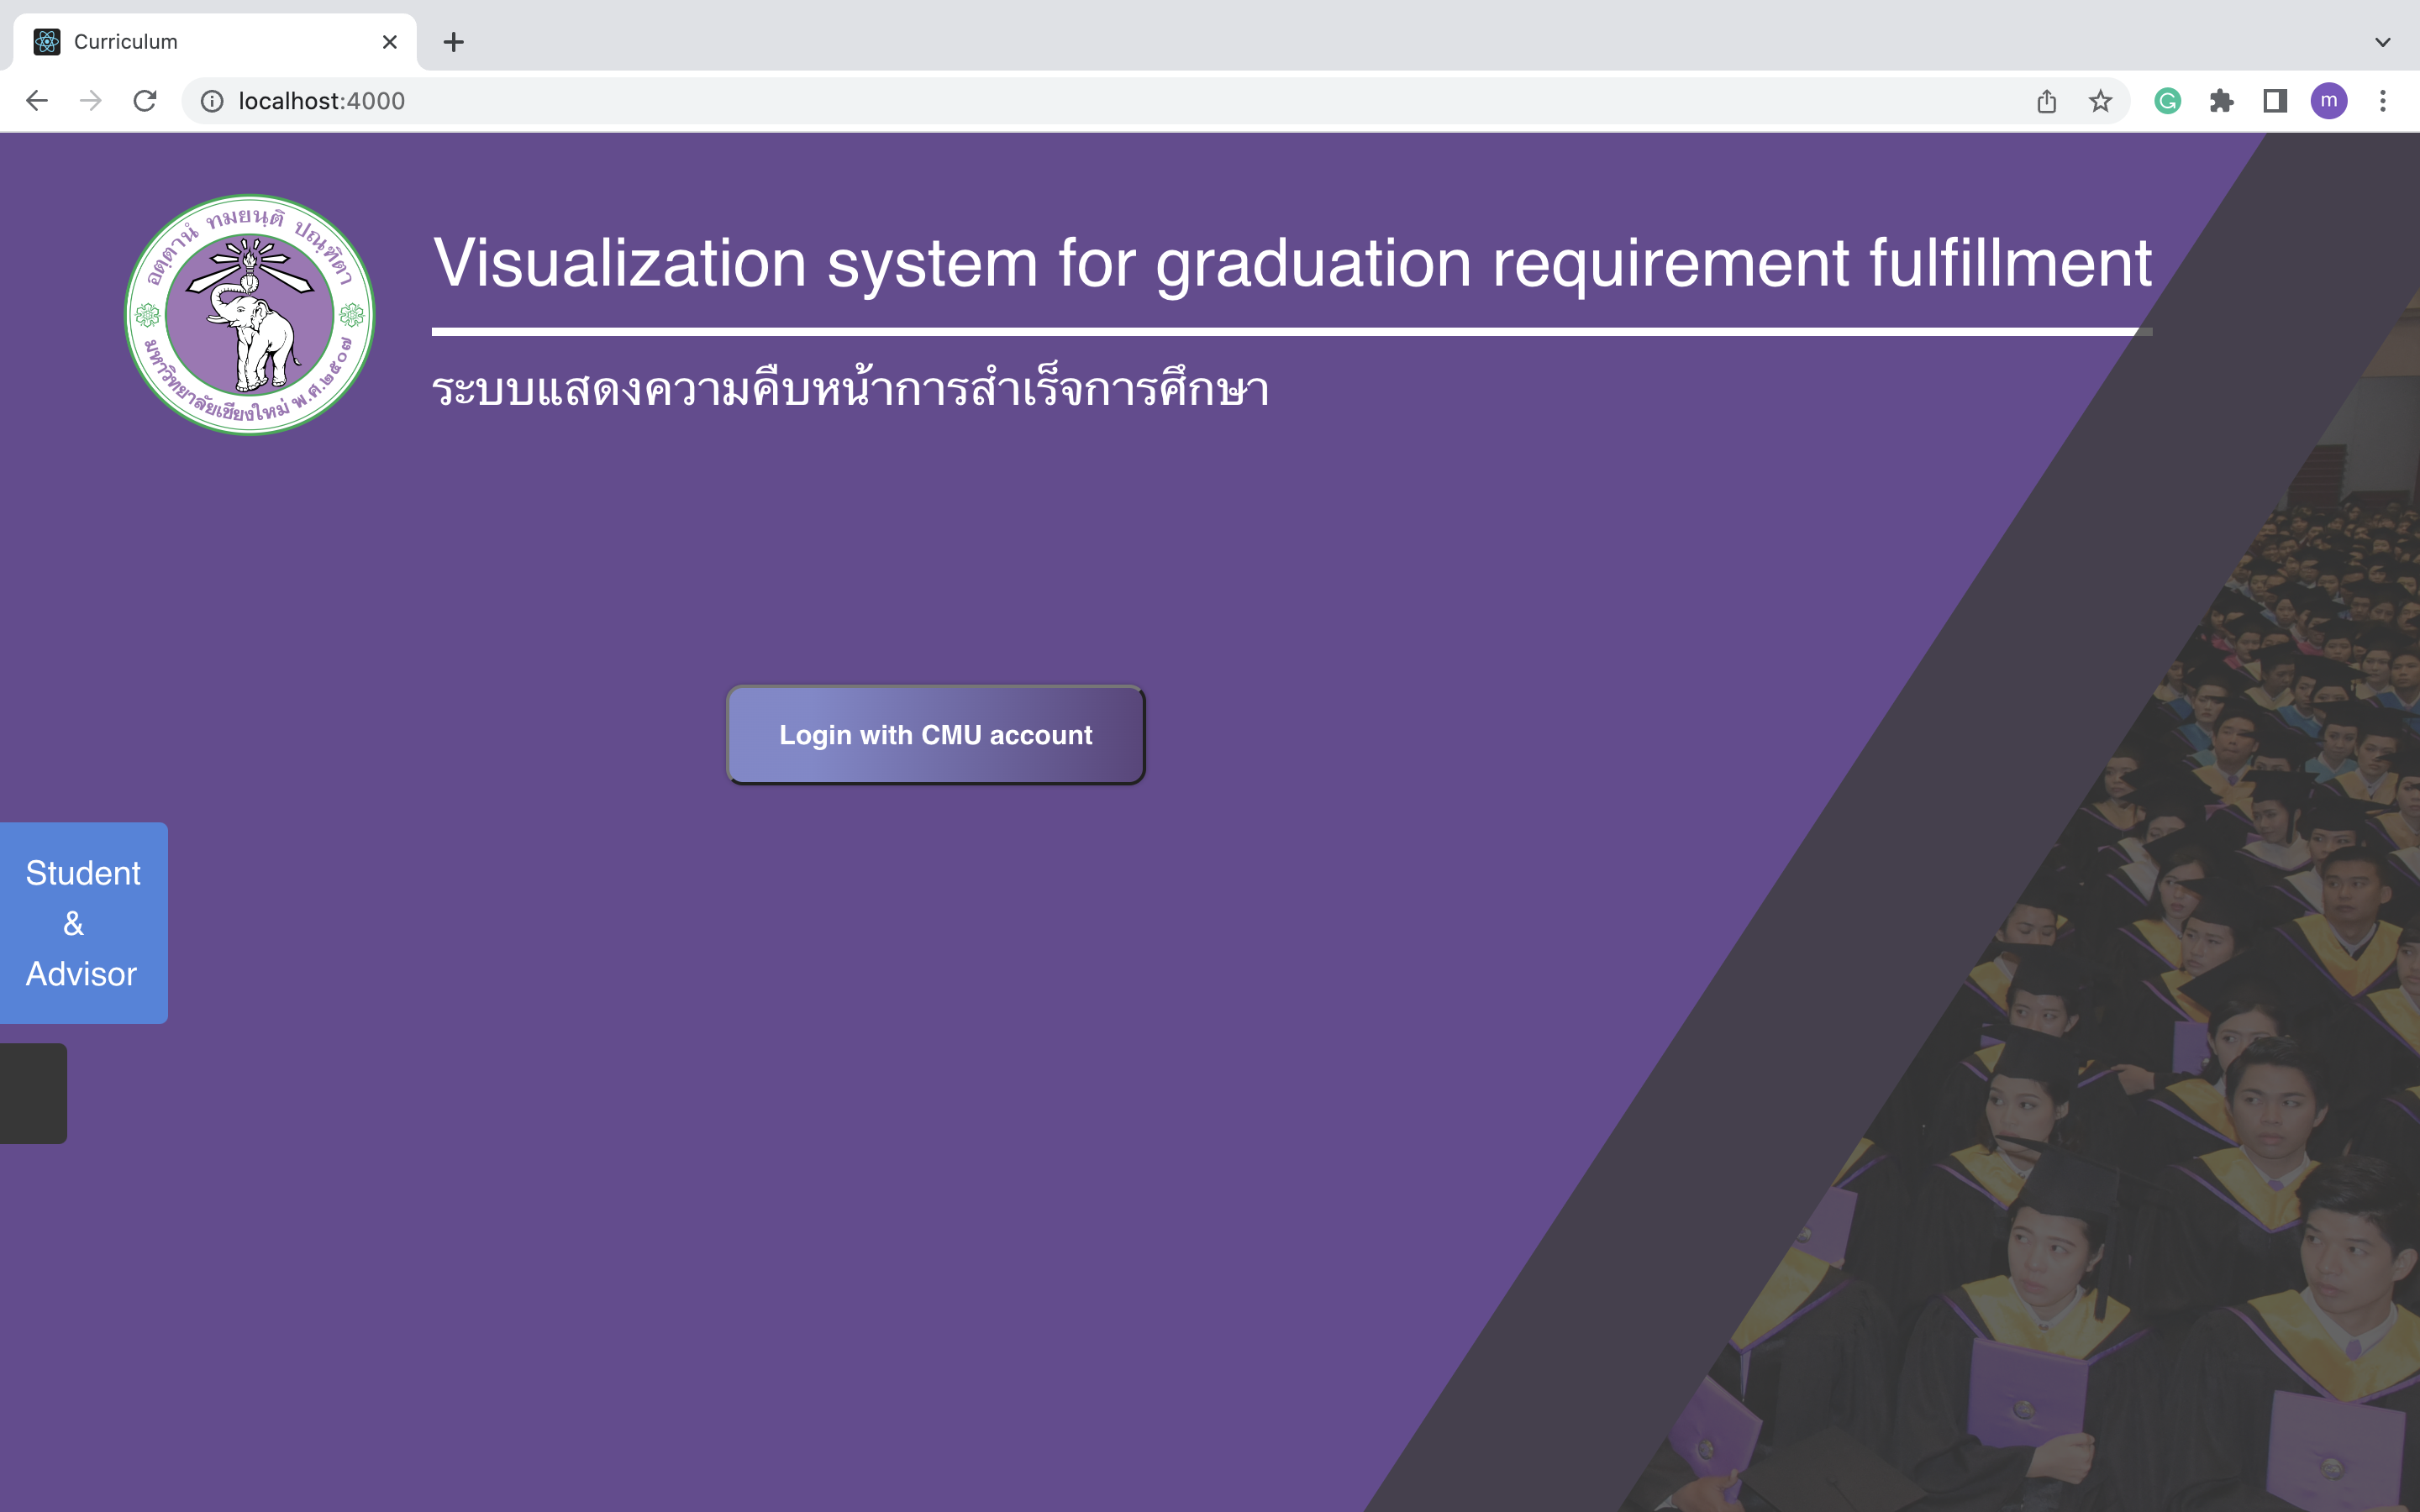
\includegraphics[width=0.8\textwidth]{login.png}}
    \subfigure{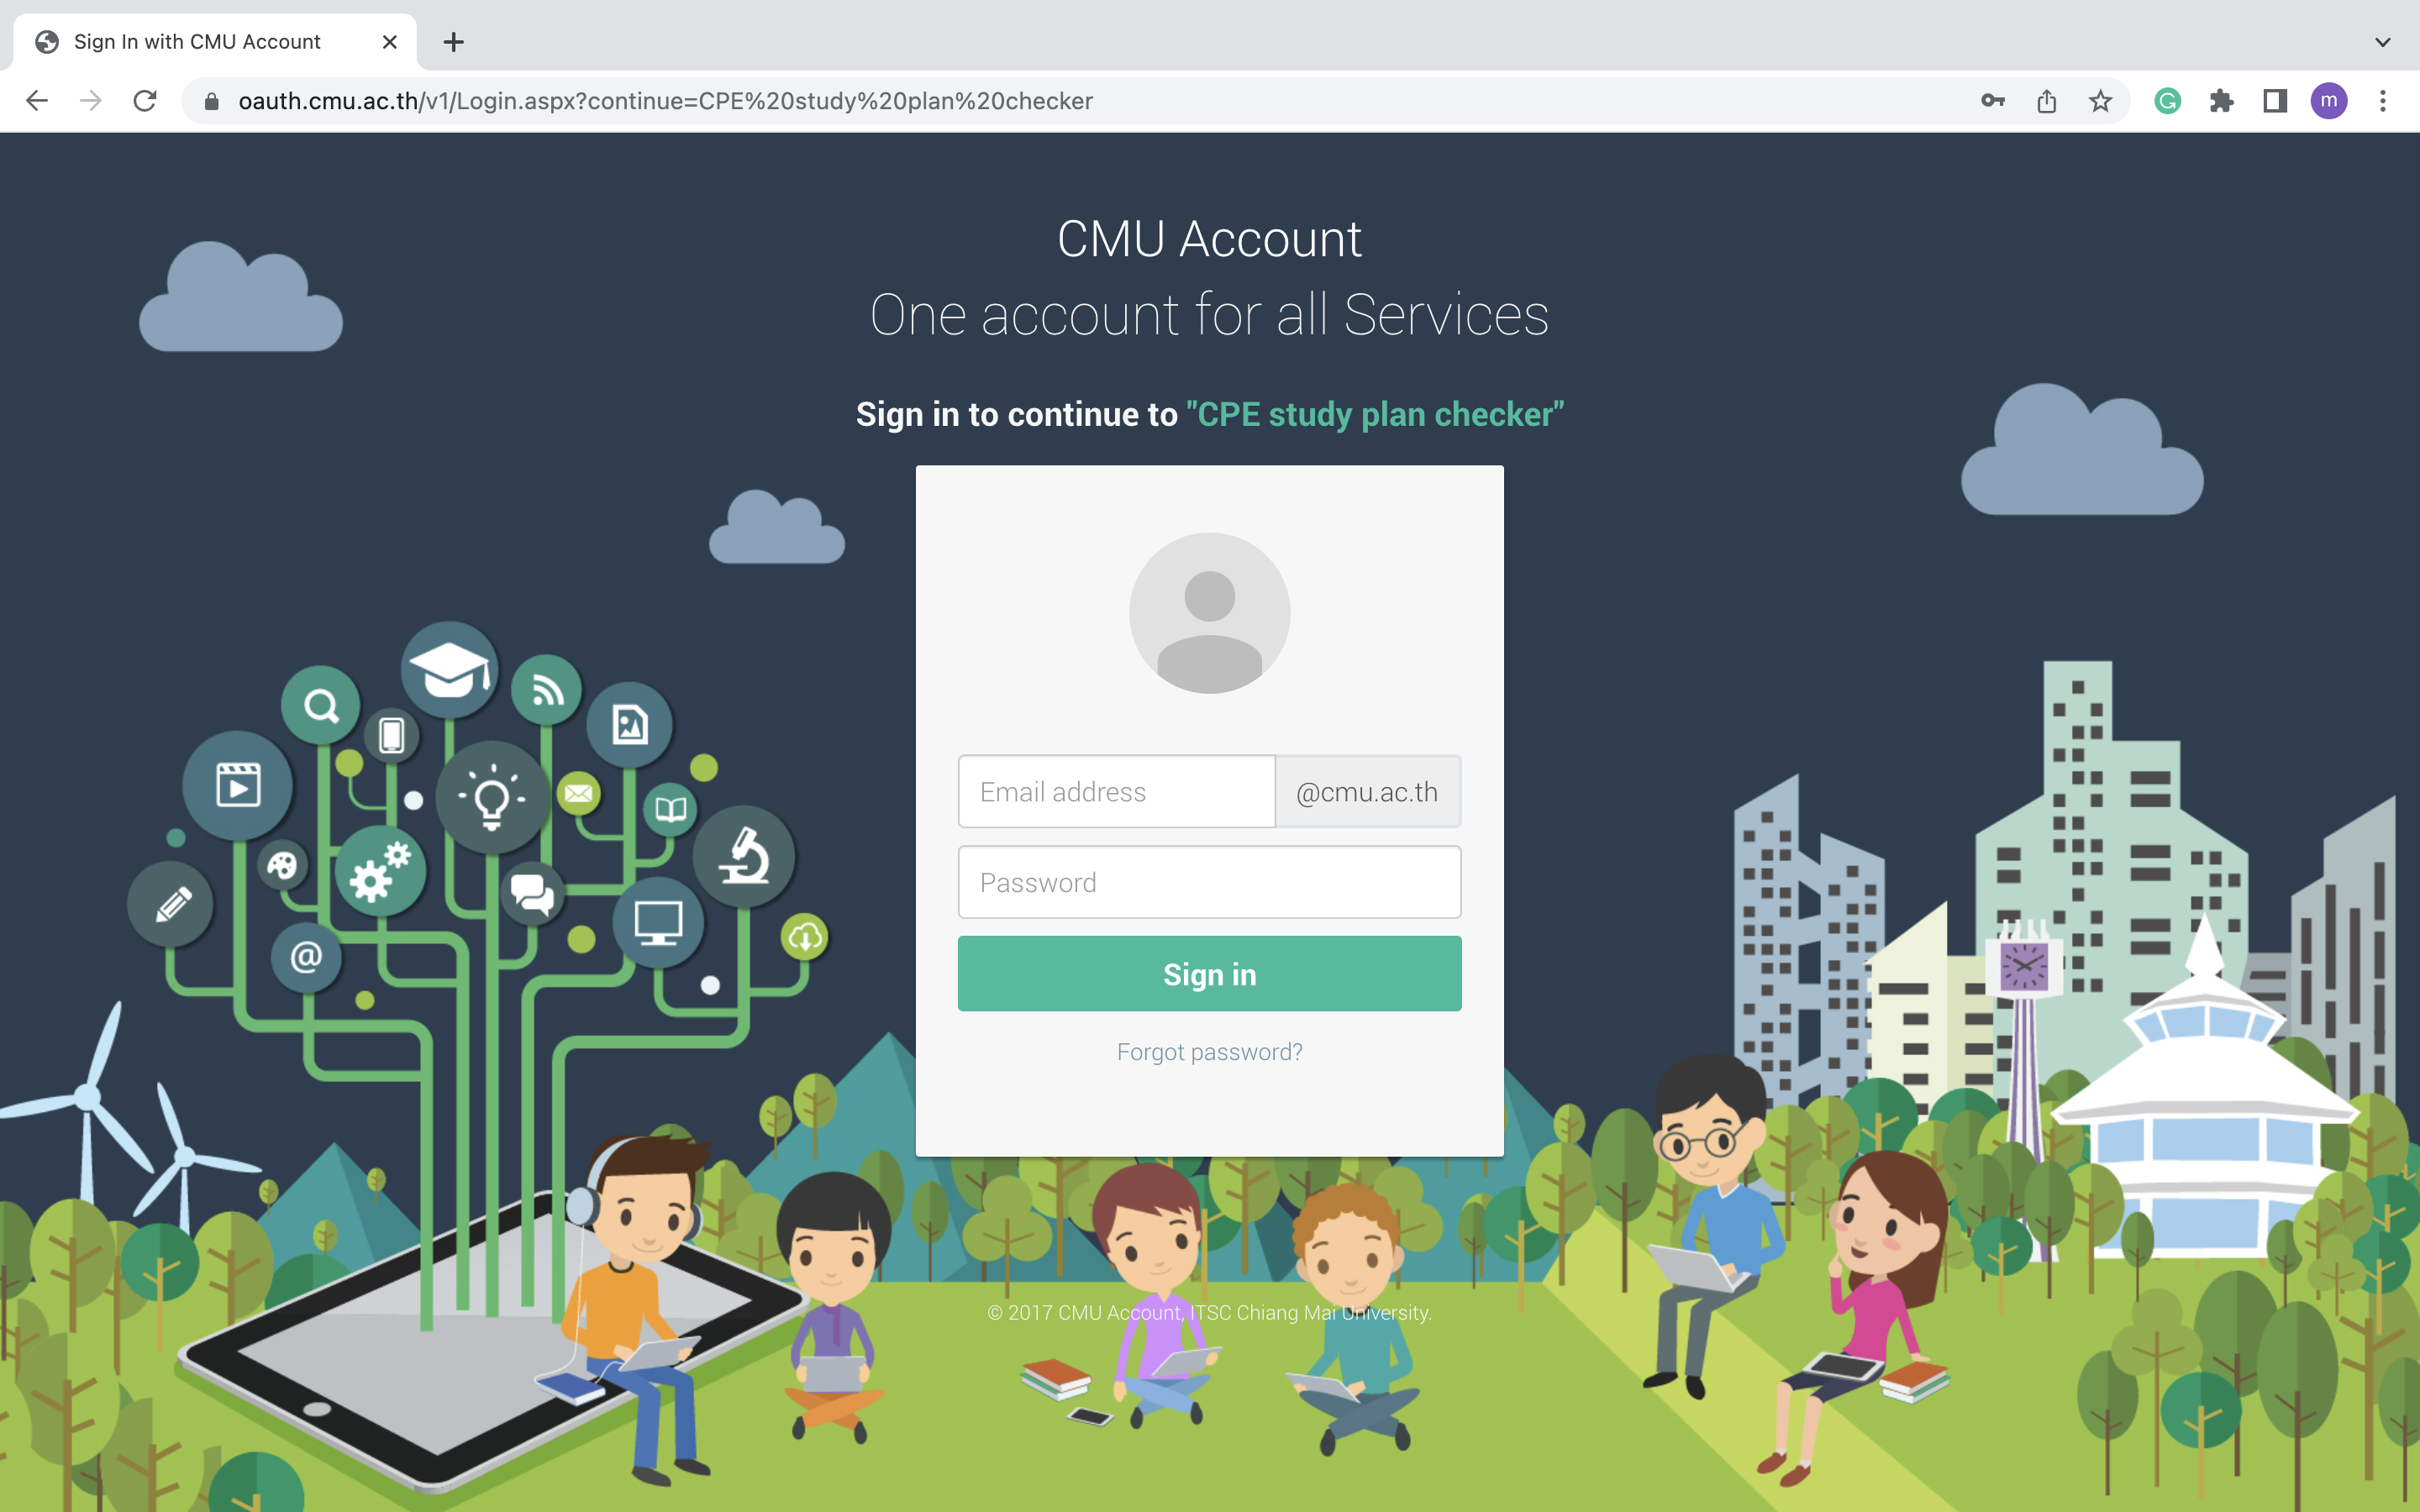
\includegraphics[width=0.8\textwidth]{oauth.png}}
  \end{center}
  \caption{หน้า Student Login}
  \label{fig:login}
\end{figure}

% \begin{center}
%   ตัวเลือกแผนการเรียน
% \end{center}

\begin{figure}[H]
  \begin{center}
    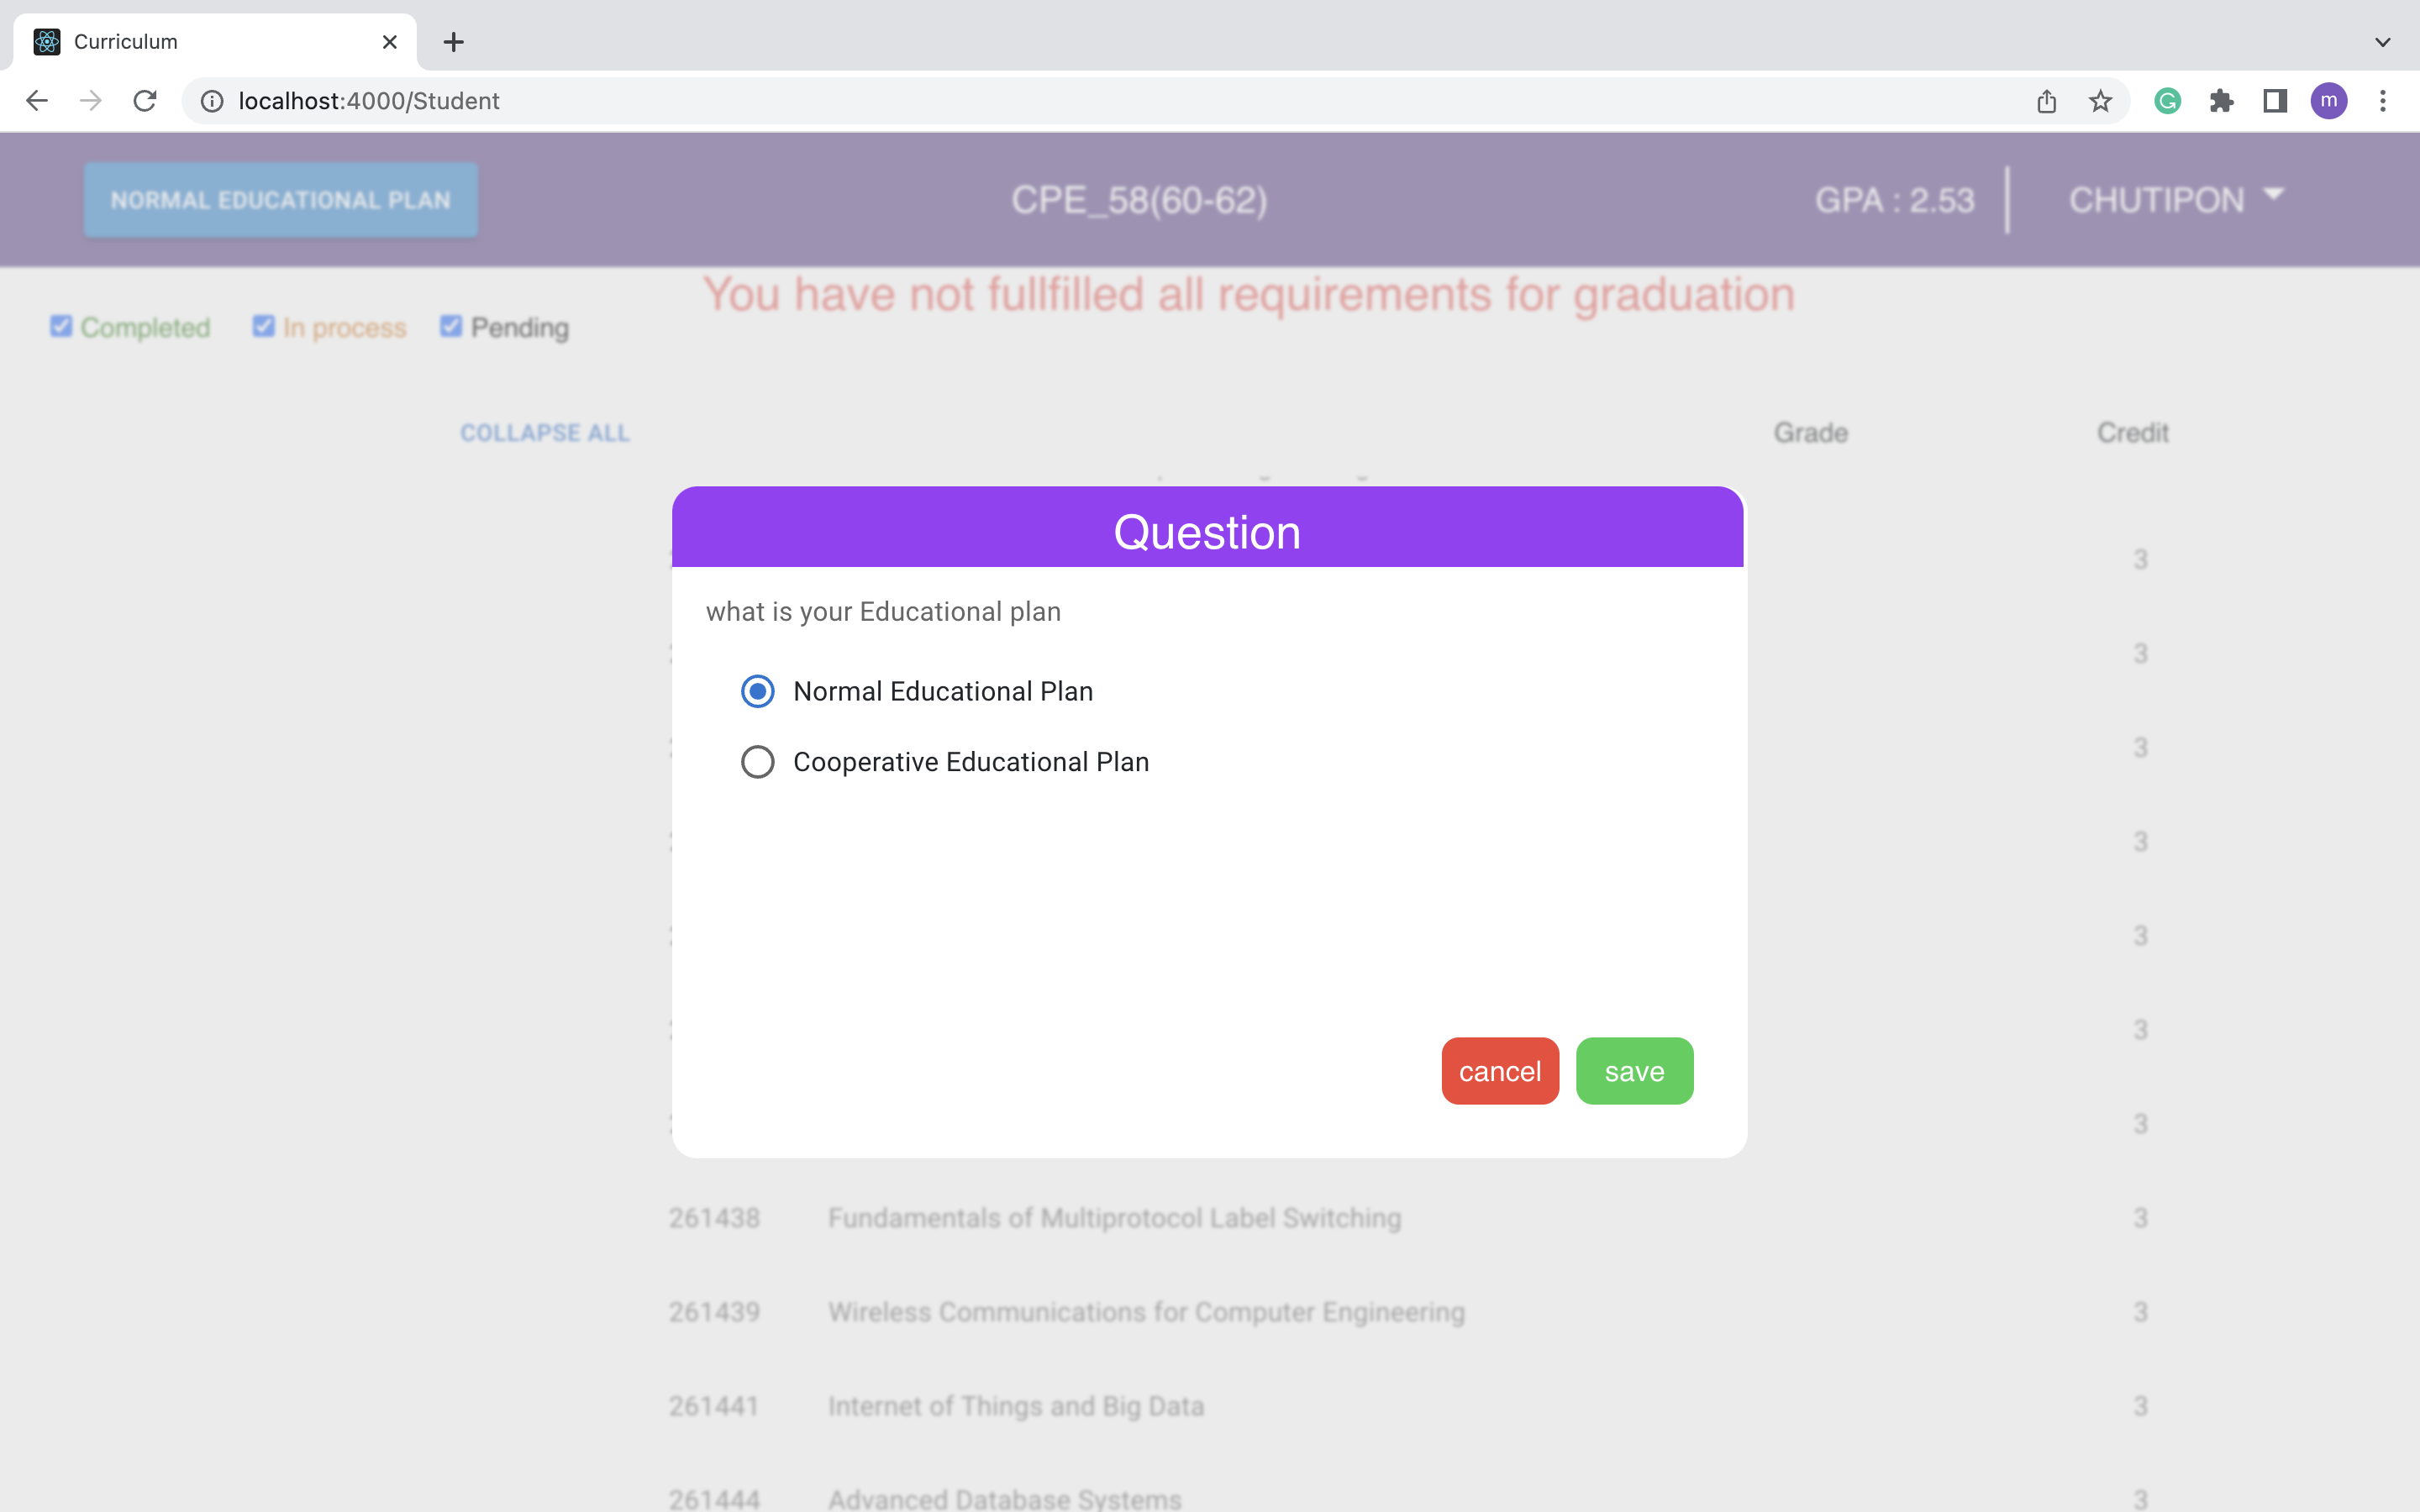
\includegraphics[width=0.8\textwidth]{question.png}
    \caption{หน้าเลือกเเผนการศึกษา}
    \label{fig:question}
  \end{center}
\end{figure}

\begin{figure}[H]
  \begin{center}
    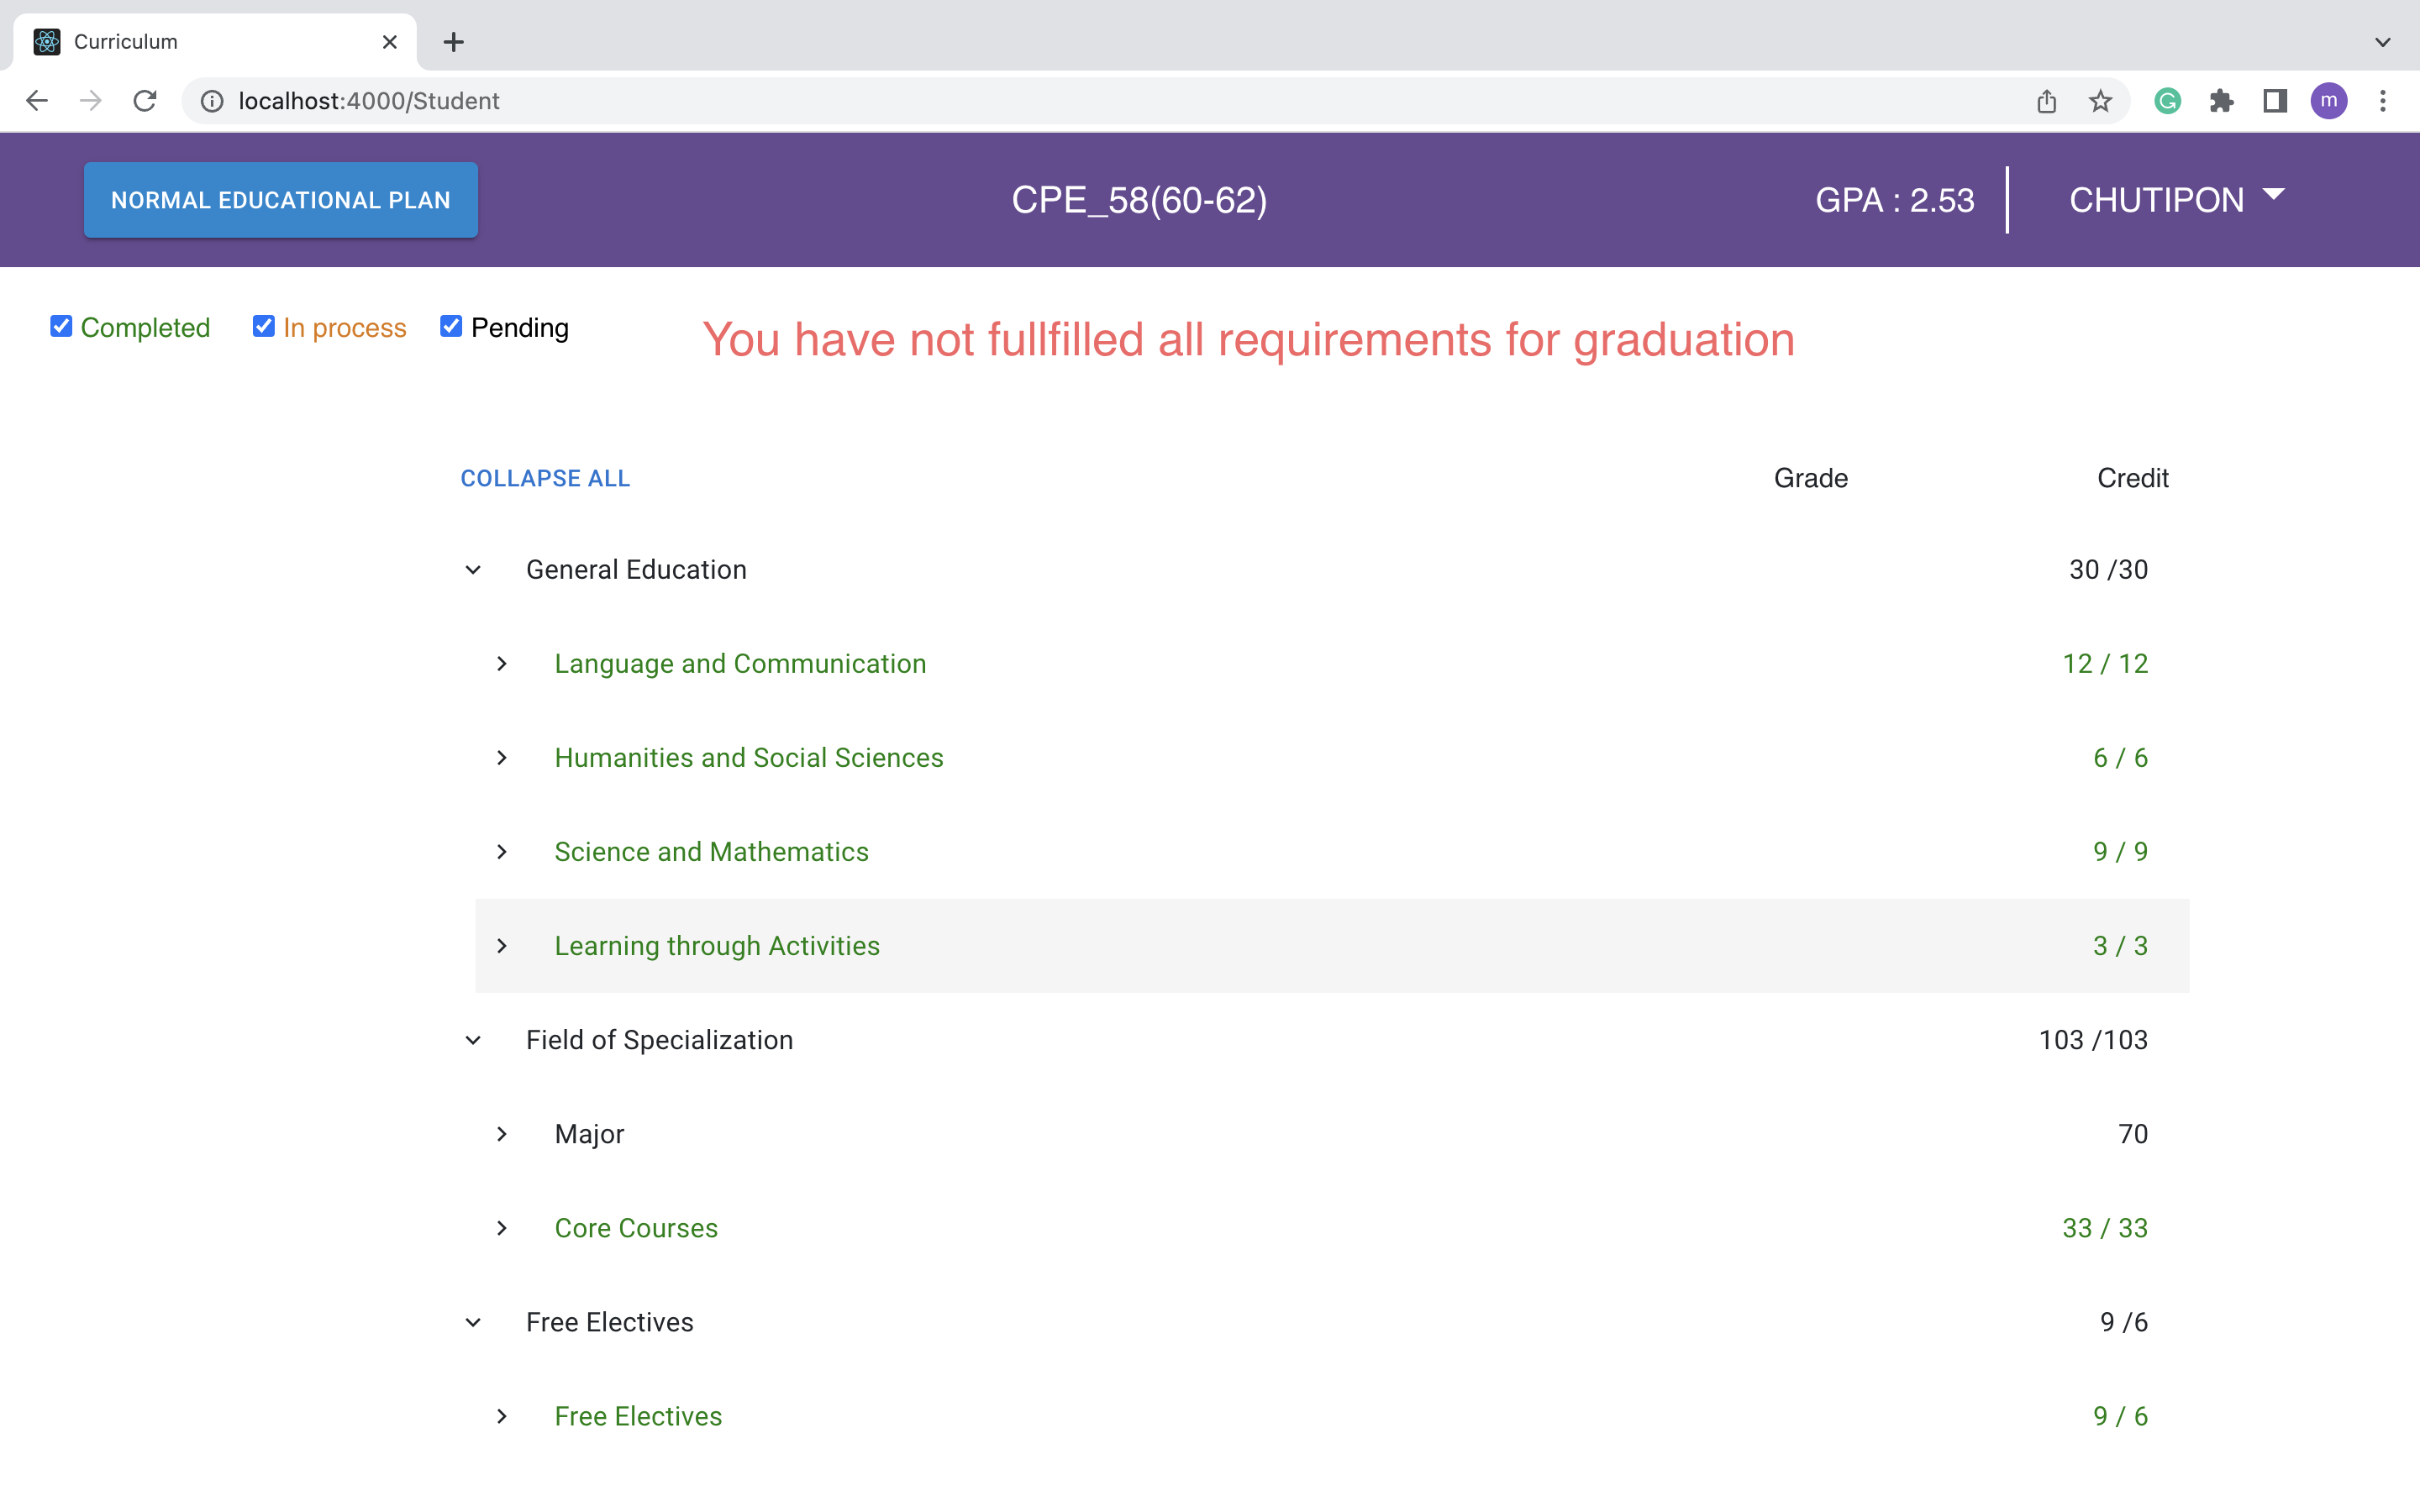
\includegraphics[width=0.8\textwidth]{student.png}
    \caption{หน้าเเสดงผลการศึกษา}
    \label{fig:student}
  \end{center}
\end{figure}

การใช้งานของนักศึกษา เมื่อเข้าสู่ระบบเป็นที่เรียบร้อยแล้วนั้น นักศึกษาจะเห็นโครงสร้างหลักสูตรของตนเองที่จะอธิบาย
รายวิชาในหมวดต่างๆ ได้แก่รายวิชาที่เรียนสำเร็จแล้ว (สถานะสีเขียวพร้อมเกรดที่ได้รับ) รายวิชาที่กำลังลงเรียนอยู่ในเทอมนั้น
(สถานะสีนํ้าตาล) และรายวิชาที่ยังไม่ได้ลงทะเบียนเรียนหรือเป็นวิชาที่ไม่ผ่านจากเทอมที่ผ่านมาและไม่ได้ลงเรียนอยู่ในเทอมนั้น (สถานะ
เเดง เเละเทา) ซึ่งนักศึกษาสามารถเลือกดูเพียงสถานะที่ตนเองสนใจได้โดยการเลือกฟังก์ชันเช็คบล็อค เพื่อแสดงสถานะที่มุมบนซ้ายมือของเว็บ
เพจ นอกจากนี้นักศึกษาสามารถเลือกแผนการเรียนและความถนัดในสาขาวิชาชีพของตนเองตามที่หลักสูตรกำหนดไว้ โดยการเลือกที่
ฟังก์ชันคำถามแล้วตอบคำถามตามที่ตนเองสนใจ

% \begin{figure}[b]
%   \begin{center}
%     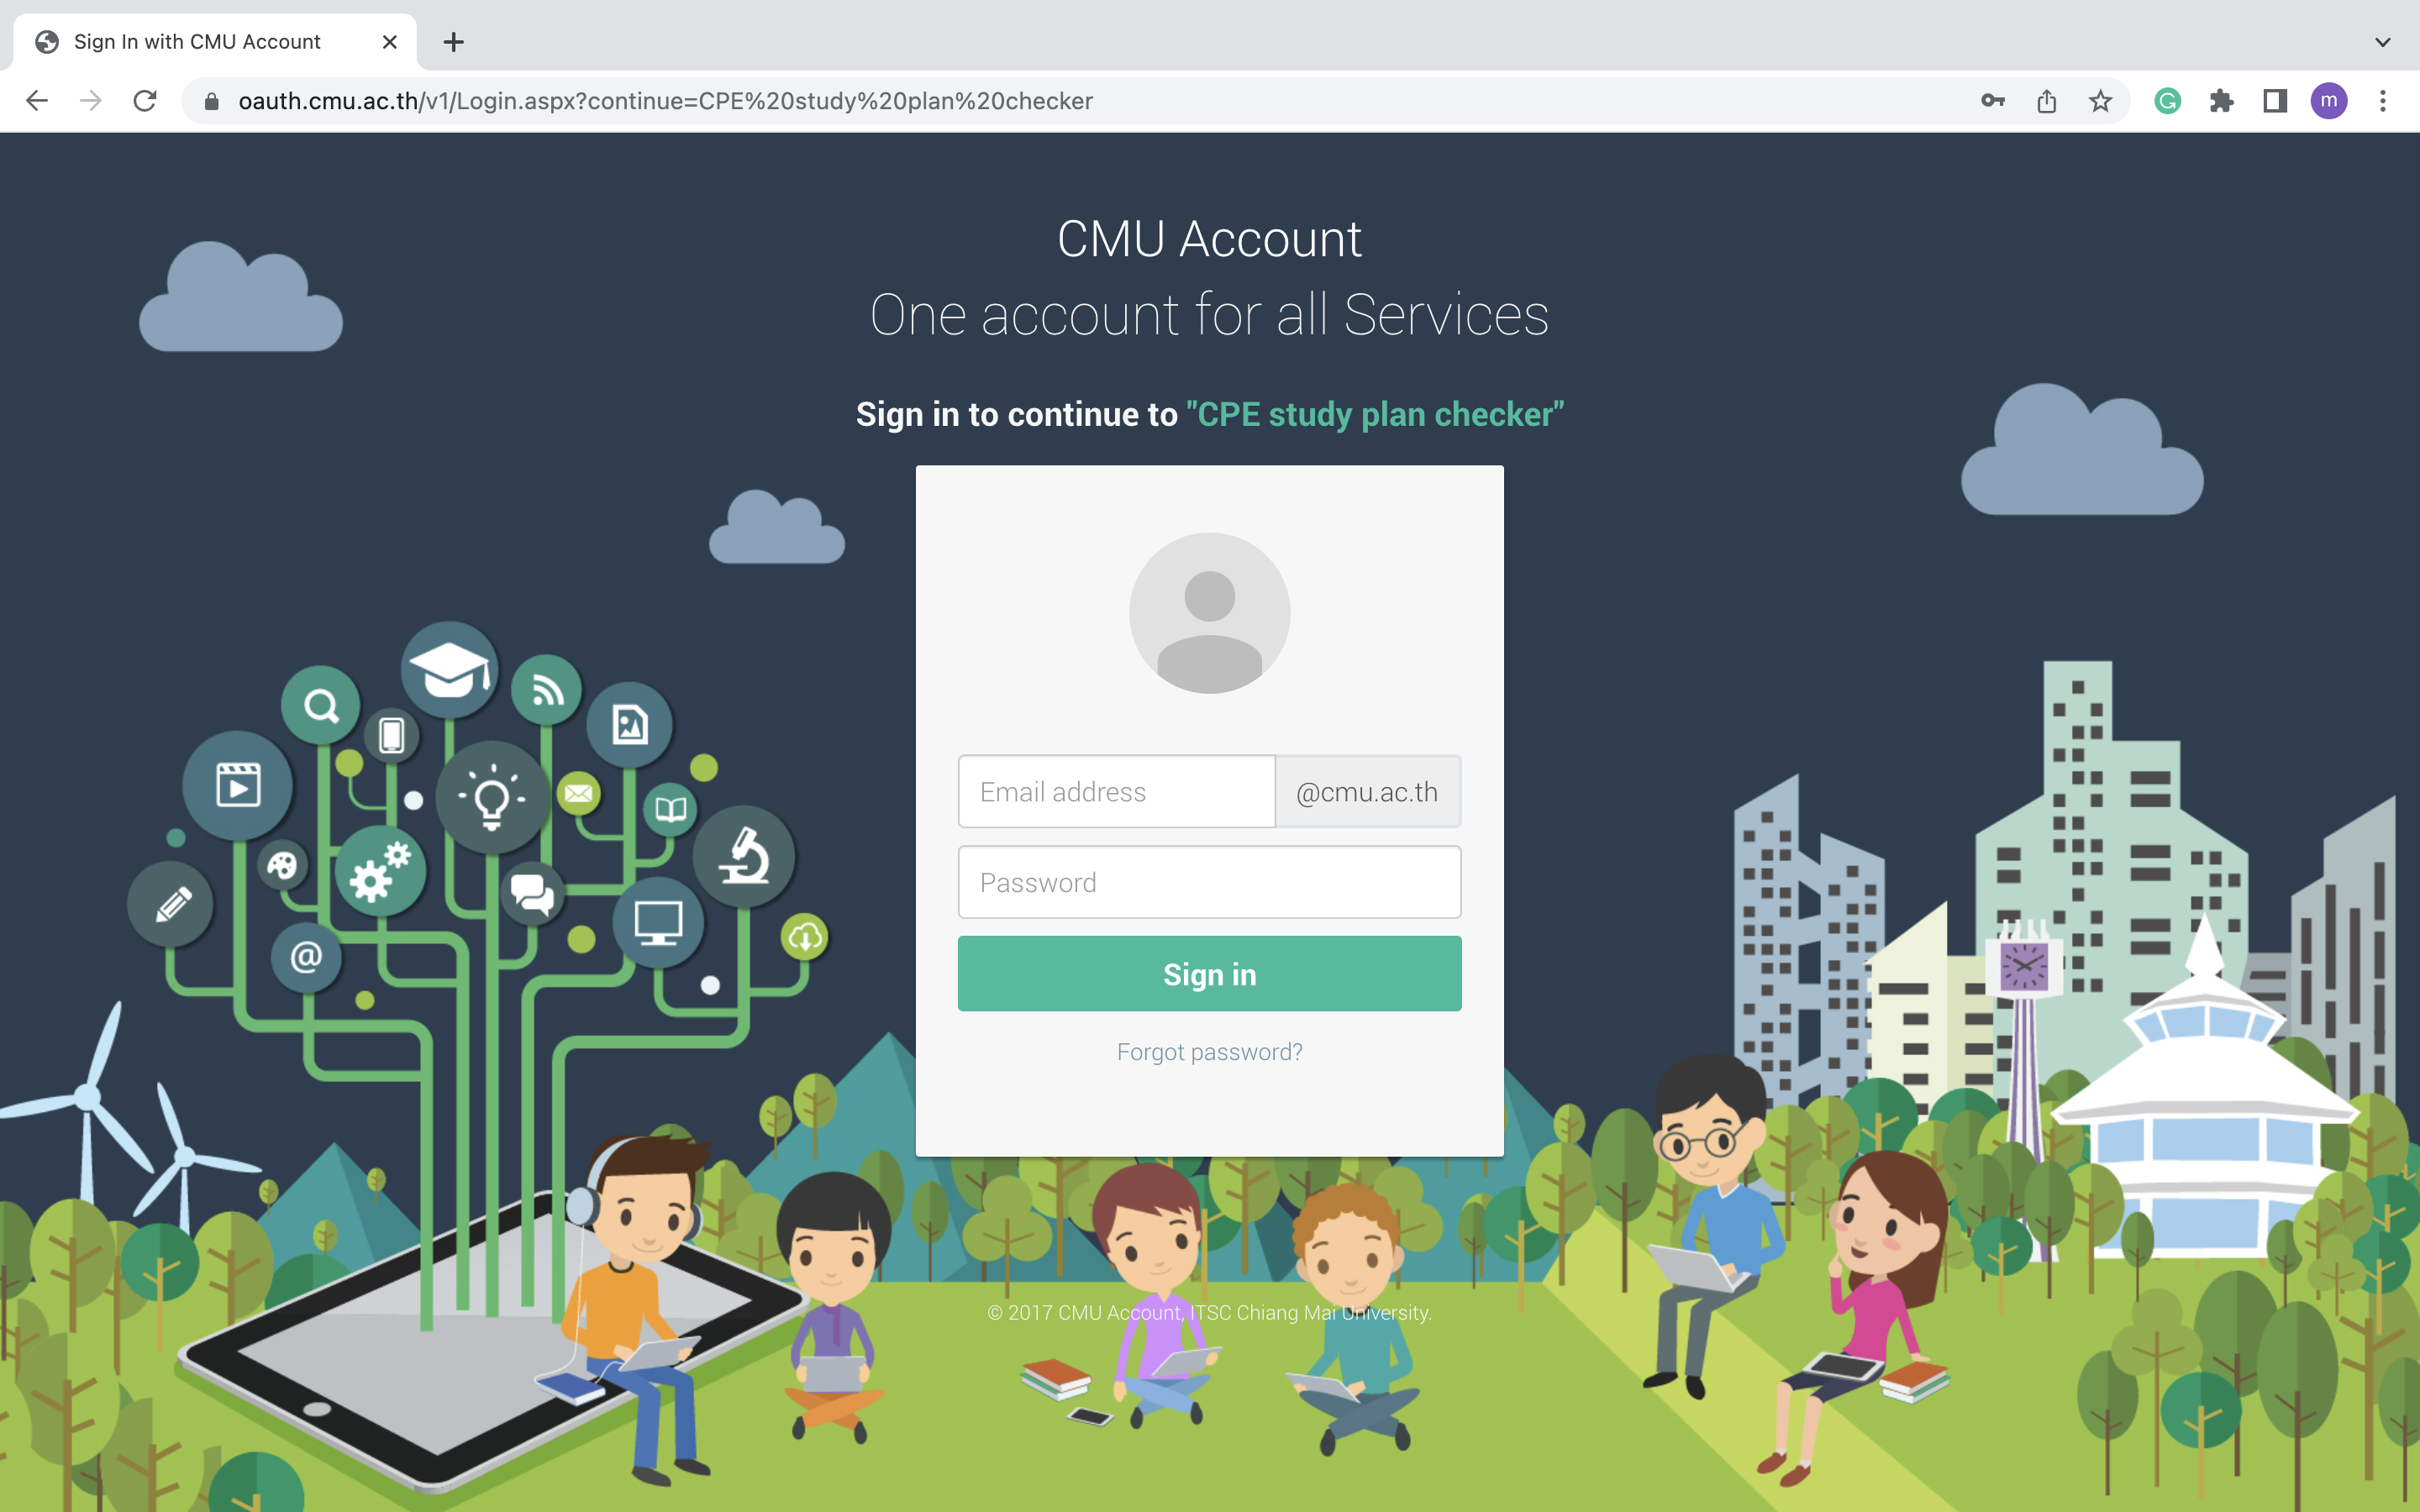
\includegraphics[width=0.8\textwidth]{oauth.png}
%     \caption{หน้า OAuth login}
%     \label{fig:oauth}
%   \end{center}
% \end{figure}

\subsection{หน้าเว็บสำหรับอาจารย์ที่ปรึกษา}

\begin{figure}[H]
  \begin{center}
    \subfigure{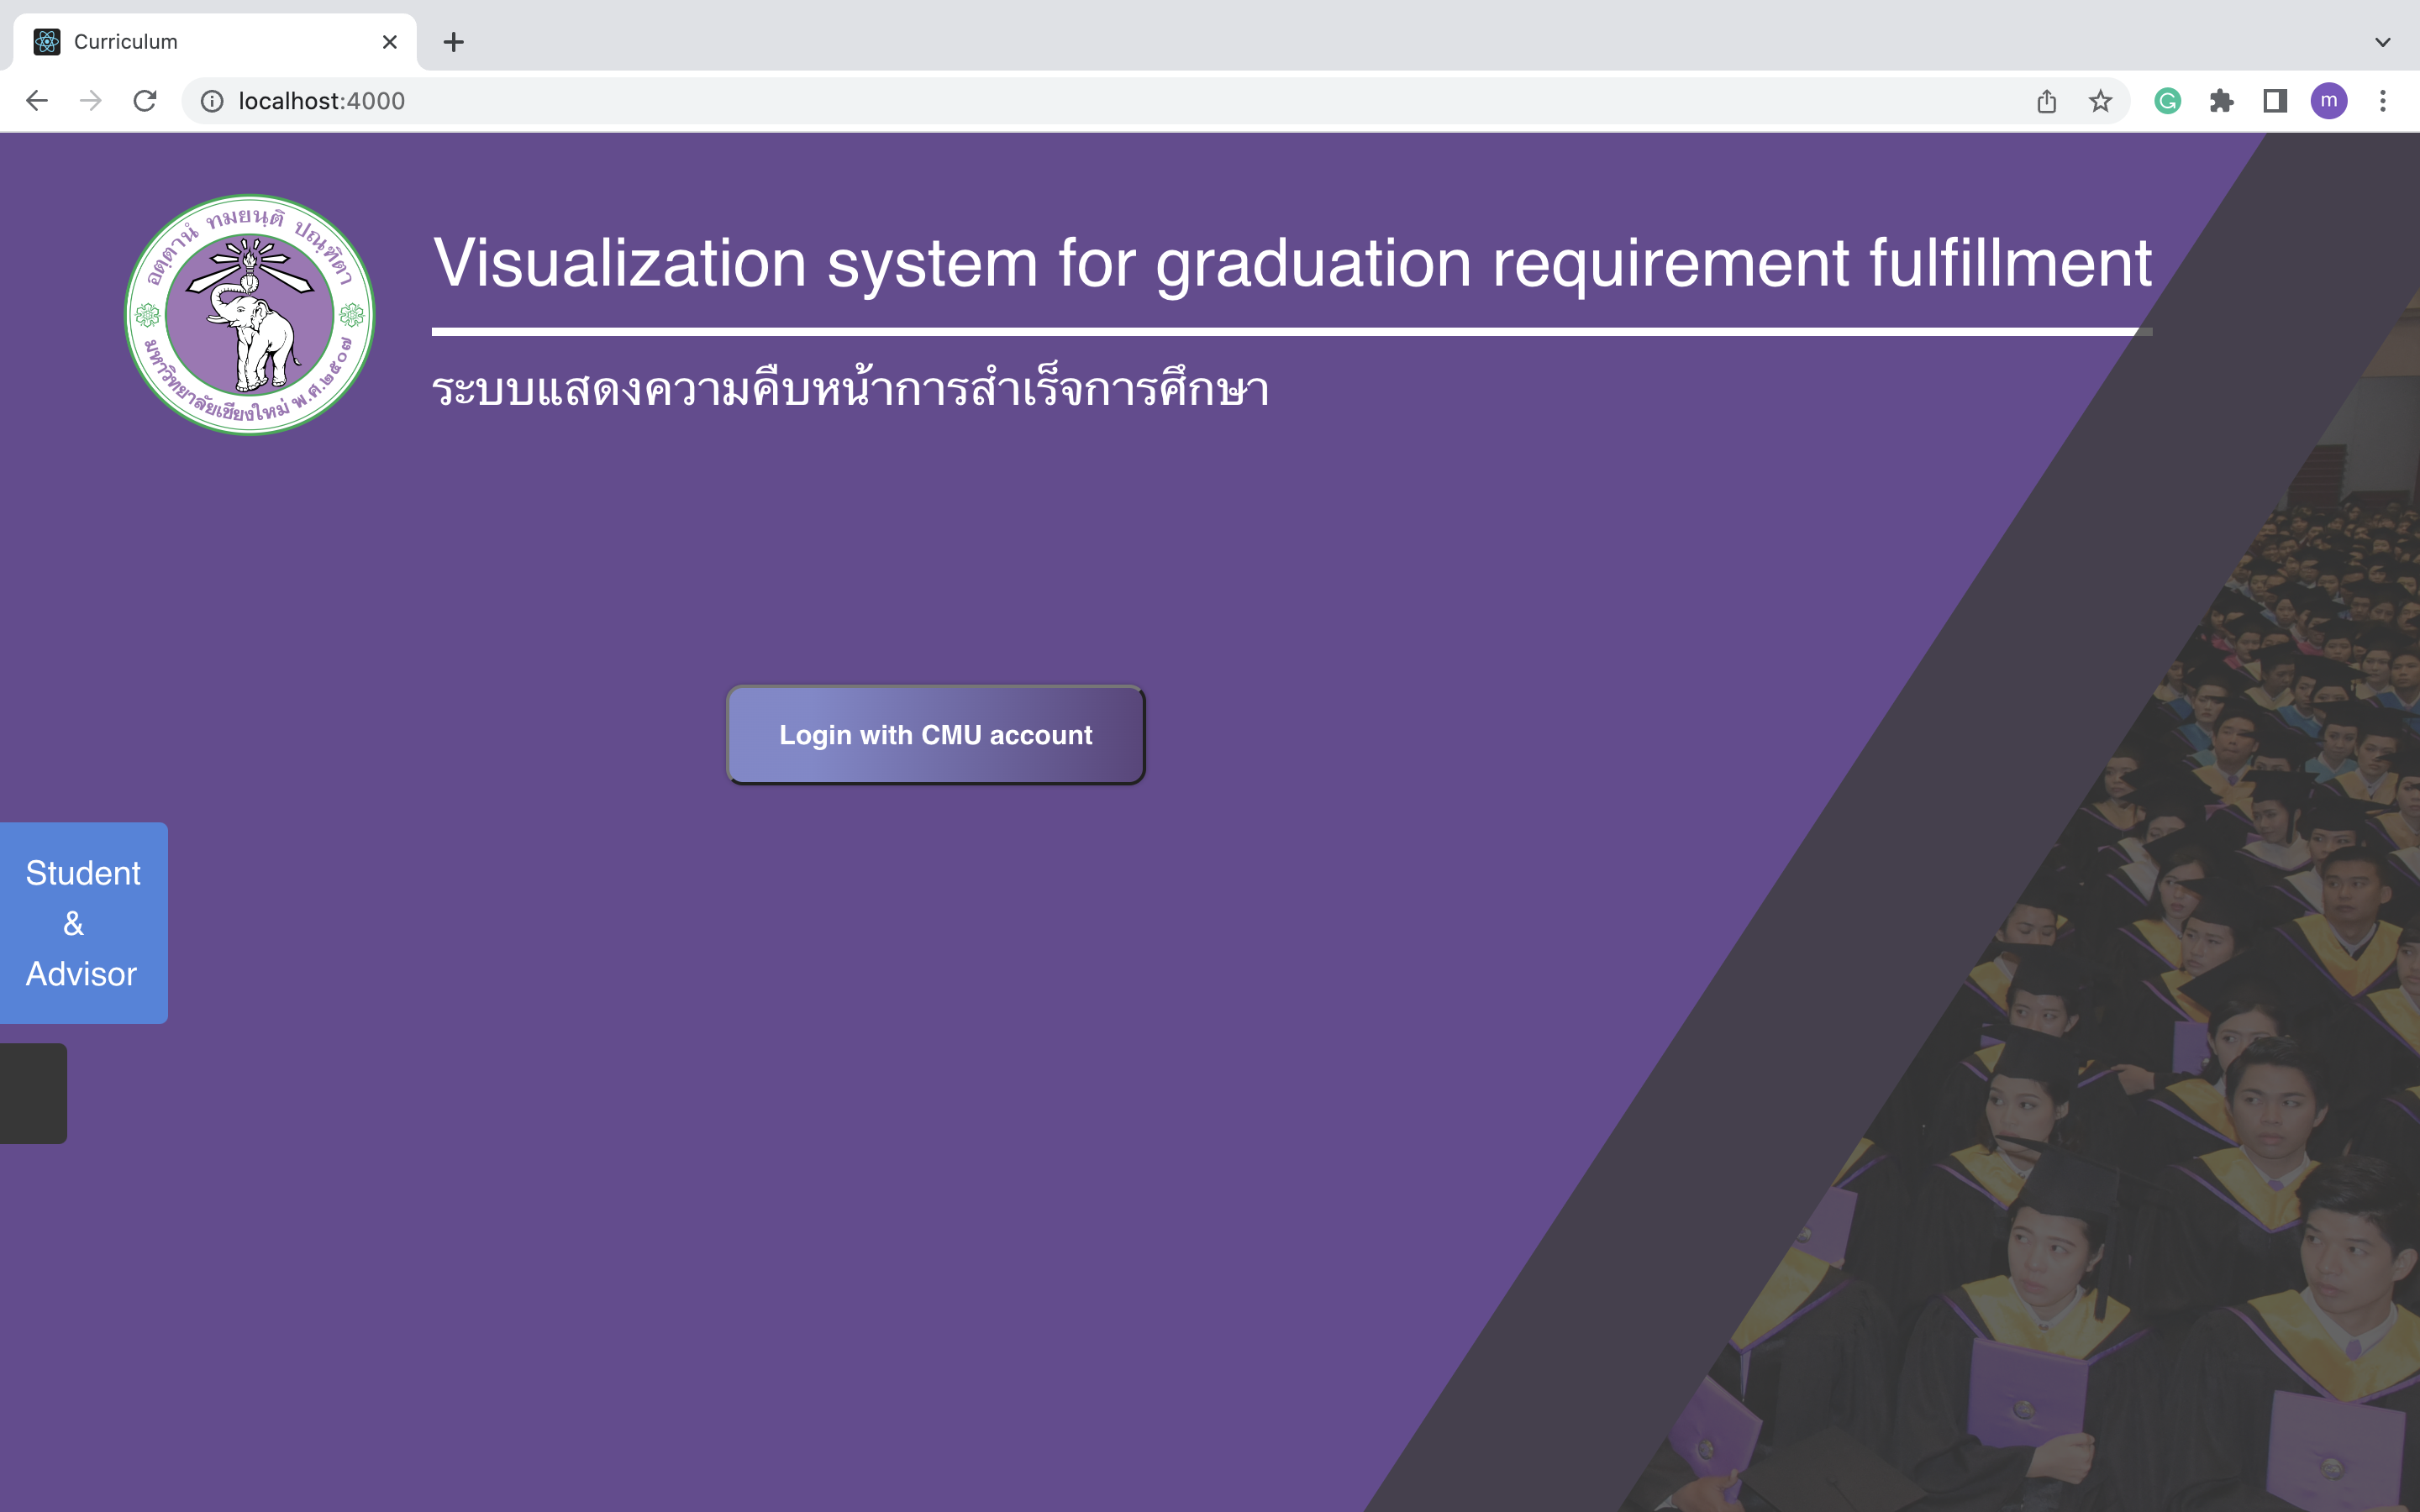
\includegraphics[width=0.8\textwidth]{login.png}}
    \subfigure{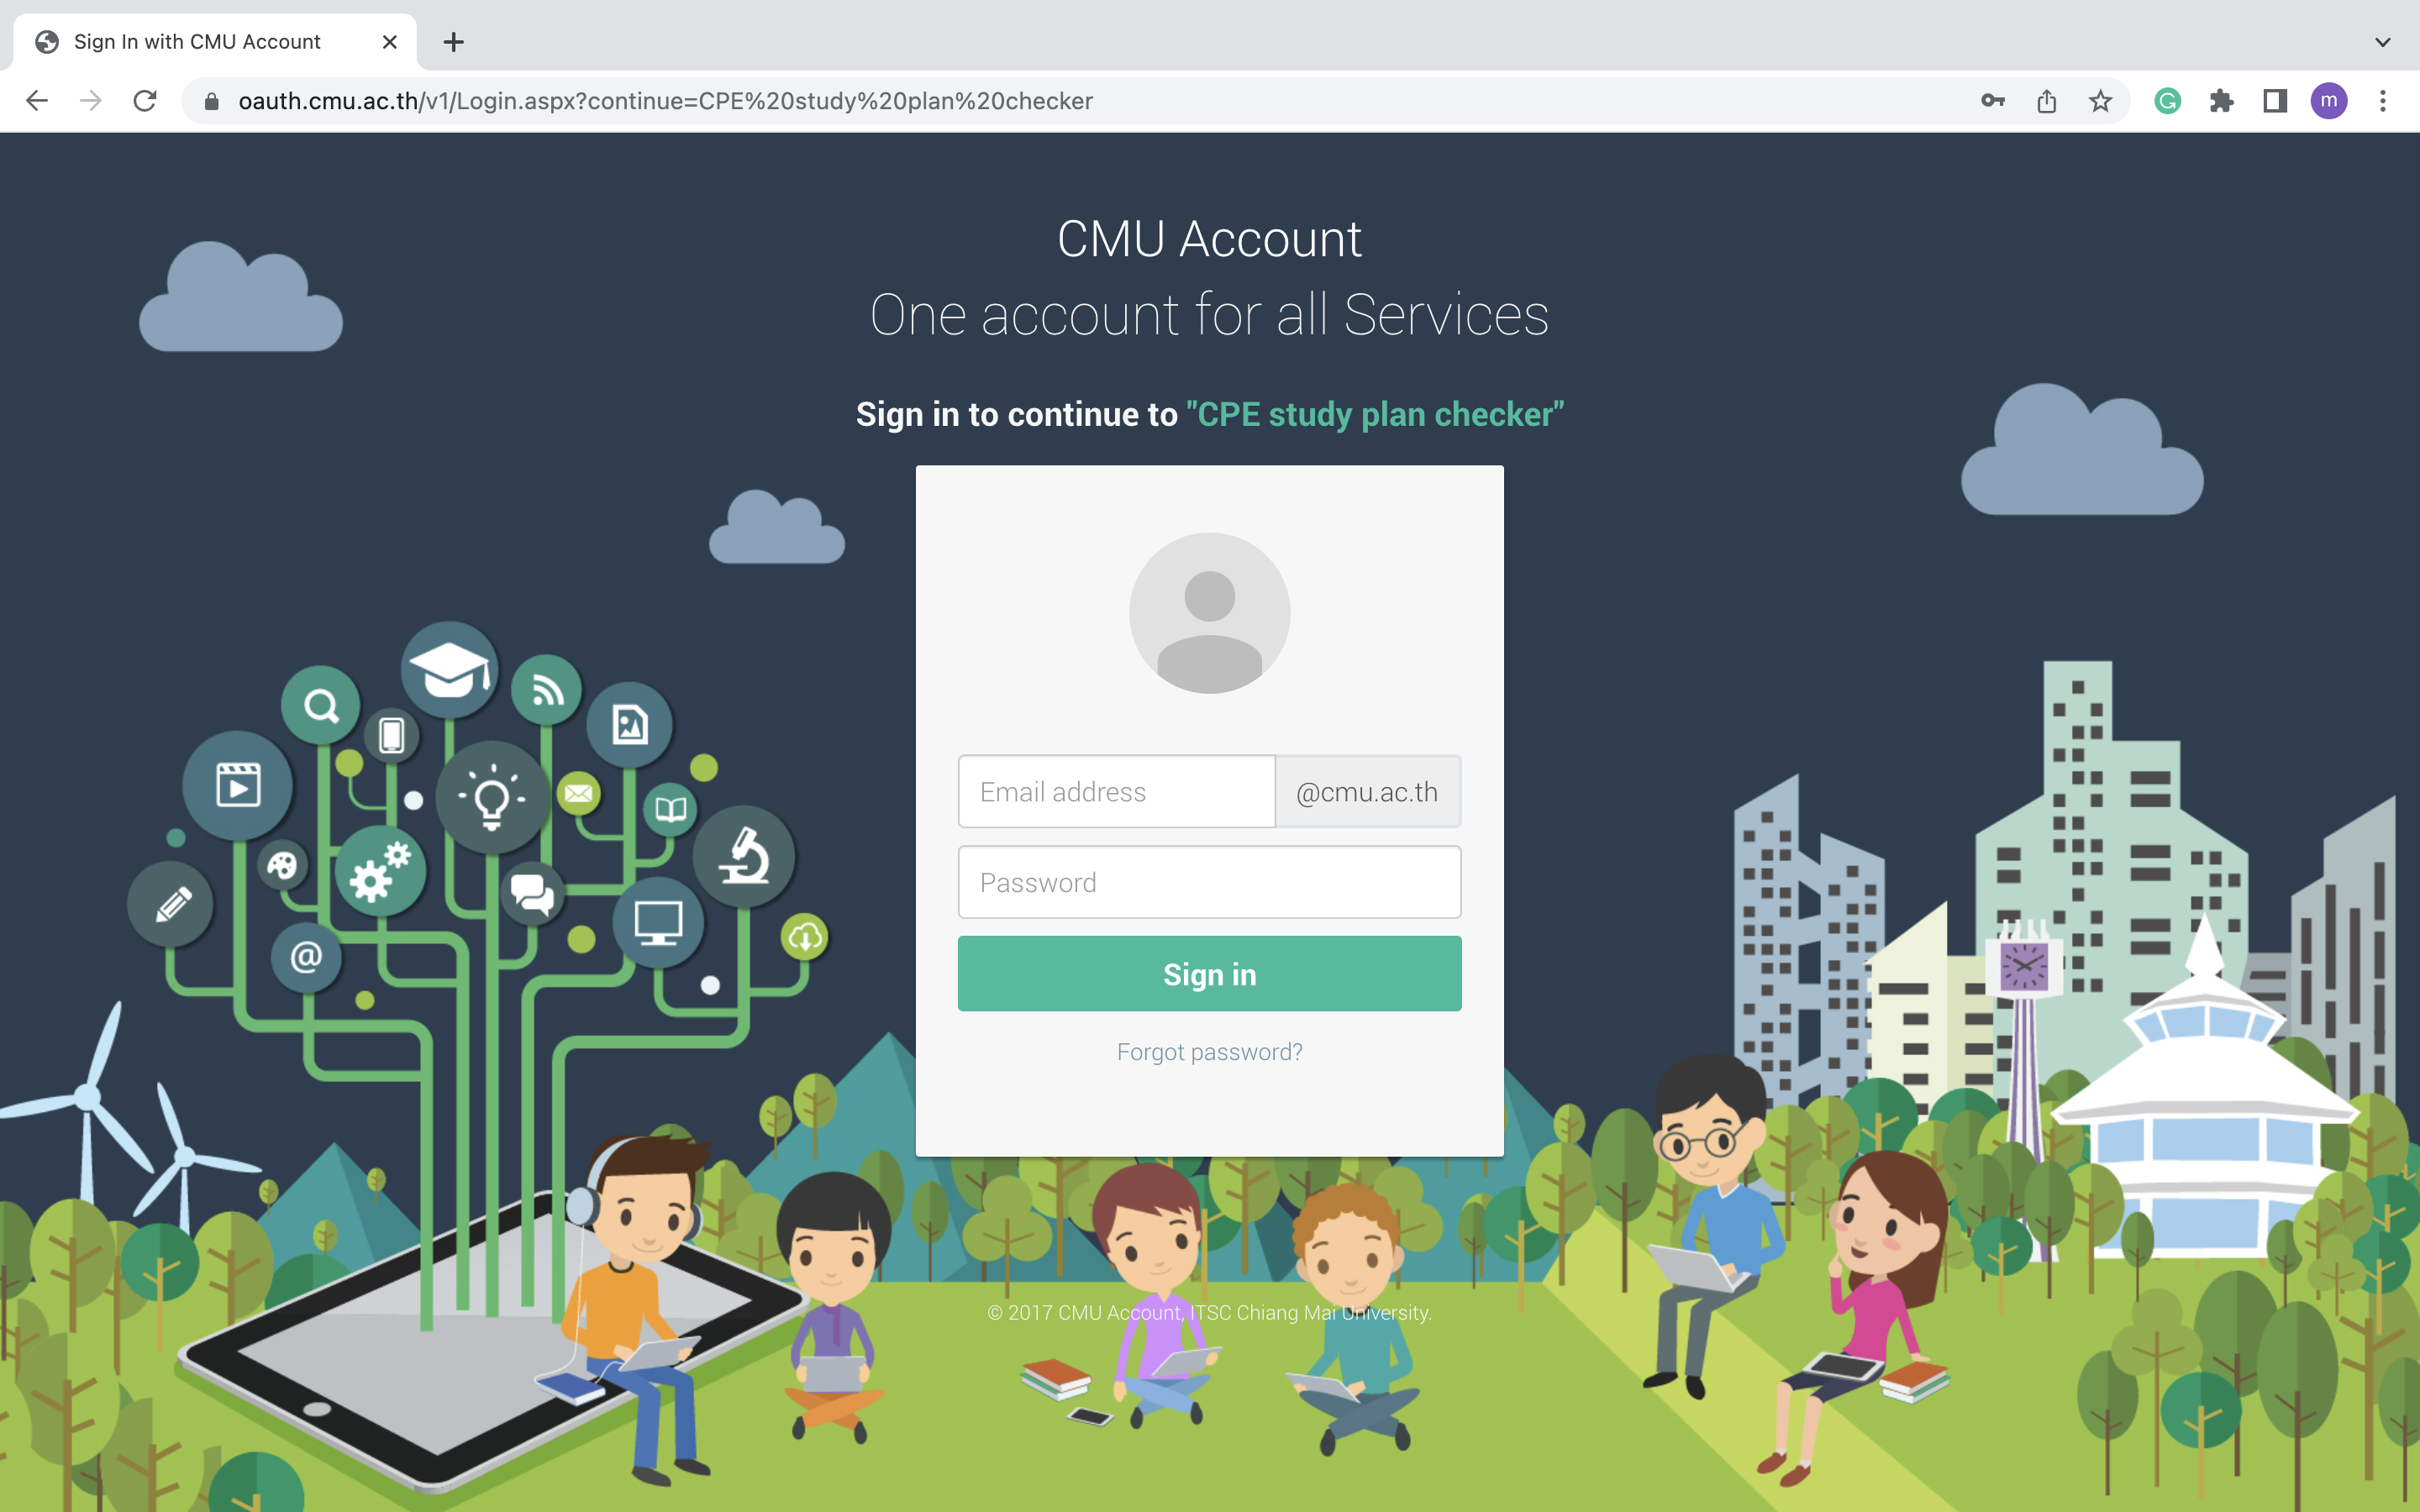
\includegraphics[width=0.8\textwidth]{oauth.png}}
  \end{center}
  \caption{หน้า Advisor Login}
  \label{fig:advisor_login}
\end{figure}

\begin{figure}[H]
  \begin{center}
    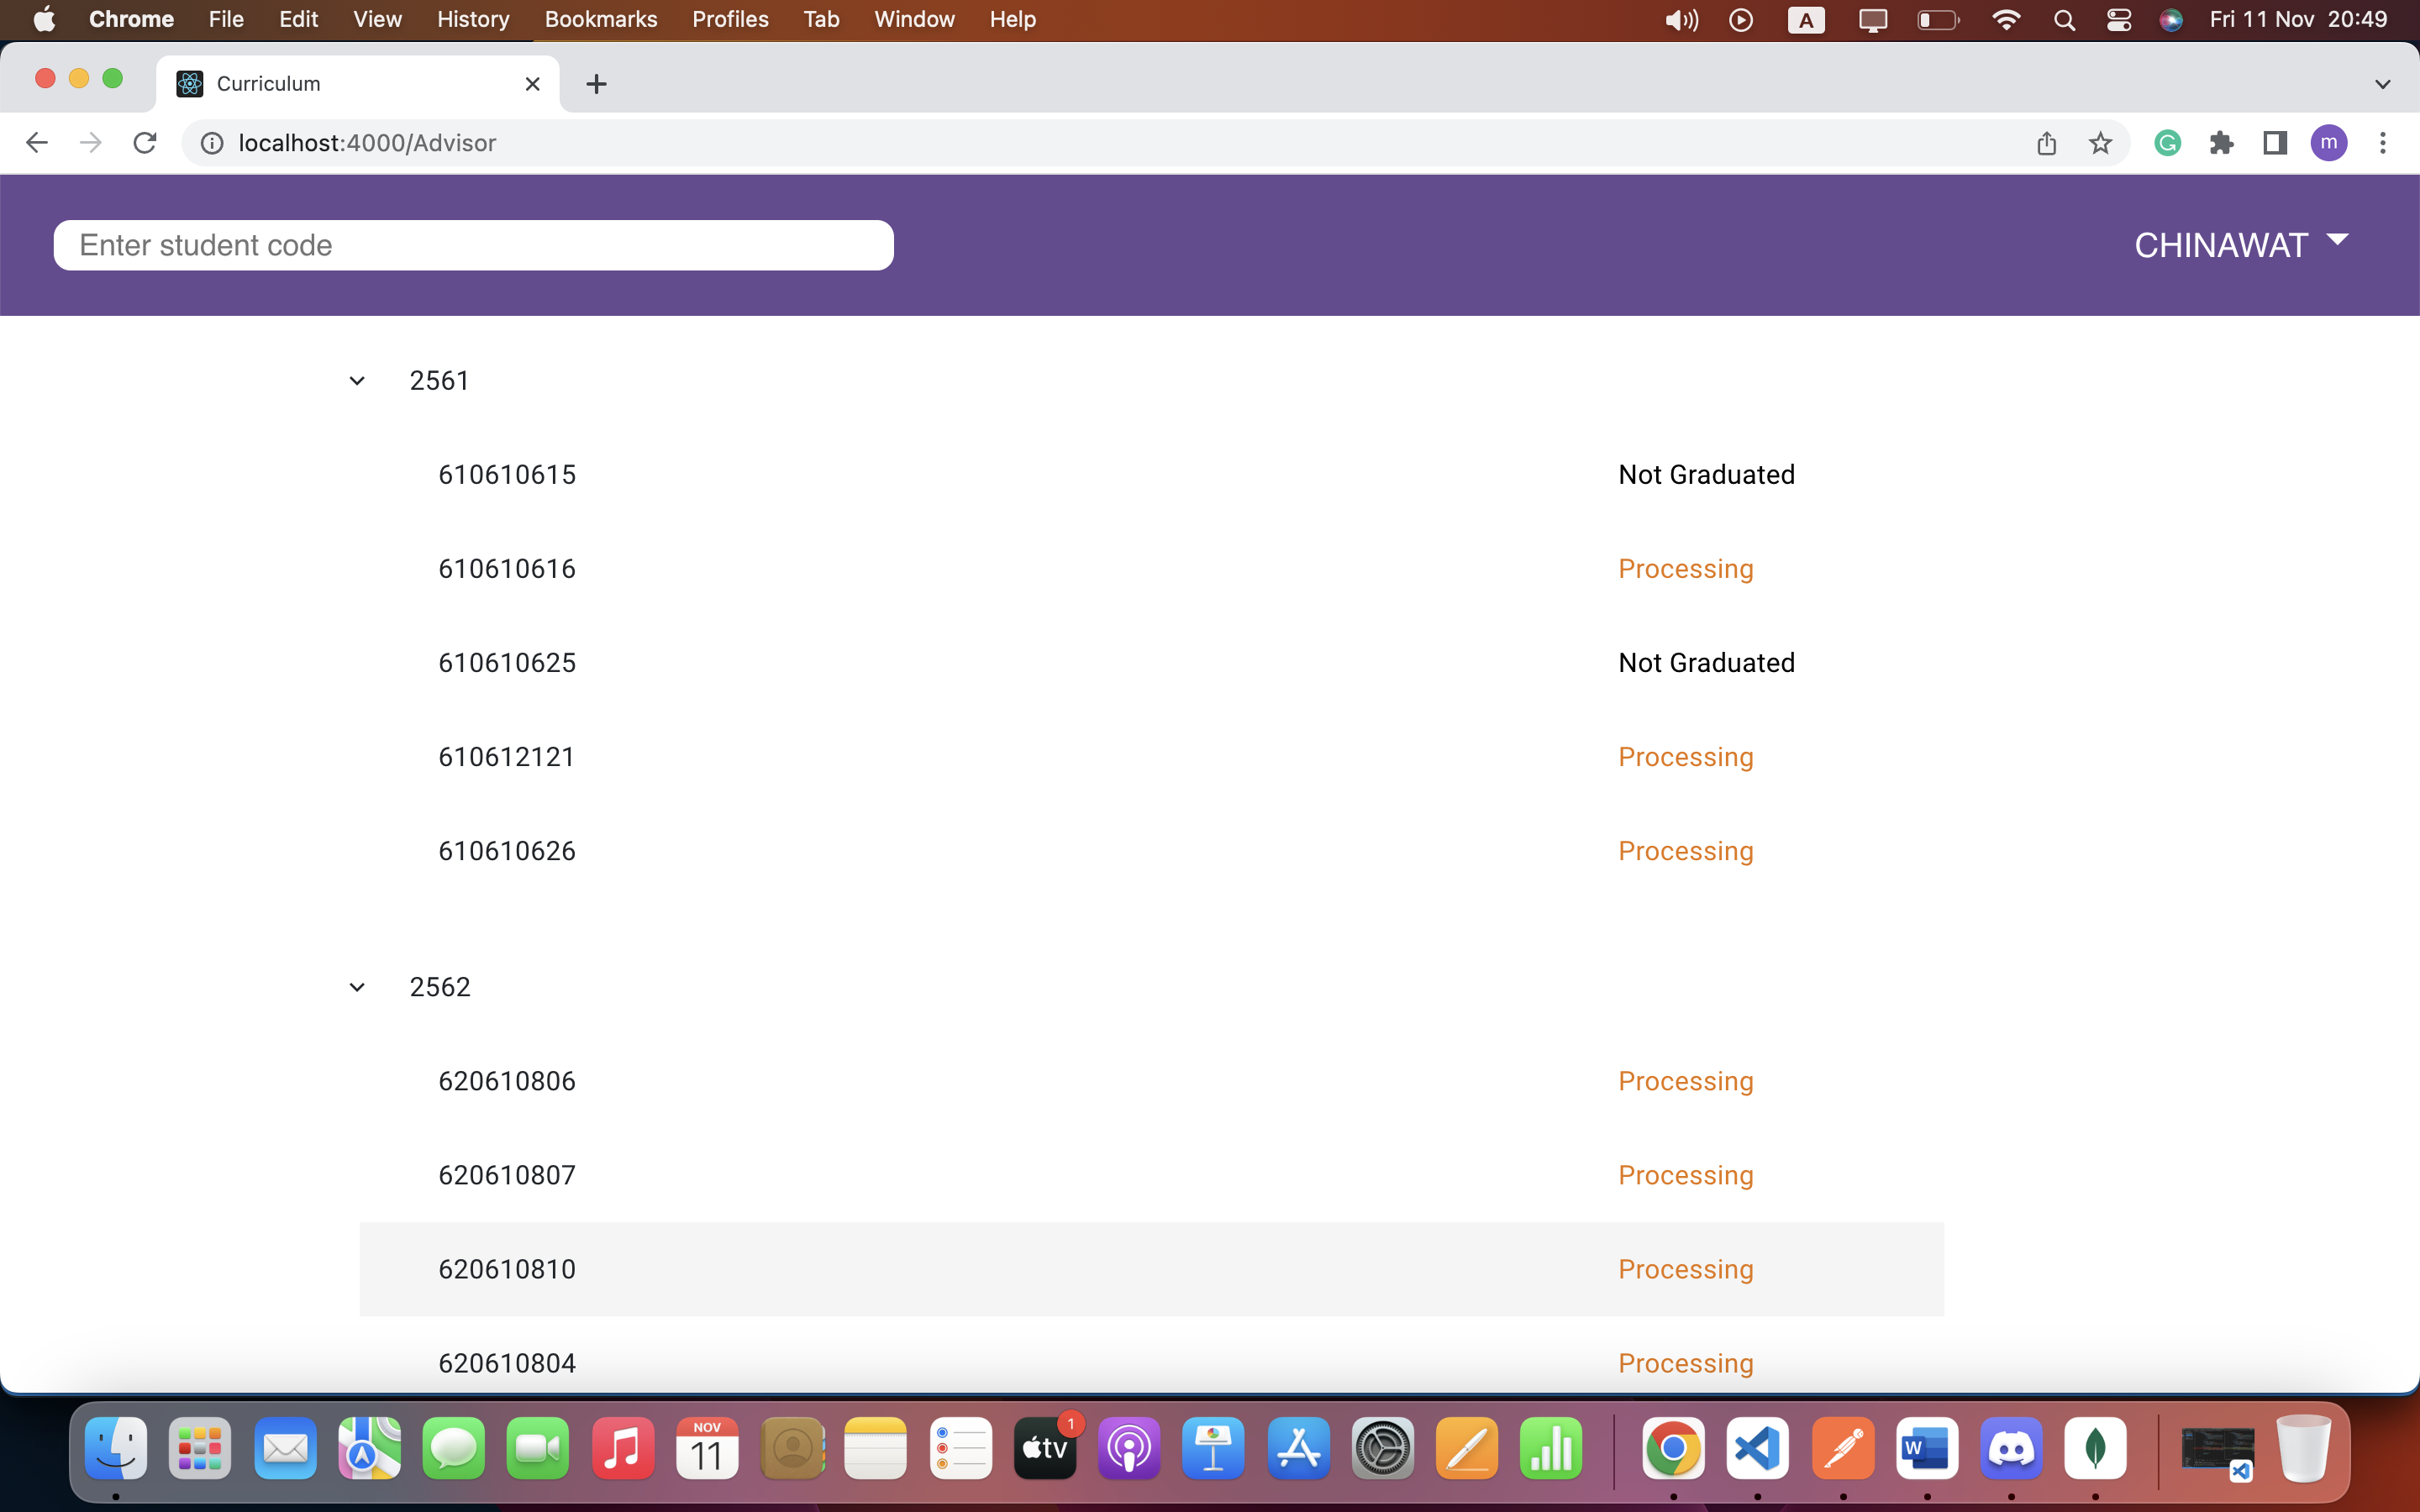
\includegraphics[width=0.8\textwidth]{advisor.png}
    \caption{หน้าเเสดงสถานะนักศึกษา ของอาจารย์ที่ปรึกษา}
    \label{fig:advisor}
  \end{center}
\end{figure}

การใช้งานของอาจารย์ที่ปรึกษา ระบบจะแบ่งกลุ่มของนักศึกษาที่อยู่ในการดูแลตามปีการศึกษาที่นักศึกษาเข้าศึกษา ซึ่ง
อาจารย์ที่ปรึกษาสามารถเข้าไปดูความคืบหน้าของนักศึกษาได้จาก สถานะทางริมขวามือของรหัสนักศึกษา

\subsection{หน้าเว็บสำหรับผู้ดูแลหลักสูตร}

\begin{figure}[H]
  \begin{center}
    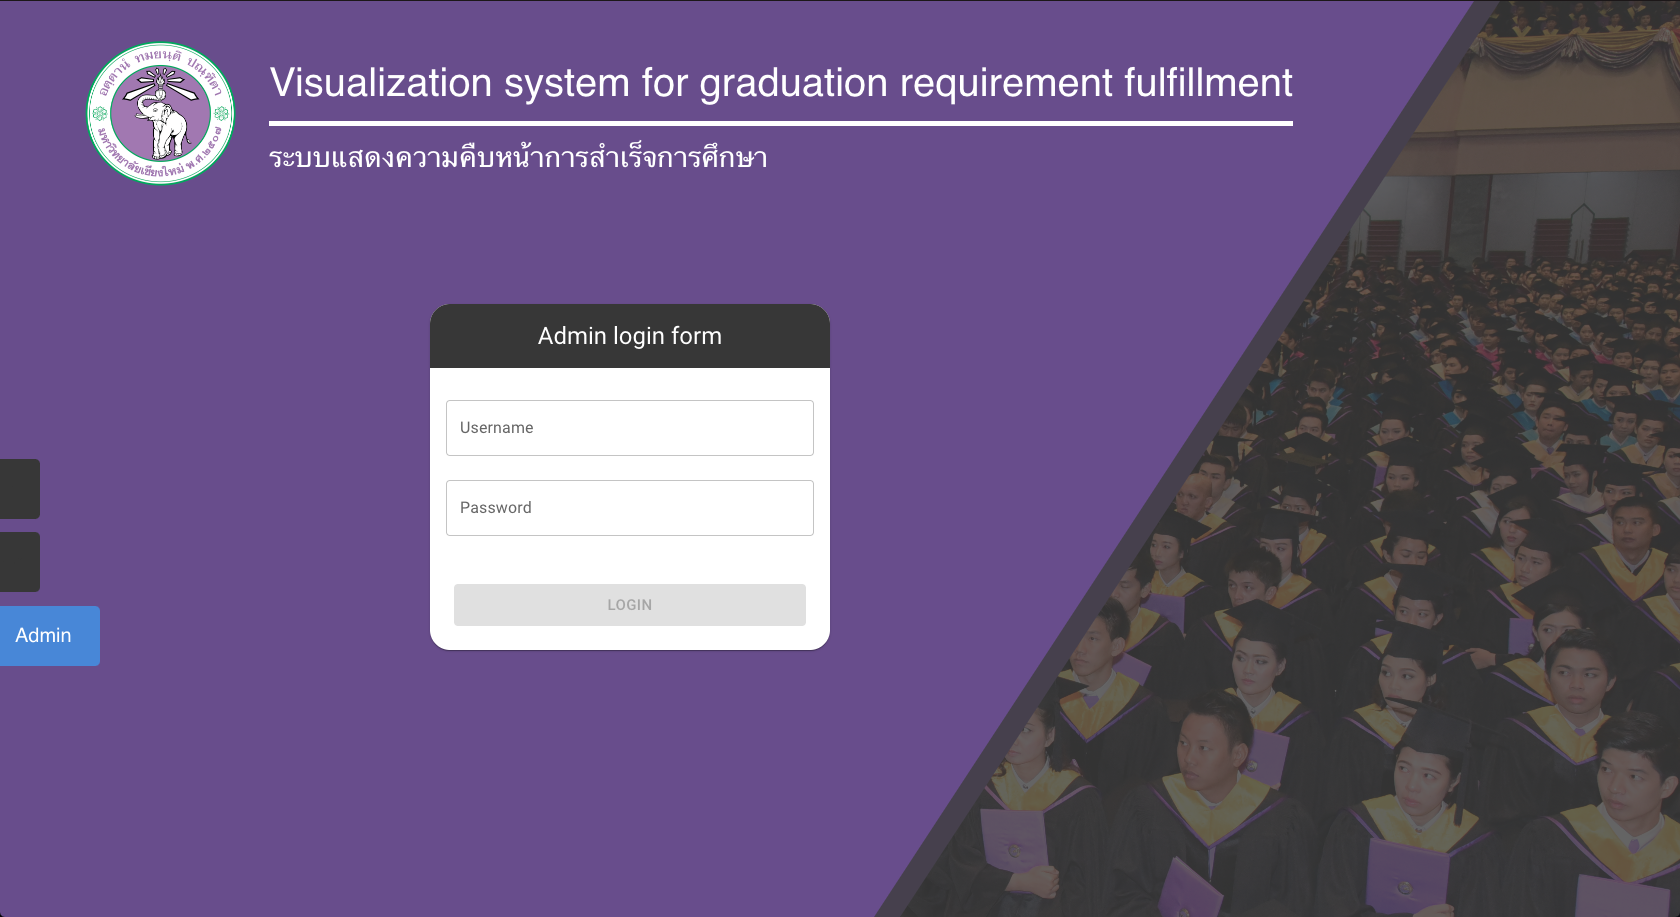
\includegraphics[width=0.8\textwidth]{admin_login.png}
    \caption{หน้า Admin Login}
    \label{fig:admin_login}
  \end{center}
\end{figure}

\begin{figure}[H]
  \begin{center}
    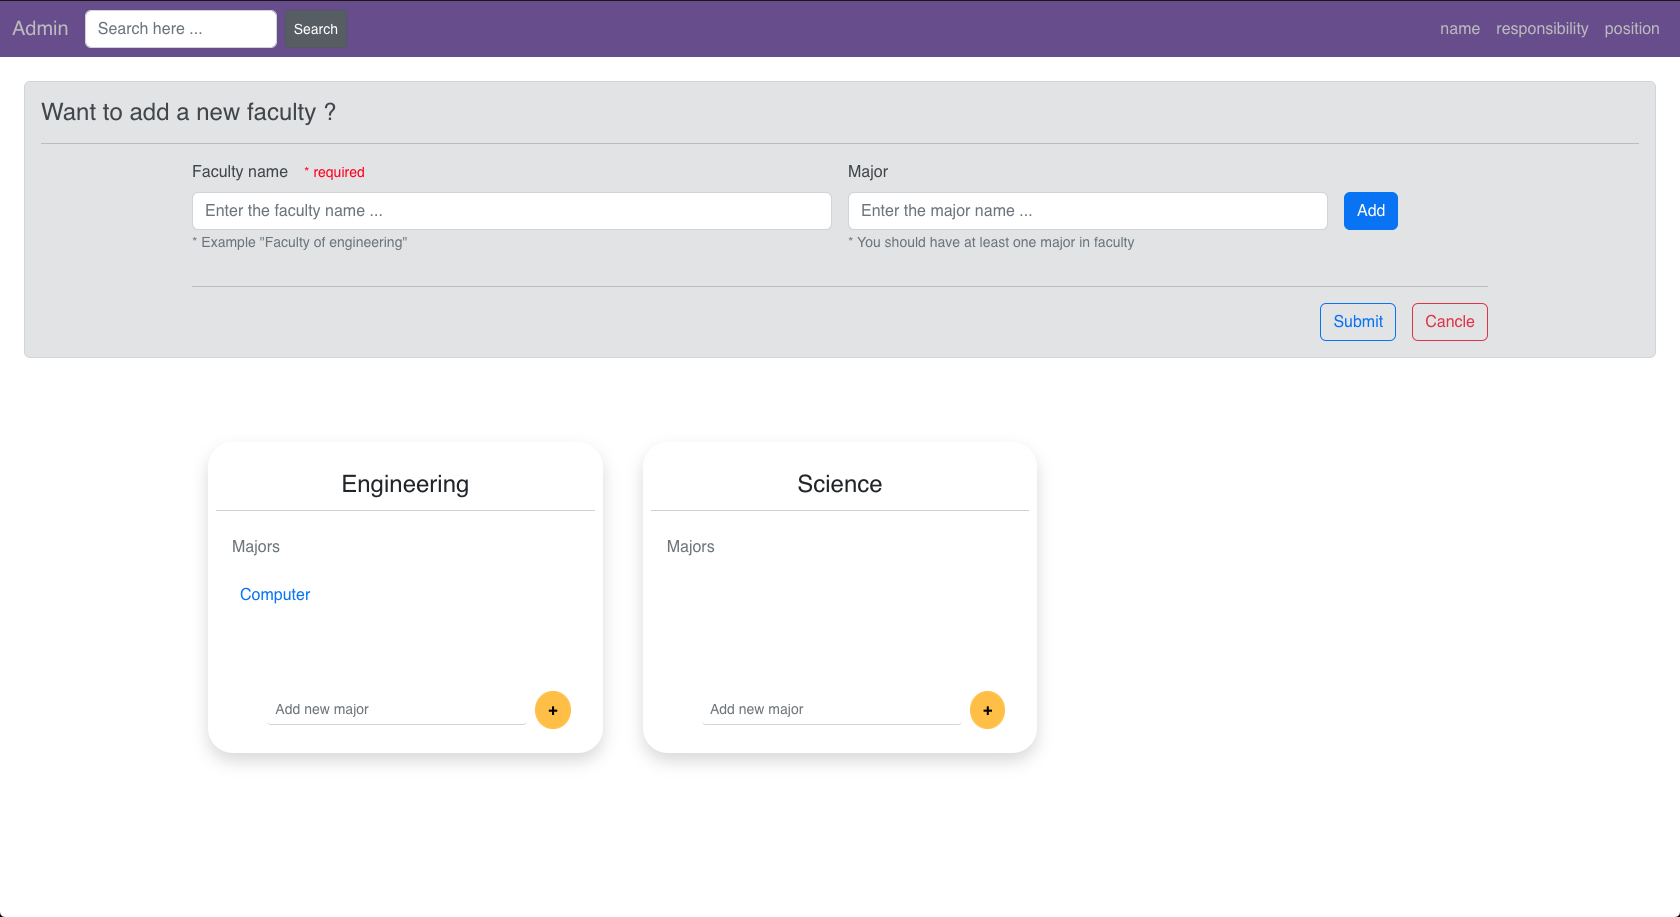
\includegraphics[width=0.8\textwidth]{big_admin.png}
    \caption{หน้าจัดการข้อมูลในระดับ คณะ และสาขา}
    \label{fig:big_admin}
  \end{center}
\end{figure}

\begin{figure}[H]
  \begin{center}
    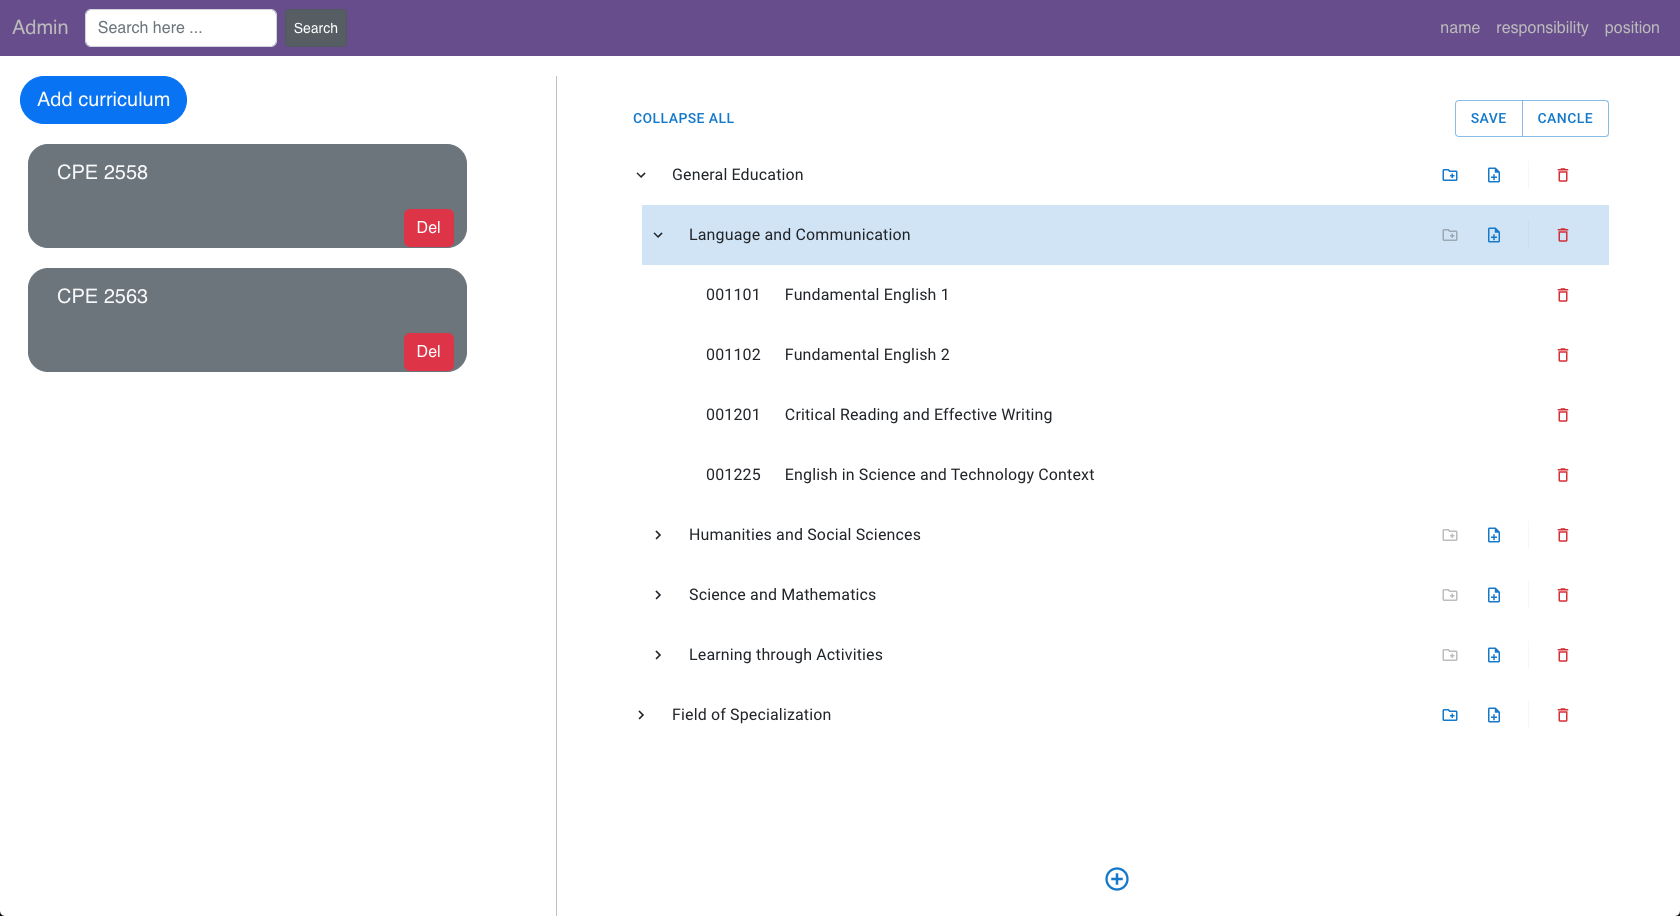
\includegraphics[width=0.8\textwidth]{admin.png}
    \caption{หน้าจัดการข้อมูลในระดับหลักสูตร}
    \label{fig:admin}
  \end{center}
\end{figure}

การใช้งานของผู้ดูแลระบบหรือแอดมิน ในส่วนของแอดมินในขณะนี้จะแบ่งออกเป็น 3 แบบตามความสามารถในการจัดการ
หลักสูตร ได้แก่ 1. แอดมินระดับมหาวิทยาลัย จะสามารถจัดการหลักสูตรได้ทุกหลักสูตรในมหาวิทยาลัย ซึ่งจะสามารถจัดการ(CUD
(create , update and delete))ได้ตั้งแต่ระดับคณะ สาขาวิชา และหลักสูตรในแต่ละปี รวมถึงการแก้ไข เพิ่ม และลบรายวิชาใน
หลักสูตรนั้นๆด้วย 2. แอดมินระดับคณะสามารถจัดการหลักสูตรได้เพียงแค่ในคณะที่ตนเองดูแลอยู่เท่านั้น ซึ่งจะ CUD ได้ตั้งแต่ระดับ
สาขาวิชาและหลักสูตรในแต่ละปี รวมถึงการแก้ไข เพิ่ม และลบรายวิชาในหลักสูตรนั้นๆด้วย 3. แอดมินระดับภาควิชาสามารถจัดการ
หลักสูตรได้ภายในภาควิชาที่ตนเองดูแลเท่านั้น ซึ่งจะ CUD ได้ในระดับหลักสูตรในแต่ละปี รวมถึงการแก้ไข เพิ่ม และลบรายวิชาใน
หลักสูตรนั้นๆด้วย

\subsection{สรุปข้อมูลการศึกษาหลักสูตร}

\begin{center}
  จากการศีกษาหลักสูตรระดับปริญญาตรีทุกสาขาวิชาของทุกคณะในมหาวิทยาลัยเชียงใหม่ จํานวน 185 หลักสูตร ซึ่งได้ทําการจําแนกความซับซ้อนของแต่ละหลักสูตรเป็นหนึ่งใน 4 ระดับ ดังต่อไปนี้
\end{center}

\begin{figure}[H]
  \begin{center}
    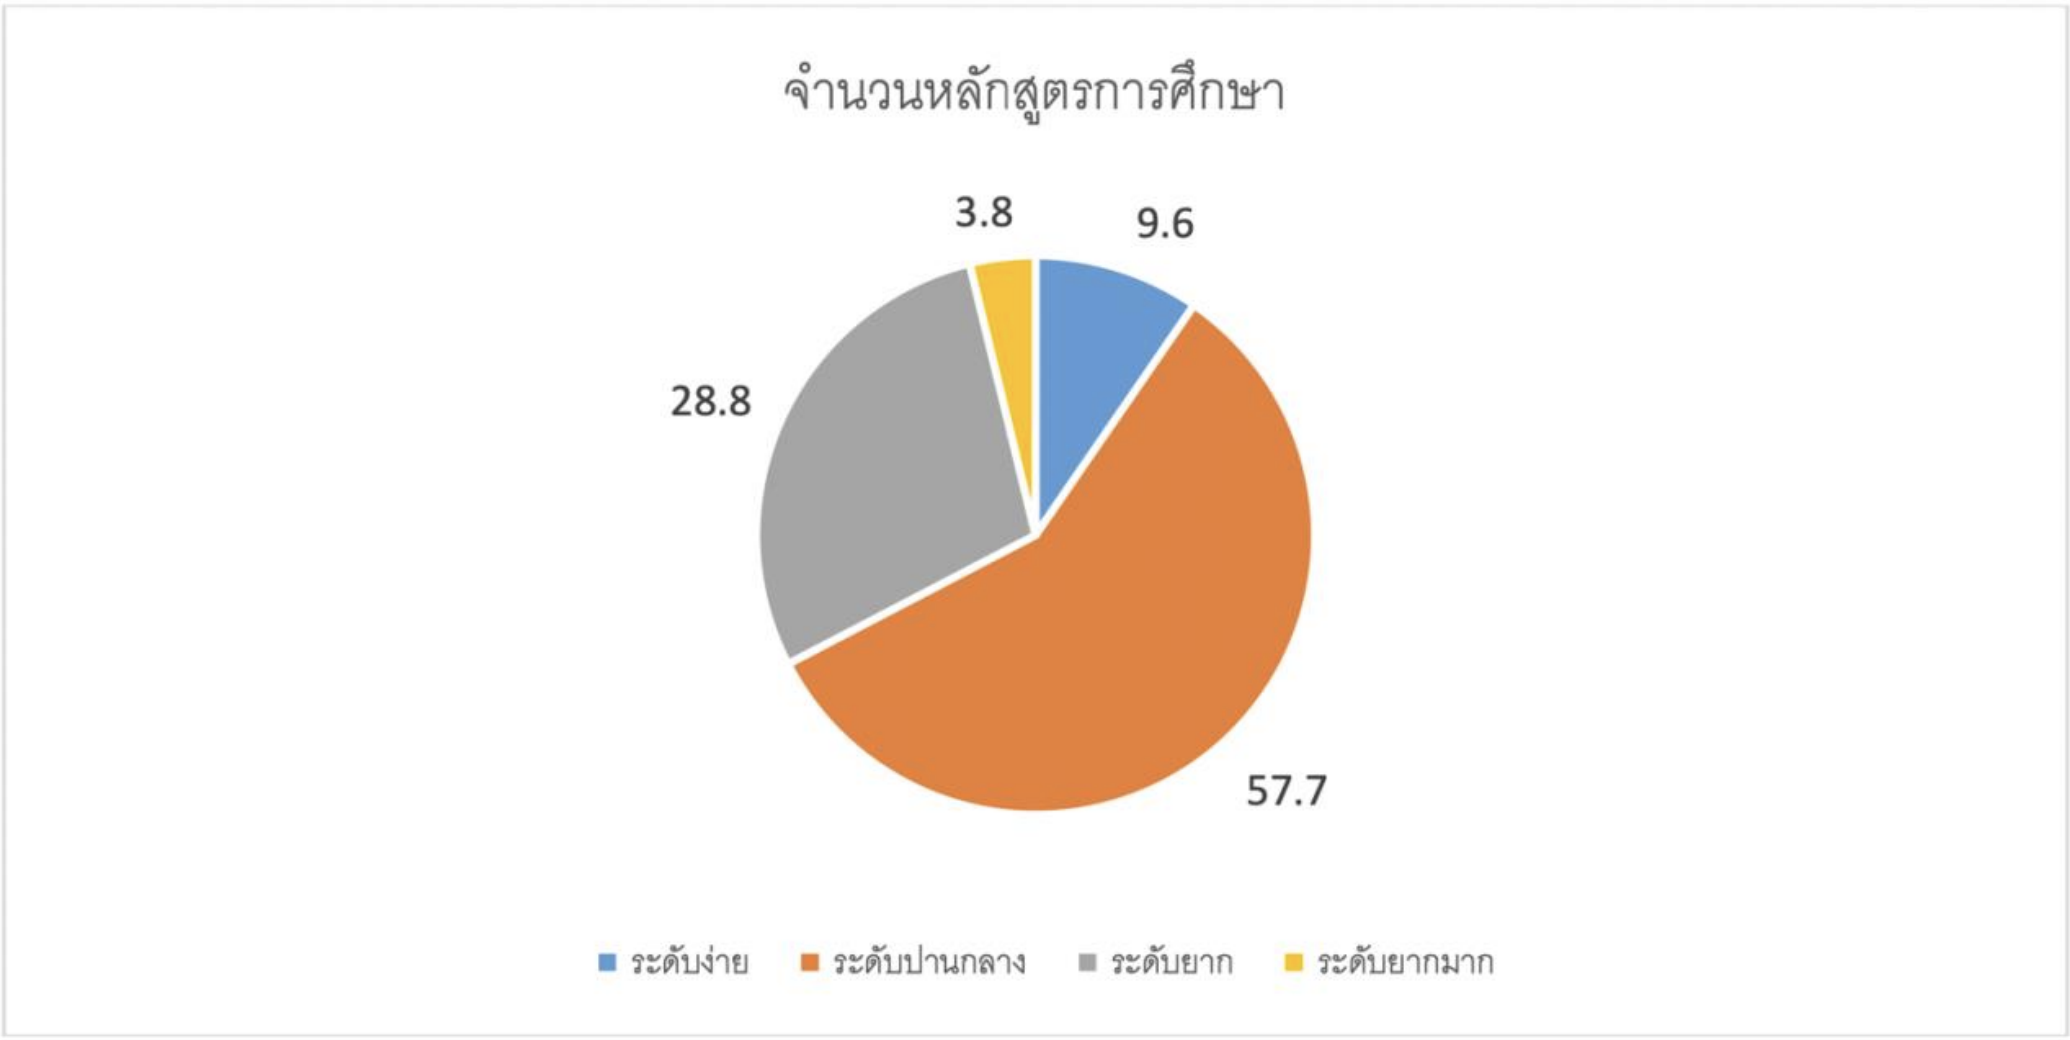
\includegraphics[width=0.8\textwidth]{chart.png}
    \caption{สรุปภาพการศึกษาหลักสูตร}
    \label{fig:chart}
  \end{center}
\end{figure}

\begin{center}
  \begin{minipage}[c]{0.5\linewidth}
     \begin{itemize}
       \item ระดับง่าย 9.6 \%
       \item ระดับปานกลาง 57.7 \%
       \item ระดับยาก 28.8 \%
       \item ระดับยากมาก 3.8 \%
     \end{itemize}
  \end{minipage}
\end{center}

เห็นได้ว่าในหลักสูตรที่พบเห็นได้บ่อยนั้นจะถูกจัดอยู่ในหลักสูตรระดับปานกลาง ดังนั้นในช่วงแรกของการ พัฒนา ผู้พัฒนาจะเริ่มจาก
หลักสูตรระดับปานกลางก่อน และหลักสูตรในระดับยากมากมีทั้งหมด 7 หลักสูตรมีค่าเปอร์เซ็นต์อยู่ที่ 3.8 \% ซึ่งจะมีเพียงบาง
สาขาวิชาเท่านั้น ดังนั้นหลักสูตรที่ถูกจัดอยู่ในระดับ ยากมากทั้งหมดทางผู้พัฒนาจึงขอละเว้นไว้จากขอบเขตของโครงงานนี้


\subsection{การออกแบบโครงสร้างพื้นฐานของข้อมูล}

จากการศึกษาหลักสูตรระดับปริญญาตรีทุกสาขาวิชาของทุกคณะในมหาวิทยาลัยเชียงใหม่ ทําให้เข้าใจโครงสร้าง
เเละรูปเเบบต่างๆของหลักสูตรจึงสามารถสรุป General data model ขึ้นมาได้ ที่จะถูกนําไปใช้สร้าง database ต่อไป

\begin{figure}[H]
  \begin{center}
    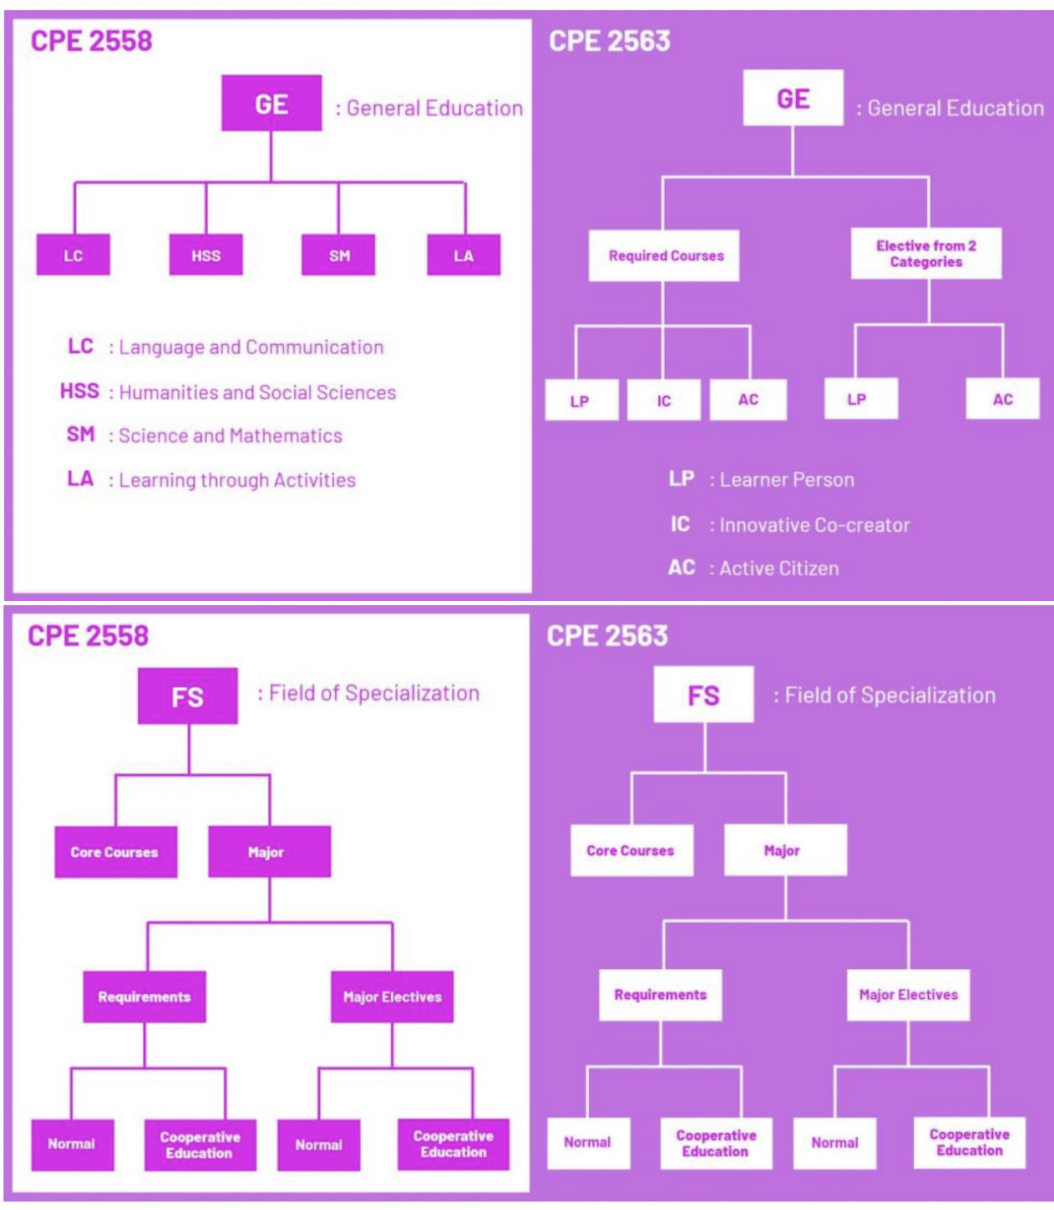
\includegraphics[width=0.8\textwidth]{dModel.png}
    \caption{ตัวอย่าง Data model ของหลักสูตรวิศวกรรมคอมพิวเตอร์}
    \label{fig:dModel}
  \end{center}
\end{figure}

จาก Data model จะสังเกตุได้ว่า ทั้ง 2 หลักสูตรจะมี FS ที่เหมือนกันทำให้สามารถทำ Curriculum data sharing ได้ซึ่ง
ยังมีหลักสูตรอีกจำนวนมาก ที่สามารถทำ Curriculum data sharing ได้

\begin{figure}[H]
  \begin{center}
    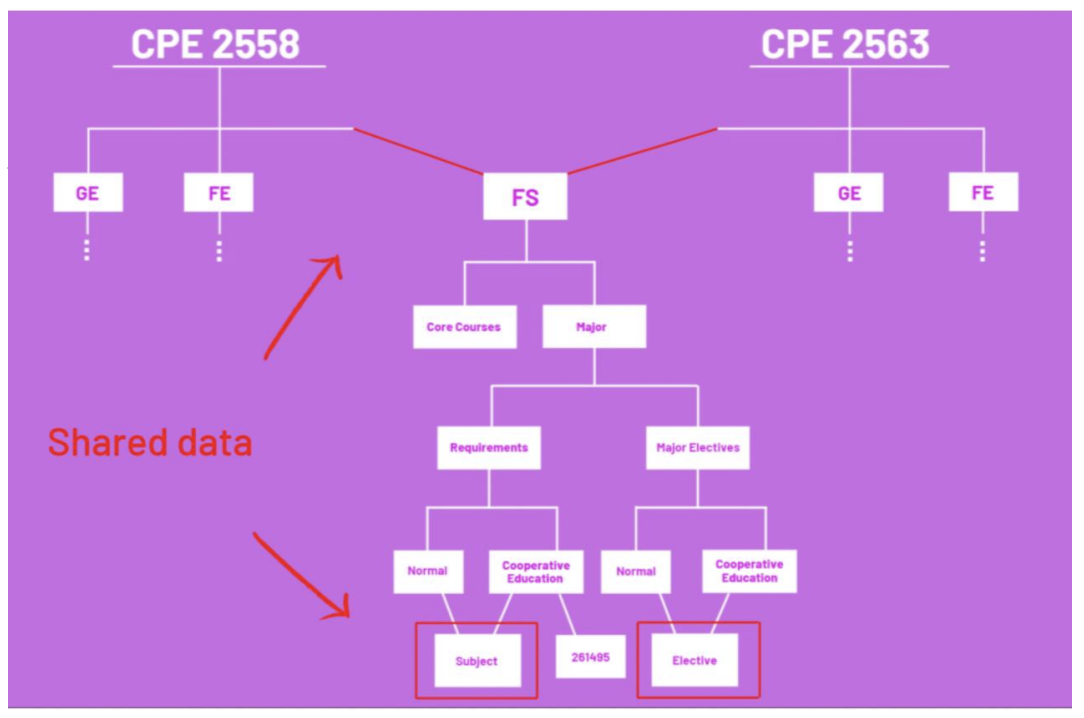
\includegraphics[width=0.8\textwidth]{model.png}
    \caption{Data Sharing}
    \label{fig:model}
  \end{center}
\end{figure}

\begin{enumerate}
  \item Curriculum data sharing ในกรณีนี้เป็นการ share FS ของหลักสูตร 2558 และ 2563
  \item Node data sharing ใน FS ที่ทั้ง 2 หลักสูตรใช้ร่วมกัน มีการ share Subject และ Elective ระหว่าง Normal และ
  Cooperative Education
\end{enumerate}

\section{ขั้นตอนการดำเนินงาน}
\subsection{ศึกษาโครงสร้างหลักสูตร}
จากขอบเขตของโครงงานที่ตั้งเป้าหมายให้เว็ปแอปพลิเคชั่นนั้นสามารถรองรับได้ในทุกหลักสูตรจึงเป็นผลให้ต้องศึกษาโครงสร้างหลักสูตรในแต่ละหลักสูตร 
และหลังจากที่ทําการศึกษาแล้วนั้นพบว่าในปัจจุบันจะมีหลักสูตรที่ใช้กันอย่างมากในมหาวิทยาลัยเชียงใหม่นั่นก็คือหลักสูตรปีการศึกษา 2558 และหลักสูตรปีการศึกษา 2563 (1 หลักสูตรสามารถใช้ได้ 5 ปีการศึกษา) 
แต่ยังคงมีหลักสูตรในบางสาขาวิชาที่มีการปรับปรุงหลักสูตรก่อนครบ 5 ปีการศึกษา จึงเป็นผลให้ต้องศึกษาโครงสร้างของหลักสูตรนั้นอย่างละเอียดอีกครั้งเพื่อตรวจสอบดูว่ามีหลักสูตรใดบ้างที่มีการปรับปรุงหลักสูตรก่อนครบ 5 ปีการศึกษา 
เพราะถ้าหากพบว่าหลักสูตรใดมีการปรับปรุงหลักสูตรก่อนครบ 5 ปีการศึกษา ทางผู้พัฒนาจะนับเป็นหลักสูตรใหม่ตามปีการศึกษาที่ประกาศใช้หลักสูตรนั้นทันที
\subsection{จำแนกระดับความซับซ้อนของหลักสูตร}
ในระหว่างที่ทำการศึกษาโครงสร้างหลักสูตรแต่ละอันนั้นผู้พัฒนาได้ทำการจำแนกหลักสูตรตามระดับความซับซ้อนของหลักสูตรด้วยเช่นกัน 
โดยทำการจำแนกจากความสามารถในการเลือกแผนการเรียนภายในหลักสูตรนั้นๆซึ่งจะได้ออกมาดังนี้
\begin{enumerate}
  \item หลักสูตรระดับง่าย - คือหลักสูตรที่ไม่สามารถเลือกแผนการเรียนตามความสนใจของนักศึกษาได้ กล่าวอีกนัยนึงคือมีแค่แผนการเรียนเดียวในหลักสูตรนั้นจึงทำให้มีโครงสร้างหลักสูตรที่ไม่ซับซ้อน
	ตัวอย่างเช่น
  \begin{itemize}
    \item หลักสูตรปีการศึกษา 2564 สาขาวิศวกรรมหุ่นยนต์ ที่มีแผนการเรียนแบบปกติ ( Normal ) เพียงอย่างเดียว
    \item หลักสูตรปีการศึกษา 2561 สาขาพยาบาลศาสตร์ ที่มีแผนการเรียนแบบสหกิจศึกษา ( Co-operative ) เพียงอย่างเดียว
  \end{itemize}
  \item หลักสูตรระดับปานกลาง - คือหลักสูตรที่มีแผนการเรียนทั้งแบบปกติและแบบสหกิจศึกษา ทำให้สามารถเลือกเรียนได้มากกว่า 1 รูปแบบ ดังนั้นโครงสร้างหลักสูตรจึงมีความซับซ้อนมากขึ้น ซึ่งหลักสูตรในระดับปานกลางนี้จะพบได้ในหลายคณะ
  ตัวอย่างเช่น
  \begin{itemize}
    \item หลักสูตรปีการศึกษา 2558 และ 2563 สาขาวิศวกรรมคอมพิวเตอร์
  \end{itemize}
  \item หลักสูตรระดับยาก - คือหลักสูตรที่มีแผนการเรียนทั้งแบบปกติ แบบสหกิจศึกษา และยังสามารถเลือกความถนัดในหลักสูตรของตนเองได้อย่างอิสระ ทำให้โครงสร้างหลักสูตรนั้นมีความซับซ้อนมาก และต้องทำการเทียบกระบวนวิชาที่สอดคล้องกันในแต่ละหมวดของความถนัด
  ตัวอย่างเช่น
  \begin{itemize}
    \item หลักสูตรปีการศึกษา 2558 และ 2563 สาขาวิศวกรรมไฟฟ้า ที่สามารถเลือกแผนการเรียนได้ 2 รูปแบบและสามารถเลือกหมวดความถนัดภายในสาขาวิชาตามที่สนใจได้อีก 2 หมวดได้แก่ ไฟฟ้ากำลัง และไฟฟ้าสื่อสาร
  \end{itemize}
  \item หลักสูตรระดับยากมาก - คือหลักสูตรที่มีแผนการเรียนทั้งแบบปกติ แบบสหกิจศึกษา เลือกหมวดความถนัด และในหมวดความถนัดแต่ละอันก็ยังคงเลือกได้อีกว่าจะเรียนหมวดความถนัดย่อยใดต่อไป ทำให้โครงสร้างหลักสูตรนั้นมีความซับซ้อนอยู่ในระดับยากที่สุด
  ตัวอย่างเช่น
  \begin{itemize}
    \item หลักสูตรปีการศึกษา 2558 และ 2563 คณะเภสัชศาสตร์
    \item หลักสูตรปีการศึกษา 2558 และ 2563 คณะเกษตรศาสตร์ สาชาวิชาเกษตรศาสตร์
  \end{itemize}
\end{enumerate}

\subsection{ออกแบบระบบ}
\begin{itemize}
  \item ออกแบบ UX/UI ของระบบด้วยโปรแกรม Adobe XD แต่เนื่องจากเกิดปัญหาในการใช้ plug-in ของโปรแกรม Adobe XD ผู้พัฒนาจึงเปลี่ยนไปใช้โปรแกรม 
  Figma แทน
  \item ออกเเบบ Data Model เเละ Database
\end{itemize}

\subsection{พัฒนาระบบ}

Frontend
\begin{itemize}
  \item พัฒนาหน้าเว็บไซค์ตามที่ได้ออกแบบ UX/UI เอาไว้ โดยนำข้อมูลจำลองที่ออกแบบมาใช้เป็นตัวอย่างในการพัฒนาขั้นต้น
  \item เชื่อมต่อ Apollo client ในฝั่ง front-end
  \item พัฒนาและเรียกใช้งาน query ต่างๆเพื่อดึงข้อมูลจริงจากฝั่ง back-end
\end{itemize}
Backend
\begin{itemize}
  \item คํานวณ เทียบหลักสูตรการศึกษาที่มีในระบบ กับข้อมูลการลงทะเบียนของนักศึกษา เพื่อเช็คสถานะต่างๆ 
  ของนักศึกษา อาทิ (เกรด, เกรดเฉลี่ย, รายวิชาที่ลง, หมวดต่างๆที่ต้องลงตามหลักสูตร ) เเละส่งออกมาเป็น ข้อมูลที่มีลําดับขั้น(Tree) ก่อนส่งต่อให้ Frontend
  \item พัฒนา Backend server ประมวลผลข้อมูลก่อนสร้างก้อนข้อมูล ด้วย Graphql 
  \item พัฒนา Graphql schema และ Graphql resolvers เพื่อตอบสนองการดึงข้อมูลผ่าน Frontend ด้วย Apollo client
  \item พัฒนา Apollo server ในฝั่ง back-end
  \item พัฒนาเเละ จัดการ ฐานข้อมูล MongoDB ผ่าน Mongoose
\end{itemize}

\subsection{ทดลองใช้งาน}
\begin{itemize}
  \item ผู้พัฒนาได้ทดลองล็อกอินผ่าน CMU Account เพื่อเข้าใช้งานระบบและพัฒนาระบบอยู่เสมอ
  \item ให้นักศึกษา CPE ทดลองเข้าสู่ระบบโดยล็อกอินผ่านคอมพิวเตอร์ของผู้พัฒนา (เวอร์ชันก่อน deploy และ test)
  \item Deploy ระบบให้สามารถเข้าใช้งานผ่านลิงก์ พร้อมทั้งแนบแบบสอบถามเพื่อเก็บผลประเมินหลังการใช้งานระบบแสดงความคืบหน้าการสำเร็จการศึกษา
\end{itemize}


\chapter{\ifproject%
\ifenglish Experimentation and Results\else การทดลองและผลลัพธ์\fi
\else%
\ifenglish System Evaluation\else การประเมินระบบ\fi
\fi}

ในบทนี้จะทดสอบเกี่ยวกับการทํางานในฟังก์ชันหลักๆ ของแอปพลิเคชัน โดยเนื้อหาจะกล่าวถึงคือโมดูลการทํางานต่างๆ ของระบบ

\subsection{การทดสอบระบบ API ของ backend}
เนื่องจาก API หลักๆในระบบ จะถูกส่งด้วย GraphQL เราจึงได้มีการทดสอบ ทุก Resolvers ในระบบ เเละจากการทดสอบไม่พบข้อผิดพลาดใดๆ
\begin{center}
    \begin{minipage}[c]{0.5\linewidth}
       \begin{itemize}
         \item ยกตัวอย่างการดึงข้อมูลหมวดต่างๆ ที่เก็บรายวิชา
       \end{itemize}
    \end{minipage}
  \end{center}

  \begin{figure}[H]
    \begin{center}
      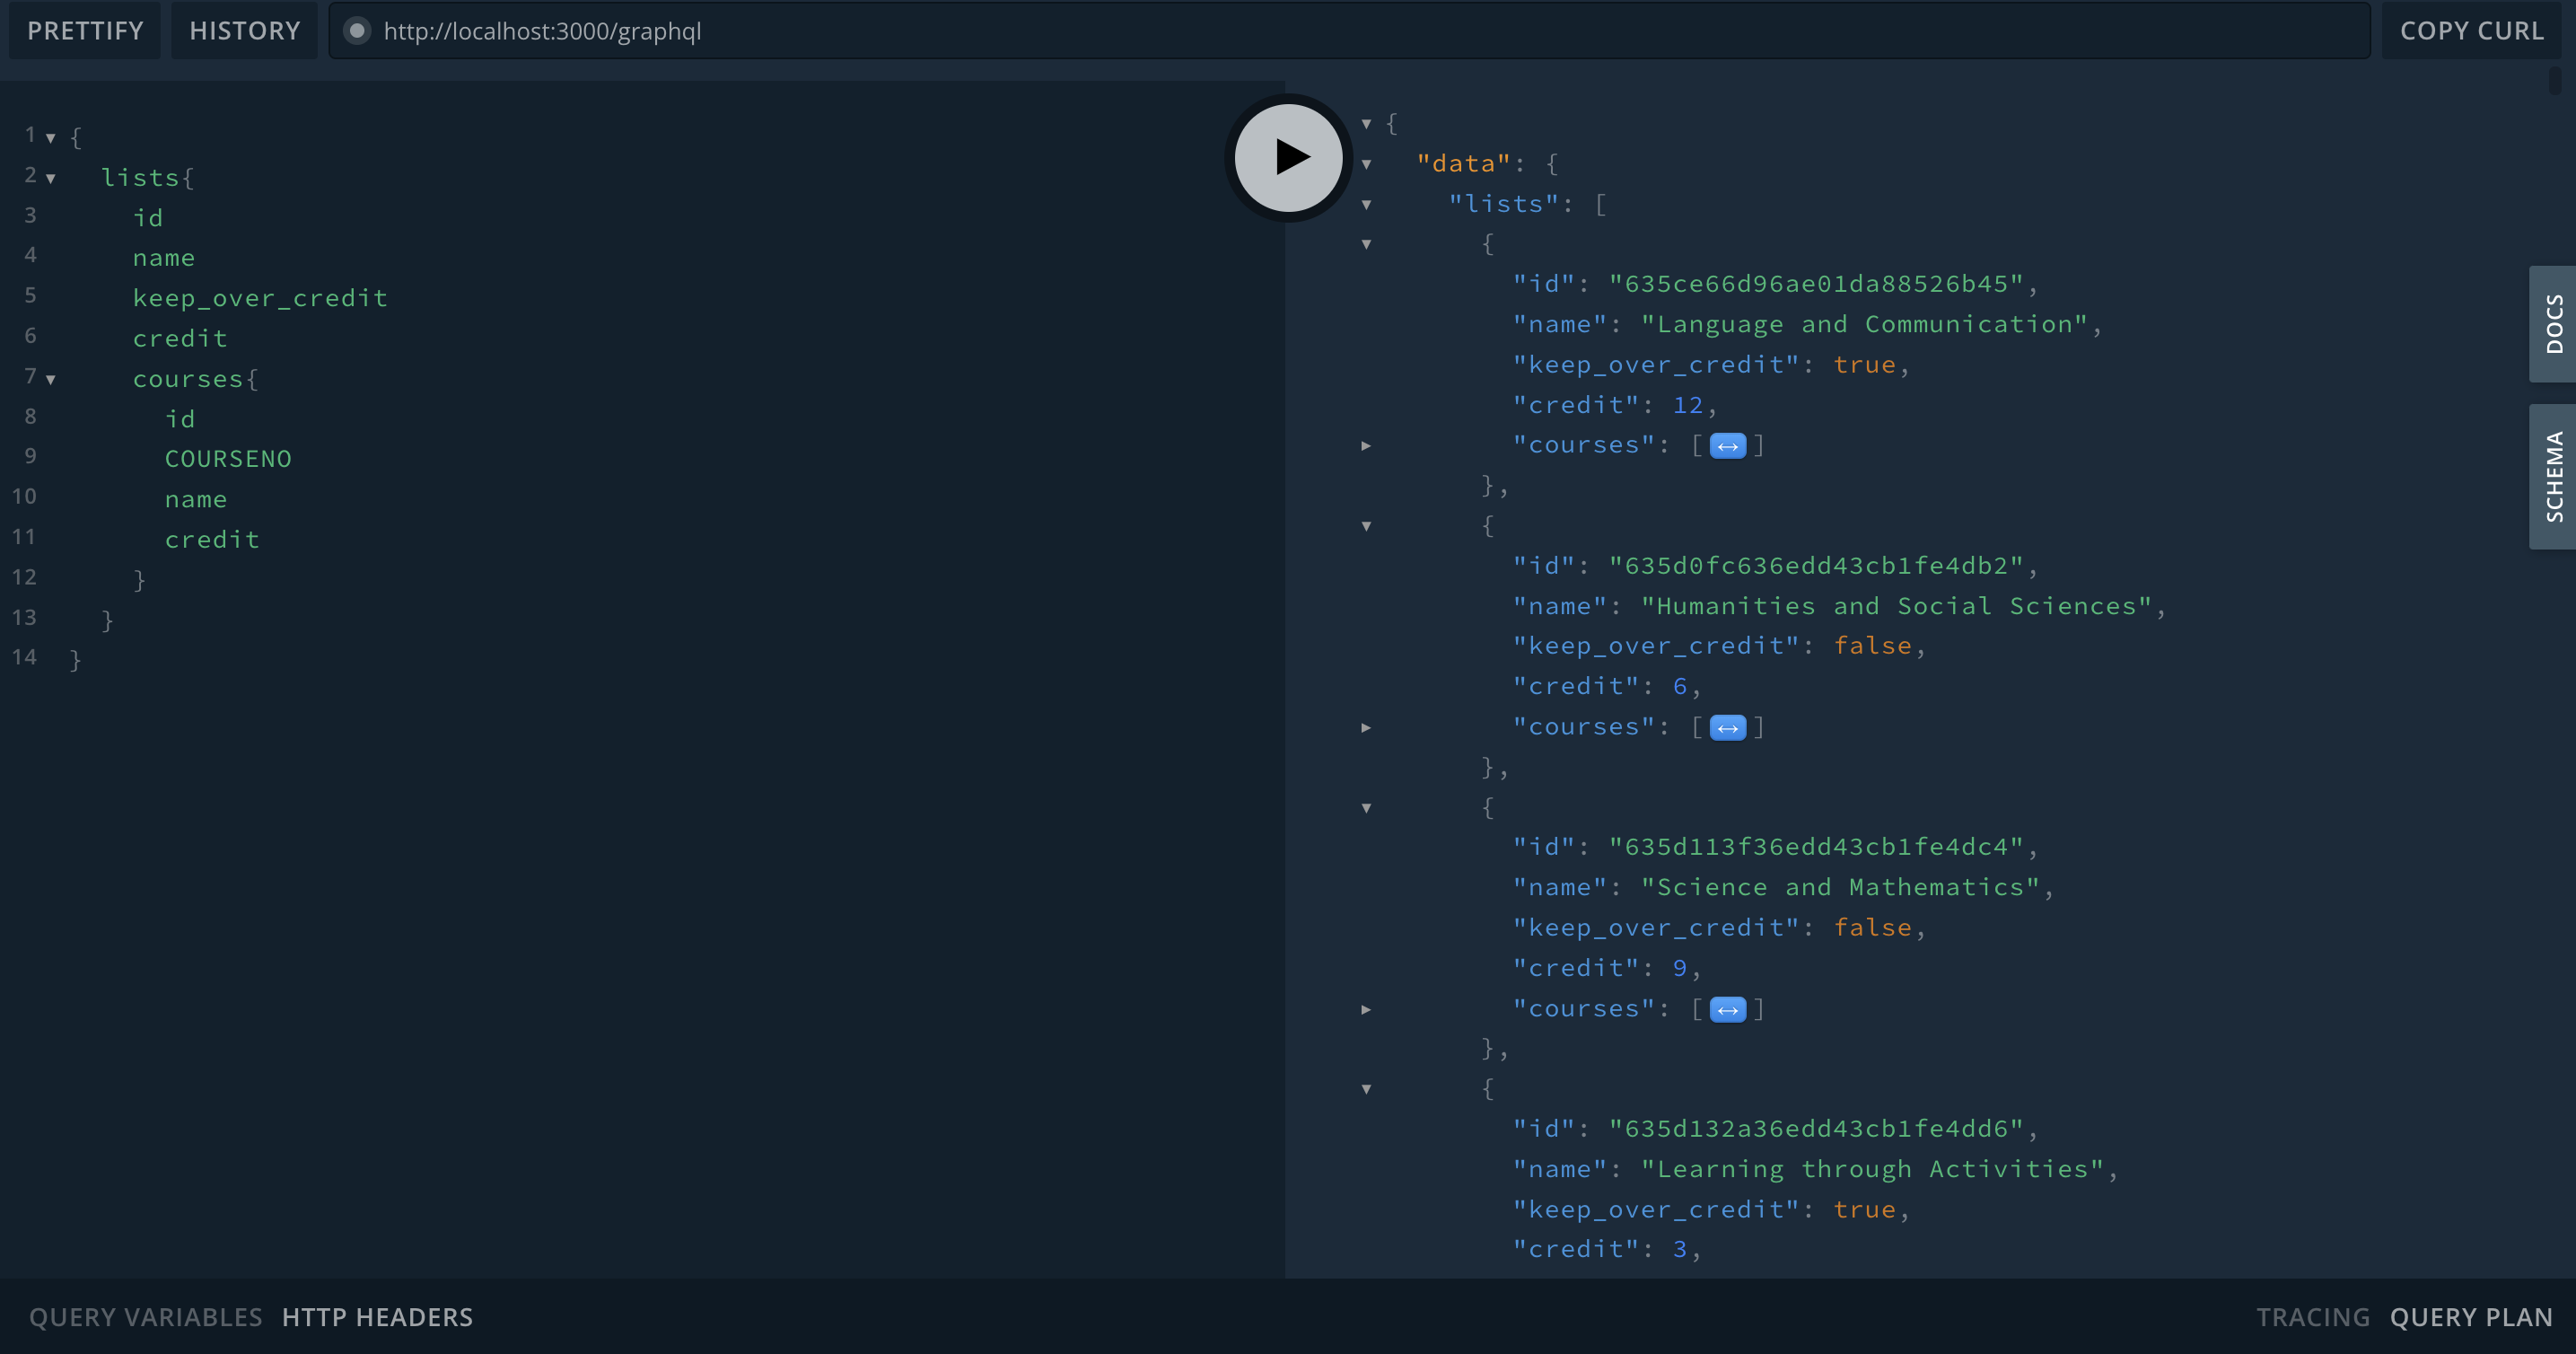
\includegraphics[width=0.8\textwidth]{gql.png}
      \caption{lists data}
      \label{fig:gql}
    \end{center}
  \end{figure}
    
\subsection{ผลตอบรับและความคิดเห็นของผู้ใช้งาน}
หลังจากการพัฒนาระบบแสดงความคืบหน้าในการสำเร็จการศึกษา 
ทางผู้พัฒนาได้ปล่อยเวอร์ชันทดลองใช้งานให้กับนักศึกษาและอาจารย์ในภาควิชาคอมพิวเตอร์และภาควิชาเทคโนโลยีสารสนเทศพร้อมทั้งแนบแบบสอบถาม
เพื่อเก็บความพึงพอใจต่อภาพรวม UX/UI และ flow ของระบบ โดยมีนักศึกษาที่เข้ามาทดลองใช้งานระบบรวม 11 คน 
(นับจำนวนจากข้อมูลใน database ที่มีการ login เข้ามาในระบบ) แต่กลับพบว่ามีนักศึกษาเพียง 6 คนเท่านั้นที่ทำการตอบแบบสอบถาม 
พบว่าผลตอบลัพธ์และความคิดเห็นของผู้ใช้งานที่มีต่อเว็บแอปพลิเคชันมีแนวโน้มที่ดี ซึ่งสามารถสรุปผลตอบลัพธ์ได้ดังรูปที่ 1 และ รูปที่ 2 
ซึ่งเป็นความพีงพอใจต่อการใช้งานและภาพรวมของเว็บแอปพลิเคชัน

\begin{figure}[H]
    \begin{center}
      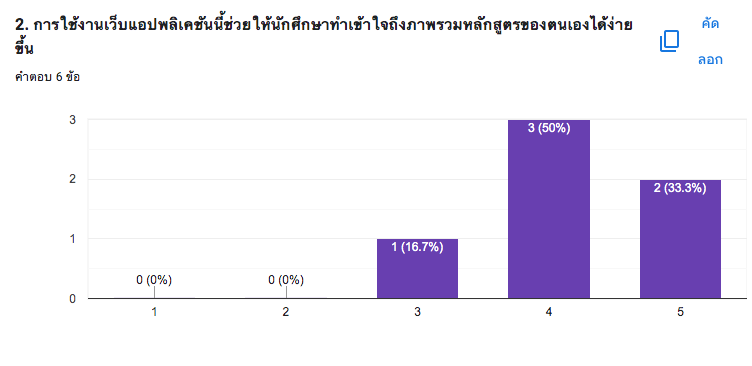
\includegraphics[width=0.8\textwidth]{toon1.png}
      \caption{ความพีงพอใจต่อการใช้งานและภาพรวมของเว็บแอปพลิเคชัน}
      \label{fig:toon1}
    \end{center}
\end{figure}

\begin{figure}[H]
    \begin{center}
      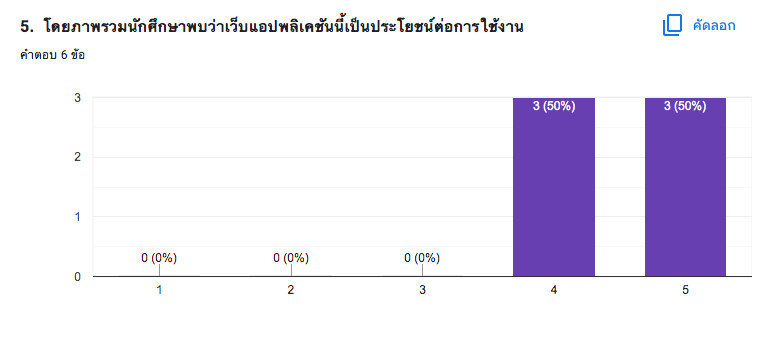
\includegraphics[width=0.8\textwidth]{toon2.png}
      \caption{ความพีงพอใจต่อภาพรวมของเว็บแอปพลิเคชัน}
      \label{fig:toon2}
    \end{center}
\end{figure}
    
\ifproject
\chapter{\ifenglish Conclusions and Discussions\else บทสรุปและข้อเสนอแนะ\fi}

\section{\ifenglish Conclusions\else สรุปผล\fi}

โครงงานระบบแสดงความคืบหน้าในการสำเร็จการศึกษา(Visualization system for graduation requirement fulfillment) 
จัดทำขึ้นเพื่อแก้ไขปัญหาความยุ่งยากในการตรวจสอบความคืบหน้าในการศึกษาของนักศึกษาจากวิธีเดิมที่จะต้องไล่ดูในหมวดวิชาต่างๆว่าลงเรียนวิชาในหมวดครบแล้วหรือยัง 
และช่วยให้นักศึกษาทำความเข้าใจหลักสูตรของตนเองได้ง่ายและเห็นภาพรวมของหลักสูตรเพื่อสามารถนำไปจัดการวางแผนการเรียนของตนเองได้ง่ายยิ่งขึ้น 
นอกจากนี้อาจารย์ที่ปรึกษาสามารถตรวจสอบความคืบหน้าในการศึกษาของนักศึกษาที่ตนเองดูแลอยู่ได้รวดเร็วและง่ายยิ่งขึ้น

\section{\ifenglish Challenges\else ปัญหาที่พบและแนวทางการแก้ไข\fi}

\subsection{Frontend}
\begin{itemize}
    \item  หน้าเว็บแอปพลิเคชันสำหรับอาจารย์ที่ปรึกษายังไม่ตอบโจทย์ต่อการใช้งานเท่าไรนัก 
    ควรเพิ่มเนื้อหาส่วนที่เป็นรายละเอียดของนักศึกษาเข้าไปด้วย เช่น tree-view 
    ของนักศึกษาคนแต่ละคนเพี่อให้ง่ายต่อการตรวจสอบความคืบหน้าของอาจารย์ที่ปรึกษา
    \item การ deploy มีข้อผิดพลาด คือหลังจากที่ผู้ใช้งาน login เข้าไปยังระบบหากเกิดข้อผิดพลาดในการดึงข้อมูลหน้าเว็บจะค้างที่หน้าสีขาว 
    ทำให้ผู้ใช้เกิดความสับสนและเสียเวลาในการรอหน้าเว็บแสดงข้อมูล ดังนั้นควรที่มีข้อความบอกถึงข้อผิดพลาดและสถานการณ์ดังกล่าวเพื่อแจ้งให้ผู้ใช้งานได้ทราบ
	
\end{itemize}

\subsection{Backend}
\begin{itemize}
    \item ในการประมวลผลเพื่อส่งข้อมูลไปยังหน้า student จําเป็นต้องใช้ หลาย query ทําให้ Frontend จําเป็นต้อง chain query หลายอันต่อเนื่องกัน ทําให้ระบบมีความช้าลง
	
\end{itemize}

\subsection{ปัญหาภาพรวม}
\begin{itemize}
    \item  หน้าเว็บแอปพลิเคชันสำหรับอาจารย์ที่ปรึกษายังไม่ตอบโจทย์ต่อการใช้งานเท่าไรนัก 
    ควรเพิ่มเนื้อหาส่วนที่เป็นรายละเอียดของนักศึกษาเข้าไปด้วย เช่น tree-view 
    ของนักศึกษาคนแต่ละคนเพี่อให้ง่ายต่อการตรวจสอบความคืบหน้าของอาจารย์ที่ปรึกษา
    \item หลังจากที่ผู้ใช้งาน login เข้าไปยังระบบหากเกิดข้อผิดพลาดในการดึงข้อมูลหน้าเว็บจะค้างที่หน้าสีขาว 
    ทำให้ผู้ใช้เกิดความสับสนและเสียเวลาในการรอหน้าเว็บแสดงข้อมูล ดังนั้นควรที่มีข้อความบอกถึงข้อผิดพลาดและสถานการณ์ดังกล่าวเพื่อแจ้งให้ผู้ใช้งานได้ทราบ
	
\end{itemize}


\section{\ifenglish%
Suggestions and further improvements
\else%
ข้อเสนอแนะและแนวทางการพัฒนาต่อ
\fi
}
\subsection{Frontend}
\begin{itemize}
    \item  หน้าเว็บแอปพลิเคชันสำหรับอาจารย์ที่ปรึกษายังไม่ตอบโจทย์ต่อการใช้งานเท่าไรนัก 
    ควรเพิ่มเนื้อหาส่วนที่เป็นรายละเอียดของนักศึกษาเข้าไปด้วย เช่น tree-view 
    ของนักศึกษาคนแต่ละคนเพี่อให้ง่ายต่อการตรวจสอบความคืบหน้าของอาจารย์ที่ปรึกษา
    \item หลังจากที่ผู้ใช้งาน login เข้าไปยังระบบหากเกิดข้อผิดพลาดในการดึงข้อมูลหน้าเว็บจะค้างที่หน้าสีขาว 
    ทำให้ผู้ใช้เกิดความสับสนและเสียเวลาในการรอหน้าเว็บแสดงข้อมูล ดังนั้นควรที่มีข้อความบอกถึงข้อผิดพลาดและสถานการณ์ดังกล่าวเพื่อแจ้งให้ผู้ใช้งานได้ทราบ
	
\end{itemize}

\subsection{Backend}
\begin{itemize}
    \item ระบบยังมีการประมวลผลที่ช้า เนื่องจากต้องเช็คข้อมูลใหม่ทุกครั้งที่มีการเรียก ควรเเก้ไขเป็นการเช็คเเค่ครั้งเดียวเเล้วเก็บ ข้อมูลทั้งหมดของนักศึกษาไว้
    \item ระบบยังไม่สามารถใช้กับ หลักสูตรระดับยากได้ เเต่การออกเเบบนั้นมีเเนวทางที่สามารถรองรับได้เเล้ว เเต่ยังขาดการทดลองจริง เพื่อหาข้อบกพร่องในการพัฒนาต่อ
	
\end{itemize}



\fi

\bibliography{myReport}

\ifproject
\normalspacing
\appendix
% \chapter{The first appendix}

Text for the first appendix goes here.

\section{Appendix section}

Text for a section in the first appendix goes here.

test ทดสอบฟอนต์ serif ภาษาไทย

\textsf{test ทดสอบฟอนต์ sans serif ภาษาไทย}

\verb+test ทดสอบฟอนต์ teletype ภาษาไทย+

\texttt{test ทดสอบฟอนต์ teletype ภาษาไทย}

\textbf{ตัวหนา serif ภาษาไทย \textsf{sans serif ภาษาไทย} \texttt{teletype ภาษาไทย}}

\textit{ตัวเอียง serif ภาษาไทย \textsf{sans serif ภาษาไทย} \texttt{teletype ภาษาไทย}}

\textbf{\textit{ตัวหนาเอียง serif ภาษาไทย \textsf{sans serif ภาษาไทย} \texttt{teletype ภาษาไทย}}}

\url{https://www.example.com/test_ทดสอบ_url}

\chapter{\ifenglish Manual\else คู่มือการใช้งานระบบ\fi}

Manual goes here.


%% Display glossary (optional) -- need glossary option.
\ifglossary\glossarypage\fi

%% Display index (optional) -- need idx option.
\ifindex\indexpage\fi

\begin{biosketch}
\begin{center}
  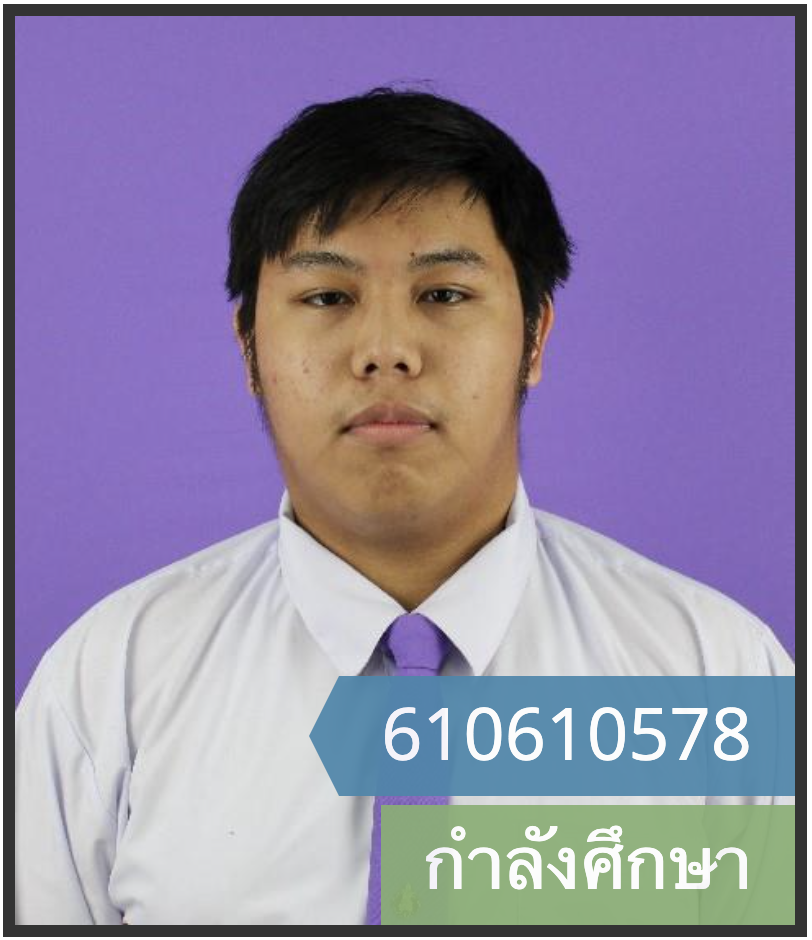
\includegraphics[width=1.5in]{hok.png}
\end{center}
นายชุติพนธ์ วิมลกาญจนา นักศึกษาชั้นปี ที่ 4 คณะวิศวกรรมศาสตร์ สาขาวิศวกรรมคอมพิวเตอร์ มหาวิทยาลัย
เชียงใหม่
\end{biosketch}

\begin{biosketch}
  \begin{center}
    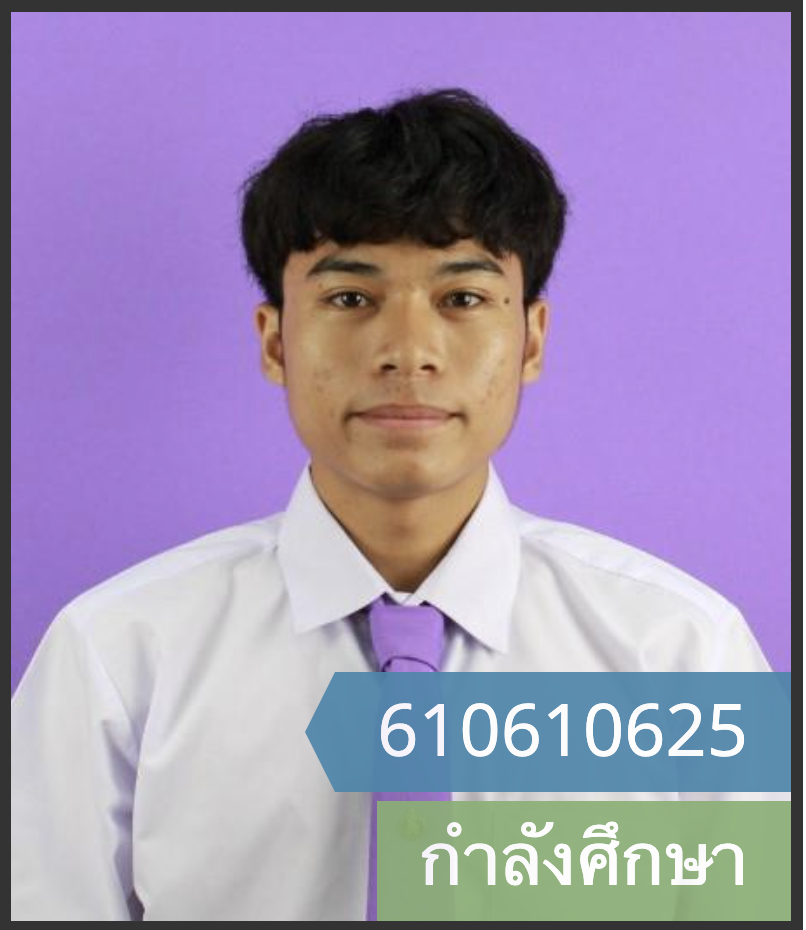
\includegraphics[width=1.5in]{toon.png}
  \end{center}
  นายอานนท์ รอดตัว นักศึกษาชั้นปี ที่ 4 คณะวิศวกรรมศาสตร์ สาขาวิศวกรรมคอมพิวเตอร์ มหาวิทยาลัย
  เชียงใหม่
  \end{biosketch}
  

\fi % \ifproject
\end{document}
